%%%%%%%%%%%%%%%%%%%%%%%%%%%%%%%%%%%%%%%%%%%%%%%%%%%%%%%%%%%%%%%%%%%%%%%%%%%%%%%%
\chapter{Finite Difference Methods}
\label{chap:fdm} % Always give a unique label
% use \chaptermark{}
% to alter or adjust the chapter heading in the running head

\abstract*{Each chapter should be preceded by an abstract (10--15 lines long) that summarizes the content. The abstract will appear \textit{online} at \url{www.SpringerLink.com} and be available with unrestricted access. This allows unregistered users to read the abstract as a teaser for the complete chapter. As a general rule the abstracts will not appear in the printed version of your book unless it is the style of your particular book or that of the series to which your book belongs.
Please use the 'starred' version of the new Springer \texttt{abstract} command for typesetting the text of the online abstracts (cf. source file of this chapter template \texttt{abstract}) and include them with the source files of your manuscript. Use the plain \texttt{abstract} command if the abstract is also to appear in the printed version of the book.}


\section{Taylor Series}
\label{sec:fdm_taylor}

% Reference Chapre and Canale
% Simple intro to Taylor Series
% Talk about truncation error

The finite difference method relies heavily on the mathematical concept of 
Taylor Series.\index{Taylor Series}  If we take a function, $f(x)$, the 
independent variable $x$ can be discretized into many points as shown in Figure \_.
If the value of the function is known at $x_{i}$, the value at $x_{i+1}$ can be
determined by a Taylor series expansion at $x_{i}$,
\begin{equation}
     f\left(x_{i+1}\right) = f\left(x_{i}\right) + f^{\prime}\left(x_{i}\right)h + 
     \frac{f^{\prime\prime}\left(x_{i}\right)}{2!}h^{2} + 
     \frac{f^{\left(3\right)}\left(x_{i}\right)}{3!}h^{3}+\cdot\cdot\cdot + 
     \frac{f^{\left(n\right)}\left(x_{i}\right)}{2!}h^{n} + \cdot\cdot\cdot
  \label{eq:fdm_taylor}
\end{equation}
In Eq. (\ref{eq:fdm_taylor}), $f^{\left(3\right)}$ represents the $n$-th derivative of 
the function and $h$ is the spacing between points, $h = x_{i+1} - x_{i}$.
\par
The expansion shown above is exact if the number of terms in the Taylor series
expansion is taken to infinity. Of course, this is not practical for computational
methods and therefore we truncate the series at a finite number of terms. The error
present caused by the truncation is known as truncation error.\index{truncation error}
Instead of representing the full Taylor expansion of a function, we will truncate
the expression after a few number of terms and repesent the truncation error with
$\mathcal{O}\left(h^{n}\right)$. In this representation of the truncation error,
$n$ represents the order of convergence.\index{order of convergence} Order of
convergence means that as the grid is refined by a factor of two for example, the
truncation error will reduce on the order of $2^{n}$. This does not imply that
one method is better than the order, just merely a concept of convergence rate
due to truncation effects. Linear convergence is when $n=1$, quadratic when $n=2$
and cubic when $n=3$. For example, if we expand a function to second order, we
would rewrite Eq. (\ref{eq:fdm_taylor}) this as
\begin{equation}
     f\left(x_{i+1}\right) = f\left(x_{i}\right) + f^{\prime}\left(x_{i}\right)h + 
     \frac{f^{\prime\prime}\left(x_{i}\right)}{2!}h^{2} + \mathcal{O}\left(h^{3}\right).
\end{equation}
As we approximate differentials, we can keep track of this truncation error to determine
order of convergence of our methods. This is one way to ensure that our discretization
method and implementation of solution algorithms are correct.

\section{Approximation of First Derivatives}
\label{sec:fdm_approx}

% Reference Chapre and Canale
% Forward, backward and central first order and second order differentials
% Simple example of Taylor expansion approximating with these approxs

There are many different approximations of differentials that can be constructed based
on Taylor series.  We will first consider the approximation of first order derivatives.
The first approximation is a \emph{first order forward difference} where we use information 
about a point just to the right, $x_{i+1}$, to infer the derivative at $x_{i}$.  If we 
perform a Taylor expansion about point $x_{i+1}$ to first order we get
\begin{equation}
     f\left(x_{i+1}\right) = f\left(x_{i}\right) + f^{\prime}\left(x_{i}\right)h + \mathcal{O}\left(h^{2}\right).
\end{equation}
This equation can be solved for the derivative of the function at $x_{i}$ 
\begin{equation}
     \boxed{f^{\prime}_{for}\left(x_{i}\right) = \frac{f\left(x_{i+1}\right) - f\left(x_{i}\right)}{h} - \mathcal{O}\left(h\right)},
  \label{eq:first_forward}
\end{equation}
where $f^{\prime}_{for}\left(x_{i}\right)$ represents the first order forward difference approximation to the derivative at
$x_{i}$.
\par
The opposite approximation is to consider a point to the left, $x_{i-1}$, to infer the
derivative at $x_{i}$, \emph{known as the first order backward difference}. Here, we take a Taylor expansion to the left,
\begin{equation}
     f\left(x_{i-1}\right) = f\left(x_{i}\right) - f^{\prime}\left(x_{i}\right)h + \mathcal{O}\left(h^{2}\right).
\end{equation}
Solving for the derivative we can arrive at
\begin{equation}
     \boxed{f^{\prime}_{bac}\left(x_{i}\right) = \frac{f\left(x_{i}\right) - f\left(x_{i-1}\right)}{h} + 
     \mathcal{O}\left(h\right).}
  \label{eq:first_backward}
\end{equation}
Comparing Eqs. (\ref{eq:first_forward}) and (\ref{eq:first_backward}) we see that the formulation looks the same in that it
is always the right point minus the left point in the numerator of the fraction. The only difference is the sign in the 
truncation error is reversed. Therefore, we can expect that one of these approximations will under-predict the true answer
and the other one will over-predict. Again both of these methods are first order methods.
\par 
The last simple approximation of a first derivative is a \emph{second-order central difference}. In this method we look 
at both left and right points. We can Taylor expand each of these to second order to get
\begin{eqnarray}
    f\left(x_{i+1}\right) = f\left(x_{i}\right) + f^{\prime}\left(x_{i}\right)h + \frac{f^{\prime\prime}\left(x_{i}\right)}{2!}h^{2} + \mathcal{O}\left(h^{3}\right) \\
    f\left(x_{i-1}\right) = f\left(x_{i}\right) - f^{\prime}\left(x_{i}\right)h + \frac{f^{\prime\prime}\left(x_{i}\right)}{2!}h^{2} - \mathcal{O}\left(h^{3}\right).
\end{eqnarray}
Subtracting the $x_{i-1}$ equation from the $x_{i+1}$, we are left with
\begin{equation}
    f\left(x_{i+1}\right) - f\left(x_{i-1}\right) = 2f^{\prime}\left(x_{i}\right)h  + \mathcal{O}\left(h^{3}\right).
\end{equation}
Solving for the derivative at $x_{i}$ we arrive at the second order central difference approximation
\begin{equation}
    \boxed{f^{\prime}_{cen}\left(x_{i}\right) = \frac{f\left(x_{i+1}\right) - f\left(x_{i-1}\right)}{2h} - \mathcal{O}\left(h^{2}\right).}
\end{equation}
From the resulting expression, this approximation method does not depend on the value of the function at $x_{i}$ and that
the scheme is second order convergent.
\par
\begin{figure}[t]
\sidecaption[t]
\scalebox{0.5}{\input{./figs/chap_fdm/fdm_approx_1.tikz}}
\caption{Convergence rate of forward, backward and central difference approximations. The slope of the error as a function of mesh spacing
is an estimate of the order of convergence of an approximation scheme.}
\label{fig:fdm_approx_1}
\end{figure}
\paragraph{Example - Order of Convergence First Derivative}
As a simple example, we can approximate the derivative of the function, $f\left(x\right) = x^{4}$, at $x=100$ with
each of the above approximations. We can choose an array of spacing values between $x_{i}$ and $x_{i+1}$ and $x_{i-1}$
and $x_{i}$. For each spacing value we compute the estimate of the derivative using the three approximations above.
To characterize the error of each we find the absolute difference between the approximation and the true value of the
derivative at $x=100$. To infer the order of convergence, we can graph the errors as a function of spacing on a 
log-log scale. These convergence plots are shown in Fig. \ref{fig:fdm_approx_1}.
\par 
There are two distinct convergence trends present in Fig. \ref{fig:fdm_approx_1}.  The curve with a slope of 1 on
the log-log scale represents forward and backward finite difference approximations. This shows that these methods
have linear convergence consistent with the truncation error. For the central difference approximation we predicted
that it would have quadratic convergence. We can see from the plot that the magnitude of the slope is 2 on the log-log scale.
MATLAB code to solve generate this plot is included below.
\lstinputlisting{./code/chap_fdm/fdm_approx_1.m}
% Discuss second order derivatives

\section{Approximation of Second Derivatives}

In nuclear reactor physics applications, we also need approximations for second derivatives.  The only difference in 
these approximations is that more points to the left or right of $x_{i}$ need to be included. For the \emph{first order
forward difference} approximation, we write two equations to second order. One equation representating a Taylor expansion
to $x_{i+1}$ and the other to $x_{i+2}$,
\begin{eqnarray}
    f\left(x_{i+1}\right) = f\left(x_{i}\right) + f^{\prime}\left(x_{i}\right)h + \frac{f^{\prime\prime}\left(x_{i}\right)}{2!}h^{2} + \mathcal{O}\left(h^{3}\right) 
  \label{eq:second_forward_1}
\\
    f\left(x_{i+2}\right) = f\left(x_{i}\right) + f^{\prime}\left(x_{i}\right)\left(2h\right) + \frac{f^{\prime\prime}\left(x_{i}\right)}{2!}\left(2h\right)^{2} + \mathcal{O}\left(h^{3}\right).
  \label{eq:second_forward_2}
\end{eqnarray}
Since we are approximating the second derivative, the first derivative needs to be canceled out. To cancel this term out, 
we multiply Eq. (\ref{eq:second_forward_1}) by a 2 and subtract it from Eq. (\ref{eq:second_forward_2}). The resulting 
expression is
\begin{equation}
    f\left(x_{i+2}\right) - 2f\left(x_{i+1}\right) = -f\left(x_{i}\right) + f^{\prime\prime}\left(x_{i}\right)h^{2} + \mathcal{O}\left(h^{3}\right).
\end{equation}
The approximation of the second derivative for a first-order forward difference is therefore
\begin{equation}
    \boxed{f^{\prime\prime}_{for}\left(x_{i}\right) = \frac{f\left(x_{i+2}\right) - 2f\left(x_{i+1}\right) + f\left(x_{i}\right)}{h^{2}} - \mathcal{O}\left(h\right).}
    \label{eq:second_forward}
\end{equation}
\par 
For the \emph{first-order backward finite difference} approximation of the second derivative we Taylor expand the function at
$x_{i-1}$ and $x_{i-2}$ 
\begin{eqnarray}
    f\left(x_{i-1}\right) = f\left(x_{i}\right) - f^{\prime}\left(x_{i}\right)h + \frac{f^{\prime\prime}\left(x_{i}\right)}{2!}h^{2} - \mathcal{O}\left(h^{3}\right) 
  \label{eq:second_backward_1}
\\
    f\left(x_{i-2}\right) = f\left(x_{i}\right) - f^{\prime}\left(x_{i}\right)\left(2h\right) + \frac{f^{\prime\prime}\left(x_{i}\right)}{2!}\left(2h\right)^{2} - \mathcal{O}\left(h^{3}\right).
  \label{eq:second_backward_2}
\end{eqnarray}
Similar to the forward finite difference case, we must eliminate the first derivative term by multiplying 
Eq. (\ref{eq:second_backward_1}) by 2 and subtract from Eq. (\ref{eq:second_backward_2}). This results in the following expression:
\begin{equation}
    f\left(x_{i-2}\right) - 2f\left(x_{i-1}\right) = -f\left(x_{i}\right) + f^{\prime\prime}\left(x_{i}\right)h^{2} - \mathcal{O}\left(h^{3}\right).
\end{equation}
The approximation of the second derivative for a first-order backward difference is therefore
\begin{equation}
    \boxed{f^{\prime\prime}_{bac}\left(x_{i}\right) = \frac{f\left(x_{i}\right) - 2f\left(x_{i-1}\right) + f\left(x_{i-2}\right)}{h^{2}} + \mathcal{O}\left(h\right).}
    \label{eq:second_backward}
\end{equation}
\par 
Lastly, the \emph{second-order central difference} approximation to the second derivative can be derived by performing 
a Taylor expansion at $x_{i-1}$ and $x_{i+1}$ to fourth-order,
\begin{eqnarray}
    f\left(x_{i+1}\right) = f\left(x_{i}\right) + f^{\prime}\left(x_{i}\right)h + \frac{f^{\prime\prime}\left(x_{i}\right)}{2!}h^{2} + \frac{f^{\prime\prime\prime}\left(x_{i}\right)}{3!}h^{3} + \mathcal{O}\left(h^{4}\right) \\
    f\left(x_{i-1}\right) = f\left(x_{i}\right) - f^{\prime}\left(x_{i}\right)h + \frac{f^{\prime\prime}\left(x_{i}\right)}{2!}h^{2} - \frac{f^{\prime\prime\prime}\left(x_{i}\right)}{3!}h^{3} + \mathcal{O}\left(h^{4}\right).
\end{eqnarray}
To eliminate the first derivate term, these two equations can be directly added together resulting in
\begin{equation}
    f\left(x_{i+1}\right) + f\left(x_{i-1}\right) = 2f\left(x_{i}\right) + f^{\prime\prime}\left(x_{i}\right)h^{2} + \mathcal{O}\left(h^{4}\right).
\end{equation}
The approximation of the second derivative for a second-order central difference is
\begin{equation}
    \boxed{f^{\prime\prime}_{cen}\left(x_{i}\right) = \frac{f\left(x_{i+1}\right) -2f\left(x_{i}\right) + f\left(x_{i-1}\right)}{h^{2}} - \mathcal{O}\left(h^{2}\right).}
     \label{eq:second_central}
\end{equation}
The second-order central difference will be the main approximation we use for second order derivatives. This is mainly due to the
fact that has quadratic convergence. The other reason is that for a given computational node in a reactor, we think of leakage
occuring to the left and to the right. This leakage term in represented with mathematically by a second derivative and by using
the central difference approximation, we can couple to both the right and left nodes.

\begin{figure}[t]
\sidecaption[t]
\scalebox{0.5}{% This file was created by matlab2tikz v0.1.4.
% Copyright (c) 2008--2011, Nico Schlömer <nico.schloemer@gmail.com>
% All rights reserved.
% 
% The latest updates can be retrieved from
%   http://www.mathworks.com/matlabcentral/fileexchange/22022-matlab2tikz
% where you can also make suggestions and rate matlab2tikz.
% 
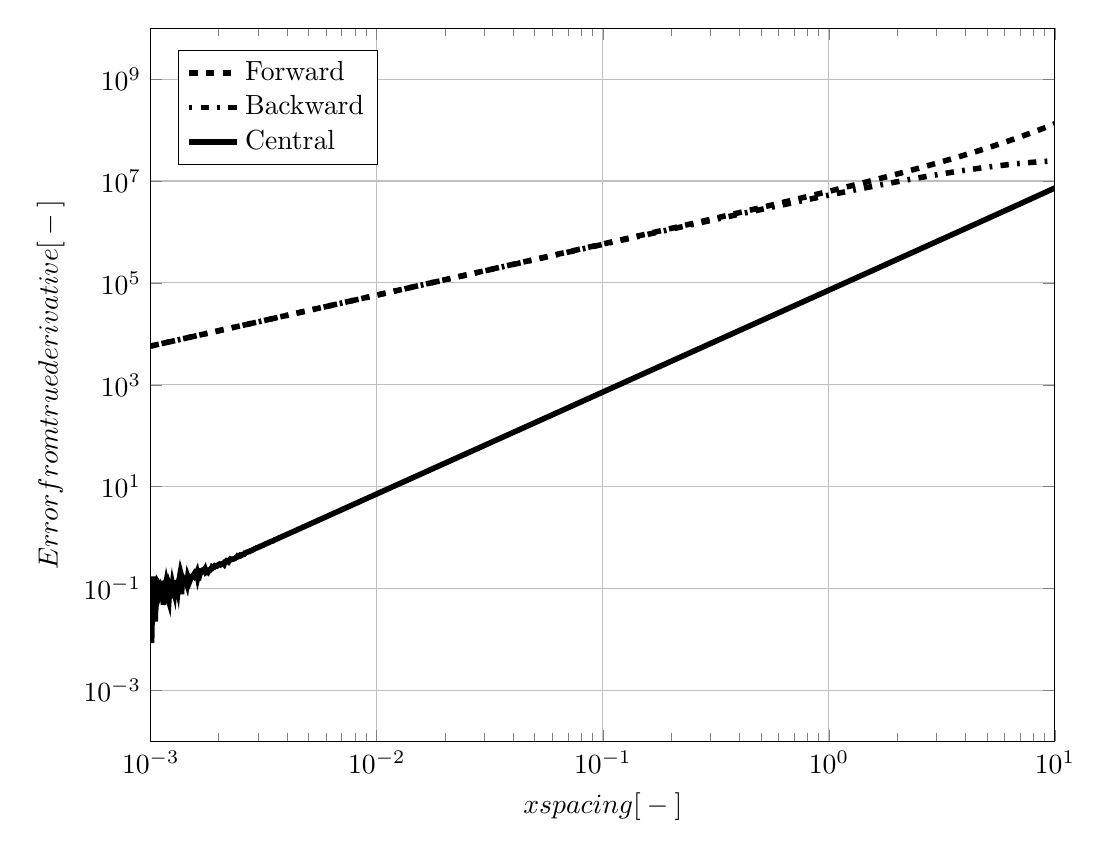
\begin{tikzpicture}

\begin{loglogaxis}[%
scale only axis,
width=4.52083in,
height=3.56562in,
xmin=0.001, xmax=10,
ymin=0.0001, ymax=1e+10,
xminorticks=true,
yminorticks=true,
xlabel={$\text{x spacing [}-\text{]}$},
ylabel={$\text{Error from true derivative [}-\text{]}$},
xmajorgrids,
ymajorgrids,
legend entries={Forward,Backward,Central},
legend style={at={(0.03,0.97)},anchor=north west,nodes=right}]
\addplot [
color=black,
dashed,
line width=2.0pt
]
coordinates{
 (0.001,5760.02)(0.00100926,5813.83)(0.00101861,5867.66)(0.00102804,5922.42)(0.00103757,5976.56)(0.00104718,6031.91)(0.00105688,6088.56)(0.00106666,6144.61)(0.00107654,6201.45)(0.00108652,6258.85)(0.00109658,6316.91)(0.00110674,6375.73)(0.00111699,6434.85)(0.00112733,6493.73)(0.00113777,6554.06)(0.00114831,6614.9)(0.00115895,6676)(0.00116968,6738.12)(0.00118052,6800.87)(0.00119145,6863.55)(0.00120249,6927.1)(0.00121362,6991.52)(0.00122486,7056.06)(0.00123621,7121.42)(0.00124766,7187.08)(0.00125922,7254.19)(0.00127088,7320.93)(0.00128265,7388.93)(0.00129453,7457.4)(0.00130652,7526.41)(0.00131862,7596.25)(0.00133083,7666.26)(0.00134316,7737.72)(0.0013556,7808.96)(0.00136816,7881.43)(0.00138083,7954.58)(0.00139362,8028.3)(0.00140653,8102.84)(0.00141955,8177.94)(0.0014327,8253.66)(0.00144597,8329.69)(0.00145937,8406.87)(0.00147288,8485.08)(0.00148652,8563.38)(0.00150029,8642.7)(0.00151419,8722.77)(0.00152821,8803.93)(0.00154237,8885.1)(0.00155665,8967.73)(0.00157107,9050.65)(0.00158562,9134.68)(0.00160031,9219.24)(0.00161513,9304.71)(0.00163009,9390.73)(0.00164519,9477.53)(0.00166043,9565.33)(0.00167581,9654.22)(0.00169133,9743.56)(0.00170699,9833.65)(0.00172281,9925.02)(0.00173876,10016.8)(0.00175487,10109.5)(0.00177112,10203.4)(0.00178753,10297.7)(0.00180408,10393.3)(0.00182079,10489.5)(0.00183766,10586.8)(0.00185468,10684.7)(0.00187186,10783.7)(0.00188919,10883.6)(0.00190669,10984.3)(0.00192435,11086.2)(0.00194217,11188.9)(0.00196016,11292.5)(0.00197832,11397.1)(0.00199664,11502.7)(0.00201514,11609.2)(0.0020338,11717)(0.00205264,11825.4)(0.00207165,11934.8)(0.00209084,12045.5)(0.0021102,12157.1)(0.00212975,12269.6)(0.00214947,12383.3)(0.00216938,12498.1)(0.00218948,12613.7)(0.00220976,12730.8)(0.00223022,12848.5)(0.00225088,12967.7)(0.00227173,13087.7)(0.00229277,13209.1)(0.00231401,13331.4)(0.00233544,13455)(0.00235707,13579.6)(0.0023789,13705.3)(0.00240093,13832.4)(0.00242317,13960.5)(0.00244562,14089.8)(0.00246827,14220.4)(0.00249113,14352)(0.0025142,14485.1)(0.00253749,14619.2)(0.00256099,14754.7)(0.00258471,14891.3)(0.00260865,15029.4)(0.00263282,15168.5)(0.0026572,15309)(0.00268181,15450.9)(0.00270665,15594.1)(0.00273172,15738.6)(0.00275702,15884.3)(0.00278256,16031.6)(0.00280833,16180)(0.00283434,16329.9)(0.0028606,16481.2)(0.00288709,16633.9)(0.00291383,16788)(0.00294082,16943.5)(0.00296806,17100.5)(0.00299555,17258.9)(0.00302329,17418.8)(0.0030513,17580.2)(0.00307956,17743.1)(0.00310808,17907.4)(0.00313687,18073.4)(0.00316592,18240.9)(0.00319525,18409.9)(0.00322484,18580.4)(0.00325471,18752.5)(0.00328486,18926.3)(0.00331528,19101.6)(0.00334599,19278.6)(0.00337698,19457.2)(0.00340826,19637.5)(0.00343983,19819.5)(0.00347169,20003.1)(0.00350384,20188.4)(0.0035363,20375.4)(0.00356905,20564.2)(0.00360211,20754.8)(0.00363547,20947.1)(0.00366914,21141.1)(0.00370313,21337)(0.00373743,21534.7)(0.00377204,21734.2)(0.00380698,21935.6)(0.00384224,22138.8)(0.00387783,22344)(0.00391375,22551)(0.00395,22760)(0.00398658,22970.8)(0.00402351,23183.7)(0.00406077,23398.5)(0.00409838,23615.3)(0.00413634,23834.1)(0.00417466,24054.9)(0.00421332,24277.8)(0.00425235,24502.7)(0.00429173,24729.7)(0.00433148,24958.9)(0.0043716,25190.2)(0.00441209,25423.6)(0.00445296,25659.1)(0.0044942,25896.9)(0.00453583,26136.9)(0.00457784,26379)(0.00462024,26623.5)(0.00466303,26870.2)(0.00470622,27119.1)(0.00474981,27370.4)(0.00479381,27624)(0.00483821,27880)(0.00488302,28138.3)(0.00492825,28399.1)(0.0049739,28662.2)(0.00501997,28927.8)(0.00506646,29195.9)(0.00511339,29466.4)(0.00516075,29739.5)(0.00520855,30015)(0.00525679,30293.2)(0.00530548,30573.9)(0.00535462,30857.2)(0.00540422,31143.1)(0.00545427,31431.7)(0.00550479,31723)(0.00555578,32017)(0.00560723,32313.7)(0.00565917,32613.1)(0.00571159,32915.3)(0.00576449,33220.4)(0.00581788,33528.2)(0.00587177,33838.9)(0.00592615,34152.5)(0.00598104,34469)(0.00603644,34788.4)(0.00609235,35110.8)(0.00614878,35436.2)(0.00620573,35764.6)(0.00626321,36096)(0.00632122,36430.5)(0.00637977,36768.1)(0.00643886,37108.9)(0.0064985,37452.8)(0.00655869,37799.9)(0.00661943,38150.2)(0.00668074,38503.8)(0.00674262,38860.6)(0.00680507,39220.7)(0.0068681,39584.2)(0.00693172,39951.1)(0.00699592,40321.3)(0.00706072,40695)(0.00712612,41072.2)(0.00719212,41452.8)(0.00725873,41837)(0.00732597,42224.8)(0.00739382,42616.1)(0.0074623,43011.1)(0.00753142,43409.8)(0.00760118,43812.1)(0.00767158,44218.2)(0.00774264,44628)(0.00781435,45041.6)(0.00788673,45459.1)(0.00795978,45880.4)(0.0080335,46305.7)(0.00810791,46734.9)(0.00818301,47168.1)(0.0082588,47605.3)(0.00833529,48046.5)(0.0084125,48491.9)(0.00849042,48941.3)(0.00856906,49395)(0.00864842,49852.8)(0.00872853,50314.9)(0.00880937,50781.3)(0.00889097,51252)(0.00897332,51727.1)(0.00905643,52206.6)(0.00914031,52690.5)(0.00922497,53179)(0.00931041,53671.9)(0.00939665,54169.4)(0.00948368,54671.6)(0.00957152,55178.4)(0.00966017,55689.9)(0.00974965,56206.1)(0.00983995,56727.2)(0.00993109,57253.1)(0.0100231,57783.8)(0.0101159,58319.5)(0.0102096,58860.1)(0.0103042,59405.8)(0.0103996,59956.5)(0.0104959,60512.4)(0.0105931,61073.4)(0.0106913,61639.6)(0.0107903,62211)(0.0108902,62787.8)(0.0109911,63369.9)(0.0110929,63957.4)(0.0111956,64550.4)(0.0112993,65148.8)(0.011404,65752.9)(0.0115096,66362.5)(0.0116162,66977.8)(0.0117238,67598.8)(0.0118324,68225.5)(0.011942,68858.1)(0.0120526,69496.6)(0.0121642,70140.9)(0.0122769,70791.3)(0.0123906,71447.7)(0.0125054,72110.2)(0.0126212,72778.8)(0.0127381,73453.7)(0.0128561,74134.8)(0.0129752,74822.2)(0.0130954,75516)(0.0132166,76216.3)(0.0133391,76923)(0.0134626,77636.3)(0.0135873,78356.3)(0.0137131,79082.9)(0.0138402,79816.3)(0.0139684,80556.4)(0.0140977,81303.5)(0.0142283,82057.5)(0.0143601,82818.5)(0.0144931,83586.5)(0.0146273,84361.7)(0.0147628,85144.1)(0.0148996,85933.7)(0.0150376,86730.7)(0.0151768,87535.1)(0.0153174,88346.9)(0.0154593,89166.3)(0.0156025,89993.3)(0.015747,90828)(0.0158928,91670.5)(0.01604,92520.7)(0.0161886,93378.9)(0.0163385,94245)(0.0164899,95119.2)(0.0166426,96001.5)(0.0167967,96892)(0.0169523,97790.7)(0.0171093,98697.8)(0.0172678,99613.4)(0.0174277,100537)(0.0175892,101470)(0.0177521,102411)(0.0179165,103361)(0.0180824,104320)(0.0182499,105288)(0.018419,106265)(0.0185896,107251)(0.0187617,108246)(0.0189355,109250)(0.0191109,110264)(0.0192879,111287)(0.0194666,112319)(0.0196469,113361)(0.0198288,114413)(0.0200125,115474)(0.0201979,116546)(0.0203849,117627)(0.0205737,118719)(0.0207643,119820)(0.0209566,120932)(0.0211507,122054)(0.0213466,123187)(0.0215443,124330)(0.0217439,125484)(0.0219453,126648)(0.0221486,127824)(0.0223537,129010)(0.0225607,130207)(0.0227697,131416)(0.0229806,132635)(0.0231935,133866)(0.0234083,135109)(0.0236251,136363)(0.0238439,137628)(0.0240648,138906)(0.0242876,140195)(0.0245126,141496)(0.0247396,142810)(0.0249688,144135)(0.0252,145473)(0.0254335,146824)(0.025669,148187)(0.0259068,149562)(0.0261467,150951)(0.0263889,152352)(0.0266333,153767)(0.02688,155194)(0.027129,156635)(0.0273803,158089)(0.0276339,159557)(0.0278898,161038)(0.0281481,162534)(0.0284088,164043)(0.028672,165566)(0.0289375,167103)(0.0292056,168655)(0.0294761,170221)(0.0297491,171802)(0.0300246,173397)(0.0303027,175008)(0.0305834,176633)(0.0308666,178273)(0.0311525,179929)(0.0314411,181600)(0.0317323,183287)(0.0320262,184989)(0.0323228,186708)(0.0326222,188442)(0.0329244,190192)(0.0332293,191959)(0.0335371,193742)(0.0338477,195542)(0.0341612,197359)(0.0344776,199192)(0.034797,201043)(0.0351193,202910)(0.0354446,204796)(0.0357729,206698)(0.0361042,208619)(0.0364386,210557)(0.0367761,212514)(0.0371167,214489)(0.0374605,216482)(0.0378075,218494)(0.0381576,220524)(0.0385111,222573)(0.0388678,224642)(0.0392278,226730)(0.0395911,228837)(0.0399578,230964)(0.0403279,233111)(0.0407014,235278)(0.0410784,237465)(0.0414589,239672)(0.0418429,241900)(0.0422304,244149)(0.0426216,246419)(0.0430164,248710)(0.0434148,251022)(0.0438169,253356)(0.0442227,255712)(0.0446323,258089)(0.0450457,260489)(0.045463,262911)(0.045884,265356)(0.046309,267824)(0.046738,270315)(0.0471708,272829)(0.0476078,275366)(0.0480487,277928)(0.0484937,280513)(0.0489429,283122)(0.0493962,285756)(0.0498537,288414)(0.0503155,291097)(0.0507815,293805)(0.0512519,296539)(0.0517266,299298)(0.0522057,302083)(0.0526892,304893)(0.0531772,307731)(0.0536698,310594)(0.0541669,313485)(0.0546686,316402)(0.0551749,319347)(0.055686,322319)(0.0562017,325319)(0.0567223,328347)(0.0572477,331404)(0.0577779,334489)(0.0583131,337603)(0.0588532,340746)(0.0593983,343918)(0.0599484,347120)(0.0605037,350352)(0.0610641,353615)(0.0616297,356908)(0.0622005,360231)(0.0627766,363586)(0.063358,366973)(0.0639449,370391)(0.0645372,373841)(0.0651349,377323)(0.0657382,380838)(0.0663471,384386)(0.0669616,387967)(0.0675818,391581)(0.0682078,395230)(0.0688395,398913)(0.0694771,402630)(0.0701206,406382)(0.0707701,410169)(0.0714256,413992)(0.0720872,417851)(0.0727548,421746)(0.0734287,425677)(0.0741088,429645)(0.0747952,433651)(0.075488,437694)(0.0761872,441775)(0.0768928,445894)(0.077605,450052)(0.0783238,454249)(0.0790493,458486)(0.0797814,462762)(0.0805204,467078)(0.0812662,471435)(0.0820189,475833)(0.0827786,480272)(0.0835453,484753)(0.0843191,489276)(0.0851001,493842)(0.0858883,498450)(0.0866838,503102)(0.0874867,507797)(0.088297,512537)(0.0891148,517321)(0.0899402,522151)(0.0907733,527025)(0.091614,531946)(0.0924626,536913)(0.093319,541926)(0.0941833,546987)(0.0950557,552095)(0.0959361,557252)(0.0968247,562457)(0.0977215,567711)(0.0986266,573015)(0.0995401,578368)(0.100462,583772)(0.101393,589227)(0.102332,594734)(0.103279,600292)(0.104236,605903)(0.105202,611566)(0.106176,617283)(0.107159,623054)(0.108152,628880)(0.109154,634760)(0.110165,640696)(0.111185,646688)(0.112215,652737)(0.113254,658843)(0.114303,665006)(0.115362,671227)(0.11643,677508)(0.117509,683848)(0.118597,690247)(0.119696,696707)(0.120804,703229)(0.121923,709811)(0.123052,716457)(0.124192,723165)(0.125342,729936)(0.126503,736772)(0.127675,743672)(0.128858,750638)(0.130051,757670)(0.131256,764768)(0.132471,771933)(0.133698,779167)(0.134937,786469)(0.136187,793840)(0.137448,801281)(0.138721,808793)(0.140006,816376)(0.141303,824031)(0.142611,831758)(0.143932,839559)(0.145265,847434)(0.146611,855384)(0.147969,863409)(0.149339,871511)(0.150723,879689)(0.152119,887945)(0.153528,896280)(0.15495,904694)(0.156385,913188)(0.157833,921763)(0.159295,930420)(0.16077,939159)(0.16226,947981)(0.163762,956887)(0.165279,965878)(0.16681,974955)(0.168355,984118)(0.169914,993368)(0.171488,1.00271e+06)(0.173077,1.01213e+06)(0.17468,1.02165e+06)(0.176298,1.03126e+06)(0.17793,1.04096e+06)(0.179578,1.05075e+06)(0.181242,1.06064e+06)(0.18292,1.07062e+06)(0.184615,1.0807e+06)(0.186325,1.09087e+06)(0.18805,1.10114e+06)(0.189792,1.11151e+06)(0.19155,1.12198e+06)(0.193324,1.13255e+06)(0.195115,1.14321e+06)(0.196922,1.15399e+06)(0.198746,1.16486e+06)(0.200587,1.17584e+06)(0.202445,1.18692e+06)(0.20432,1.19811e+06)(0.206212,1.20941e+06)(0.208122,1.22081e+06)(0.21005,1.23233e+06)(0.211995,1.24396e+06)(0.213959,1.25569e+06)(0.215941,1.26754e+06)(0.217941,1.27951e+06)(0.219959,1.29159e+06)(0.221997,1.30378e+06)(0.224053,1.31609e+06)(0.226128,1.32852e+06)(0.228222,1.34108e+06)(0.230336,1.35375e+06)(0.23247,1.36654e+06)(0.234623,1.37946e+06)(0.236796,1.3925e+06)(0.238989,1.40567e+06)(0.241203,1.41896e+06)(0.243437,1.43238e+06)(0.245692,1.44594e+06)(0.247967,1.45962e+06)(0.250264,1.47343e+06)(0.252582,1.48738e+06)(0.254921,1.50147e+06)(0.257283,1.51569e+06)(0.259666,1.53004e+06)(0.262071,1.54454e+06)(0.264498,1.55918e+06)(0.266948,1.57395e+06)(0.26942,1.58888e+06)(0.271916,1.60394e+06)(0.274434,1.61916e+06)(0.276976,1.63452e+06)(0.279542,1.65002e+06)(0.282131,1.66568e+06)(0.284744,1.6815e+06)(0.287381,1.69746e+06)(0.290043,1.71358e+06)(0.292729,1.72986e+06)(0.295441,1.7463e+06)(0.298177,1.76289e+06)(0.300939,1.77965e+06)(0.303726,1.79657e+06)(0.30654,1.81366e+06)(0.309379,1.83091e+06)(0.312244,1.84833e+06)(0.315136,1.86593e+06)(0.318055,1.88369e+06)(0.321001,1.90163e+06)(0.323974,1.91974e+06)(0.326975,1.93803e+06)(0.330003,1.9565e+06)(0.33306,1.97514e+06)(0.336145,1.99398e+06)(0.339258,2.01299e+06)(0.342401,2.0322e+06)(0.345572,2.05159e+06)(0.348773,2.07117e+06)(0.352003,2.09094e+06)(0.355263,2.11091e+06)(0.358554,2.13108e+06)(0.361875,2.15144e+06)(0.365227,2.172e+06)(0.36861,2.19277e+06)(0.372024,2.21374e+06)(0.375469,2.23492e+06)(0.378947,2.2563e+06)(0.382457,2.2779e+06)(0.385999,2.29971e+06)(0.389575,2.32174e+06)(0.393183,2.34398e+06)(0.396825,2.36644e+06)(0.4005,2.38913e+06)(0.40421,2.41204e+06)(0.407953,2.43518e+06)(0.411732,2.45854e+06)(0.415546,2.48214e+06)(0.419394,2.50598e+06)(0.423279,2.53005e+06)(0.427199,2.55435e+06)(0.431156,2.57891e+06)(0.43515,2.6037e+06)(0.43918,2.62874e+06)(0.443248,2.65403e+06)(0.447353,2.67958e+06)(0.451497,2.70538e+06)(0.455679,2.73143e+06)(0.459899,2.75775e+06)(0.464159,2.78433e+06)(0.468458,2.81117e+06)(0.472797,2.83829e+06)(0.477176,2.86567e+06)(0.481596,2.89333e+06)(0.486056,2.92127e+06)(0.490558,2.94949e+06)(0.495102,2.97799e+06)(0.499688,3.00677e+06)(0.504316,3.03585e+06)(0.508987,3.06522e+06)(0.513701,3.09489e+06)(0.518459,3.12485e+06)(0.523261,3.15512e+06)(0.528108,3.18569e+06)(0.532999,3.21657e+06)(0.537936,3.24776e+06)(0.542919,3.27927e+06)(0.547947,3.3111e+06)(0.553022,3.34325e+06)(0.558145,3.37573e+06)(0.563314,3.40853e+06)(0.568532,3.44167e+06)(0.573798,3.47515e+06)(0.579112,3.50896e+06)(0.584476,3.54313e+06)(0.58989,3.57763e+06)(0.595353,3.61249e+06)(0.600868,3.64771e+06)(0.606433,3.68329e+06)(0.61205,3.71923e+06)(0.617719,3.75553e+06)(0.62344,3.79221e+06)(0.629215,3.82927e+06)(0.635043,3.8667e+06)(0.640924,3.90452e+06)(0.646861,3.94273e+06)(0.652852,3.98133e+06)(0.658899,4.02033e+06)(0.665002,4.05973e+06)(0.671161,4.09954e+06)(0.677378,4.13976e+06)(0.683652,4.18039e+06)(0.689984,4.22145e+06)(0.696374,4.26292e+06)(0.702824,4.30483e+06)(0.709334,4.34717e+06)(0.715904,4.38996e+06)(0.722535,4.43318e+06)(0.729227,4.47686e+06)(0.735981,4.52099e+06)(0.742798,4.56558e+06)(0.749678,4.61064e+06)(0.756622,4.65617e+06)(0.76363,4.70217e+06)(0.770703,4.74865e+06)(0.777841,4.79562e+06)(0.785046,4.84309e+06)(0.792317,4.89105e+06)(0.799655,4.93951e+06)(0.807062,4.98849e+06)(0.814537,5.03798e+06)(0.822082,5.08799e+06)(0.829696,5.13853e+06)(0.837381,5.18961e+06)(0.845137,5.24122e+06)(0.852964,5.29338e+06)(0.860865,5.34609e+06)(0.868838,5.39937e+06)(0.876886,5.45321e+06)(0.885007,5.50762e+06)(0.893205,5.56261e+06)(0.901478,5.61818e+06)(0.909827,5.67435e+06)(0.918254,5.73112e+06)(0.926759,5.7885e+06)(0.935343,5.84649e+06)(0.944006,5.90511e+06)(0.95275,5.96435e+06)(0.961575,6.02423e+06)(0.970481,6.08475e+06)(0.97947,6.14593e+06)(0.988542,6.20776e+06)(0.997698,6.27026e+06)(1.00694,6.33344e+06)(1.01627,6.39731e+06)(1.02568,6.46186e+06)(1.03518,6.52712e+06)(1.04477,6.59309e+06)(1.05444,6.65977e+06)(1.06421,6.72718e+06)(1.07407,6.79533e+06)(1.08401,6.86422e+06)(1.09405,6.93387e+06)(1.10419,7.00427e+06)(1.11442,7.07546e+06)(1.12474,7.14742e+06)(1.13515,7.22017e+06)(1.14567,7.29373e+06)(1.15628,7.3681e+06)(1.16699,7.44329e+06)(1.1778,7.51931e+06)(1.18871,7.59617e+06)(1.19972,7.67389e+06)(1.21083,7.75247e+06)(1.22204,7.83193e+06)(1.23336,7.91227e+06)(1.24479,7.9935e+06)(1.25632,8.07565e+06)(1.26795,8.15871e+06)(1.2797,8.24271e+06)(1.29155,8.32765e+06)(1.30351,8.41355e+06)(1.31559,8.50041e+06)(1.32777,8.58825e+06)(1.34007,8.67708e+06)(1.35248,8.76692e+06)(1.36501,8.85778e+06)(1.37765,8.94967e+06)(1.39041,9.04261e+06)(1.40329,9.1366e+06)(1.41629,9.23166e+06)(1.4294,9.32781e+06)(1.44264,9.42506e+06)(1.45601,9.52343e+06)(1.46949,9.62293e+06)(1.4831,9.72356e+06)(1.49684,9.82536e+06)(1.5107,9.92834e+06)(1.5247,1.00325e+07)(1.53882,1.01379e+07)(1.55307,1.02445e+07)(1.56746,1.03523e+07)(1.58197,1.04614e+07)(1.59663,1.05717e+07)(1.61141,1.06834e+07)(1.62634,1.07963e+07)(1.6414,1.09106e+07)(1.65661,1.10262e+07)(1.67195,1.11432e+07)(1.68744,1.12616e+07)(1.70307,1.13813e+07)(1.71884,1.15025e+07)(1.73476,1.16251e+07)(1.75083,1.17492e+07)(1.76704,1.18747e+07)(1.78341,1.20018e+07)(1.79993,1.21303e+07)(1.8166,1.22604e+07)(1.83343,1.23921e+07)(1.85041,1.25253e+07)(1.86755,1.26601e+07)(1.88484,1.27966e+07)(1.9023,1.29347e+07)(1.91992,1.30745e+07)(1.9377,1.3216e+07)(1.95565,1.33592e+07)(1.97376,1.35041e+07)(1.99205,1.36508e+07)(2.0105,1.37993e+07)(2.02912,1.39497e+07)(2.04791,1.41018e+07)(2.06688,1.42559e+07)(2.08602,1.44118e+07)(2.10535,1.45697e+07)(2.12485,1.47295e+07)(2.14453,1.48913e+07)(2.16439,1.50551e+07)(2.18444,1.5221e+07)(2.20467,1.53889e+07)(2.22509,1.5559e+07)(2.2457,1.57311e+07)(2.2665,1.59054e+07)(2.28749,1.6082e+07)(2.30868,1.62607e+07)(2.33006,1.64417e+07)(2.35164,1.6625e+07)(2.37342,1.68107e+07)(2.39541,1.69987e+07)(2.41759,1.71891e+07)(2.43999,1.73819e+07)(2.46259,1.75772e+07)(2.48539,1.77751e+07)(2.50842,1.79754e+07)(2.53165,1.81784e+07)(2.5551,1.8384e+07)(2.57876,1.85922e+07)(2.60265,1.88032e+07)(2.62675,1.90169e+07)(2.65108,1.92334e+07)(2.67564,1.94527e+07)(2.70042,1.96749e+07)(2.72543,1.99001e+07)(2.75068,2.01282e+07)(2.77615,2.03593e+07)(2.80187,2.05935e+07)(2.82782,2.08308e+07)(2.85401,2.10712e+07)(2.88044,2.13149e+07)(2.90712,2.15619e+07)(2.93405,2.18121e+07)(2.96123,2.20657e+07)(2.98865,2.23227e+07)(3.01633,2.25833e+07)(3.04427,2.28473e+07)(3.07247,2.31149e+07)(3.10093,2.33862e+07)(3.12965,2.36612e+07)(3.15864,2.39399e+07)(3.18789,2.42225e+07)(3.21742,2.4509e+07)(3.24722,2.47994e+07)(3.27729,2.50938e+07)(3.30765,2.53924e+07)(3.33829,2.5695e+07)(3.36921,2.60019e+07)(3.40041,2.63131e+07)(3.43191,2.66287e+07)(3.46369,2.69487e+07)(3.49578,2.72732e+07)(3.52815,2.76022e+07)(3.56083,2.7936e+07)(3.59381,2.82745e+07)(3.6271,2.86178e+07)(3.6607,2.8966e+07)(3.6946,2.93193e+07)(3.72882,2.96776e+07)(3.76336,3.0041e+07)(3.79822,3.04097e+07)(3.8334,3.07838e+07)(3.8689,3.11633e+07)(3.90474,3.15483e+07)(3.9409,3.19389e+07)(3.9774,3.23353e+07)(4.01424,3.27375e+07)(4.05142,3.31456e+07)(4.08895,3.35597e+07)(4.12682,3.398e+07)(4.16504,3.44066e+07)(4.20362,3.48395e+07)(4.24256,3.52788e+07)(4.28185,3.57248e+07)(4.32151,3.61774e+07)(4.36154,3.66369e+07)(4.40194,3.71034e+07)(4.44271,3.75769e+07)(4.48386,3.80576e+07)(4.52539,3.85456e+07)(4.5673,3.90411e+07)(4.6096,3.95443e+07)(4.6523,4.00551e+07)(4.69539,4.05739e+07)(4.73888,4.11007e+07)(4.78277,4.16356e+07)(4.82707,4.2179e+07)(4.87178,4.27307e+07)(4.9169,4.32912e+07)(4.96244,4.38604e+07)(5.00841,4.44387e+07)(5.0548,4.5026e+07)(5.10162,4.56227e+07)(5.14887,4.62289e+07)(5.19656,4.68448e+07)(5.24469,4.74705e+07)(5.29327,4.81063e+07)(5.34229,4.87523e+07)(5.39177,4.94087e+07)(5.44171,5.00758e+07)(5.49212,5.07538e+07)(5.54299,5.14428e+07)(5.59433,5.2143e+07)(5.64614,5.28548e+07)(5.69844,5.35782e+07)(5.75122,5.43137e+07)(5.80449,5.50613e+07)(5.85825,5.58213e+07)(5.91251,5.6594e+07)(5.96727,5.73796e+07)(6.02254,5.81783e+07)(6.07832,5.89906e+07)(6.13462,5.98165e+07)(6.19144,6.06564e+07)(6.24879,6.15106e+07)(6.30667,6.23793e+07)(6.36508,6.32629e+07)(6.42403,6.41616e+07)(6.48353,6.50758e+07)(6.54359,6.60058e+07)(6.60419,6.69519e+07)(6.66536,6.79144e+07)(6.7271,6.88937e+07)(6.78941,6.989e+07)(6.85229,7.09039e+07)(6.91576,7.19356e+07)(6.97981,7.29855e+07)(7.04446,7.4054e+07)(7.10971,7.51414e+07)(7.17556,7.62482e+07)(7.24202,7.73749e+07)(7.3091,7.85217e+07)(7.3768,7.96891e+07)(7.44512,8.08776e+07)(7.51408,8.20877e+07)(7.58368,8.33197e+07)(7.65392,8.45741e+07)(7.72481,8.58515e+07)(7.79636,8.71523e+07)(7.86857,8.84771e+07)(7.94145,8.98263e+07)(8.01501,9.12005e+07)(8.08924,9.26002e+07)(8.16417,9.4026e+07)(8.23979,9.54785e+07)(8.3161,9.69582e+07)(8.39313,9.84658e+07)(8.47087,1.00002e+08)(8.54933,1.01567e+08)(8.62851,1.03162e+08)(8.70843,1.04787e+08)(8.78909,1.06443e+08)(8.8705,1.08131e+08)(8.95266,1.09852e+08)(9.03558,1.11606e+08)(9.11927,1.13394e+08)(9.20373,1.15216e+08)(9.28898,1.17074e+08)(9.37502,1.18969e+08)(9.46185,1.20901e+08)(9.54949,1.2287e+08)(9.63793,1.24879e+08)(9.7272,1.26927e+08)(9.8173,1.29016e+08)(9.90823,1.31147e+08)(10,1.3332e+08) 
};

\addplot [
color=black,
dash pattern=on 1pt off 3pt on 3pt off 3pt,
line width=2.0pt
]
coordinates{
 (0.001,5759.05)(0.00100926,5812.76)(0.00101861,5866.66)(0.00102804,5921.46)(0.00103757,5975.49)(0.00104718,6030.73)(0.00105688,6087.48)(0.00106666,6143.46)(0.00107654,6200.42)(0.00108652,6257.7)(0.00109658,6315.75)(0.00110674,6374.56)(0.00111699,6433.57)(0.00112733,6492.46)(0.00113777,6552.67)(0.00114831,6613.67)(0.00115895,6674.59)(0.00116968,6736.77)(0.00118052,6799.46)(0.00119145,6862.04)(0.00120249,6925.51)(0.00121362,6990.01)(0.00122486,7054.52)(0.00123621,7119.84)(0.00124766,7185.54)(0.00125922,7252.53)(0.00127088,7319.21)(0.00128265,7387.33)(0.00129453,7455.64)(0.00130652,7524.66)(0.00131862,7594.46)(0.00133083,7664.48)(0.00134316,7735.95)(0.0013556,7807.11)(0.00136816,7879.43)(0.00138083,7952.71)(0.00139362,8026.31)(0.00140653,8100.83)(0.00141955,8175.88)(0.0014327,8251.58)(0.00144597,8327.53)(0.00145937,8404.74)(0.00147288,8482.93)(0.00148652,8561.11)(0.00150029,8640.41)(0.00151419,8720.43)(0.00152821,8801.59)(0.00154237,8882.76)(0.00155665,8965.35)(0.00157107,9048.17)(0.00158562,9132.15)(0.00160031,9216.73)(0.00161513,9302.04)(0.00163009,9388.05)(0.00164519,9474.78)(0.00166043,9562.58)(0.00167581,9651.41)(0.00169133,9740.71)(0.00170699,9830.74)(0.00172281,9922.03)(0.00173876,10013.8)(0.00175487,10106.4)(0.00177112,10200.2)(0.00178753,10294.4)(0.00180408,10390)(0.00182079,10486.1)(0.00183766,10583.3)(0.00185468,10681.2)(0.00187186,10780.2)(0.00188919,10880)(0.00190669,10980.6)(0.00192435,11082.5)(0.00194217,11185.1)(0.00196016,11288.7)(0.00197832,11393.2)(0.00199664,11498.7)(0.00201514,11605.1)(0.0020338,11712.8)(0.00205264,11821.1)(0.00207165,11930.5)(0.00209084,12041.1)(0.0021102,12152.5)(0.00212975,12265)(0.00214947,12378.7)(0.00216938,12493.3)(0.00218948,12608.9)(0.00220976,12725.9)(0.00223022,12843.5)(0.00225088,12962.6)(0.00227173,13082.5)(0.00229277,13203.8)(0.00231401,13325.9)(0.00233544,13449.5)(0.00235707,13574)(0.0023789,13699.6)(0.00240093,13826.5)(0.00242317,13954.6)(0.00244562,14083.8)(0.00246827,14214.3)(0.00249113,14345.8)(0.0025142,14478.7)(0.00253749,14612.7)(0.00256099,14748.1)(0.00258471,14884.6)(0.00260865,15022.5)(0.00263282,15161.5)(0.0026572,15301.9)(0.00268181,15443.7)(0.00270665,15586.7)(0.00273172,15731.1)(0.00275702,15876.6)(0.00278256,16023.8)(0.00280833,16172)(0.00283434,16321.8)(0.0028606,16473)(0.00288709,16625.5)(0.00291383,16779.4)(0.00294082,16934.8)(0.00296806,17091.7)(0.00299555,17249.9)(0.00302329,17409.6)(0.0030513,17570.9)(0.00307956,17733.5)(0.00310808,17897.7)(0.00313687,18063.5)(0.00316592,18230.8)(0.00319525,18399.6)(0.00322484,18569.9)(0.00325471,18741.9)(0.00328486,18915.4)(0.00331528,19090.5)(0.00334599,19267.3)(0.00337698,19445.7)(0.00340826,19625.8)(0.00343983,19807.5)(0.00347169,19990.9)(0.00350384,20176)(0.0035363,20362.8)(0.00356905,20551.4)(0.00360211,20741.7)(0.00363547,20933.8)(0.00366914,21127.6)(0.00370313,21323.2)(0.00373743,21520.6)(0.00377204,21719.9)(0.00380698,21921)(0.00384224,22124)(0.00387783,22328.8)(0.00391375,22535.5)(0.00395,22744.2)(0.00398658,22954.8)(0.00402351,23167.3)(0.00406077,23381.9)(0.00409838,23598.3)(0.00413634,23816.8)(0.00417466,24037.3)(0.00421332,24259.9)(0.00425235,24484.5)(0.00429173,24711.2)(0.00433148,24940)(0.0043716,25170.9)(0.00441209,25404)(0.00445296,25639.1)(0.0044942,25876.5)(0.00453583,26116.1)(0.00457784,26357.9)(0.00462024,26602)(0.00466303,26848.3)(0.00470622,27096.8)(0.00474981,27347.7)(0.00479381,27600.9)(0.00483821,27856.4)(0.00488302,28114.3)(0.00492825,28374.6)(0.0049739,28637.3)(0.00501997,28902.4)(0.00506646,29170)(0.00511339,29440)(0.00516075,29712.6)(0.00520855,29987.7)(0.00525679,30265.3)(0.00530548,30545.5)(0.00535462,30828.3)(0.00540422,31113.7)(0.00545427,31401.8)(0.00550479,31692.5)(0.00555578,31985.9)(0.00560723,32282)(0.00565917,32580.8)(0.00571159,32882.4)(0.00576449,33186.9)(0.00581788,33494.1)(0.00587177,33804.1)(0.00592615,34117.1)(0.00598104,34432.9)(0.00603644,34751.7)(0.00609235,35073.4)(0.00614878,35398.1)(0.00620573,35725.7)(0.00626321,36056.4)(0.00632122,36390.2)(0.00637977,36727.1)(0.00643886,37067.1)(0.0064985,37410.2)(0.00655869,37756.5)(0.00661943,38106)(0.00668074,38458.8)(0.00674262,38814.8)(0.00680507,39174.1)(0.0068681,39536.7)(0.00693172,39902.6)(0.00699592,40272)(0.00706072,40644.8)(0.00712612,41021)(0.00719212,41400.7)(0.00725873,41783.9)(0.00732597,42170.7)(0.00739382,42561)(0.0074623,42955)(0.00753142,43352.6)(0.00760118,43753.8)(0.00767158,44158.8)(0.00774264,44567.6)(0.00781435,44980.1)(0.00788673,45396.4)(0.00795978,45816.6)(0.0080335,46240.7)(0.00810791,46668.6)(0.00818301,47100.6)(0.0082588,47536.5)(0.00833529,47976.5)(0.0084125,48420.5)(0.00849042,48868.7)(0.00856906,49321)(0.00864842,49777.4)(0.00872853,50238.1)(0.00880937,50703.1)(0.00889097,51172.4)(0.00897332,51646)(0.00905643,52123.9)(0.00914031,52606.3)(0.00922497,53093.2)(0.00931041,53584.5)(0.00939665,54080.4)(0.00948368,54580.9)(0.00957152,55086)(0.00966017,55595.8)(0.00974965,56110.3)(0.00983995,56629.6)(0.00993109,57153.6)(0.0100231,57682.5)(0.0101159,58216.3)(0.0102096,58755.1)(0.0103042,59298.8)(0.0103996,59847.5)(0.0104959,60401.3)(0.0105931,60960.3)(0.0106913,61524.4)(0.0107903,62093.7)(0.0108902,62668.2)(0.0109911,63248.1)(0.0110929,63833.4)(0.0111956,64424)(0.0112993,65020.1)(0.011404,65621.8)(0.0115096,66229)(0.0116162,66841.8)(0.0117238,67460.2)(0.0118324,68084.4)(0.011942,68714.4)(0.0120526,69350.1)(0.0121642,69991.8)(0.0122769,70639.4)(0.0123906,71292.9)(0.0125054,71952.6)(0.0126212,72618.2)(0.0127381,73290.1)(0.0128561,73968.2)(0.0129752,74652.5)(0.0130954,75343.2)(0.0132166,76040.2)(0.0133391,76743.7)(0.0134626,77453.6)(0.0135873,78170.2)(0.0137131,78893.3)(0.0138402,79623.2)(0.0139684,80359.8)(0.0140977,81103.1)(0.0142283,81853.4)(0.0143601,82610.6)(0.0144931,83374.8)(0.0146273,84146)(0.0147628,84924.4)(0.0148996,85710)(0.0150376,86502.8)(0.0151768,87302.9)(0.0153174,88110.4)(0.0154593,88925.4)(0.0156025,89748)(0.015747,90578.1)(0.0158928,91415.9)(0.01604,92261.4)(0.0161886,93114.7)(0.0163385,93975.9)(0.0164899,94845.1)(0.0166426,95722.3)(0.0167967,96607.6)(0.0169523,97501.1)(0.0171093,98402.8)(0.0172678,99312.8)(0.0174277,100231)(0.0175892,101158)(0.0177521,102094)(0.0179165,103038)(0.0180824,103991)(0.0182499,104952)(0.018419,105923)(0.0185896,106902)(0.0187617,107891)(0.0189355,108888)(0.0191109,109895)(0.0192879,110912)(0.0194666,111937)(0.0196469,112972)(0.0198288,114017)(0.0200125,115071)(0.0201979,116135)(0.0203849,117208)(0.0205737,118292)(0.0207643,119386)(0.0209566,120490)(0.0211507,121603)(0.0213466,122728)(0.0215443,123862)(0.0217439,125007)(0.0219453,126163)(0.0221486,127329)(0.0223537,128506)(0.0225607,129694)(0.0227697,130893)(0.0229806,132103)(0.0231935,133324)(0.0234083,134556)(0.0236251,135800)(0.0238439,137055)(0.0240648,138322)(0.0242876,139600)(0.0245126,140891)(0.0247396,142193)(0.0249688,143507)(0.0252,144833)(0.0254335,146172)(0.025669,147522)(0.0259068,148886)(0.0261467,150262)(0.0263889,151650)(0.0266333,153052)(0.02688,154466)(0.027129,155893)(0.0273803,157334)(0.0276339,158787)(0.0278898,160254)(0.0281481,161735)(0.0284088,163229)(0.028672,164737)(0.0289375,166259)(0.0292056,167795)(0.0294761,169345)(0.0297491,170910)(0.0300246,172489)(0.0303027,174082)(0.0305834,175690)(0.0308666,177313)(0.0311525,178951)(0.0314411,180604)(0.0317323,182272)(0.0320262,183955)(0.0323228,185655)(0.0326222,187369)(0.0329244,189100)(0.0332293,190846)(0.0335371,192608)(0.0338477,194387)(0.0341612,196182)(0.0344776,197994)(0.034797,199822)(0.0351193,201667)(0.0354446,203529)(0.0357729,205409)(0.0361042,207305)(0.0364386,209219)(0.0367761,211151)(0.0371167,213100)(0.0374605,215067)(0.0378075,217053)(0.0381576,219056)(0.0385111,221078)(0.0388678,223119)(0.0392278,225179)(0.0395911,227257)(0.0399578,229355)(0.0403279,231471)(0.0407014,233608)(0.0410784,235764)(0.0414589,237939)(0.0418429,240135)(0.0422304,242351)(0.0426216,244587)(0.0430164,246844)(0.0434148,249122)(0.0438169,251421)(0.0442227,253740)(0.0446323,256081)(0.0450457,258444)(0.045463,260828)(0.045884,263234)(0.046309,265662)(0.046738,268113)(0.0471708,270586)(0.0476078,273082)(0.0480487,275601)(0.0484937,278142)(0.0489429,280708)(0.0493962,283296)(0.0498537,285909)(0.0503155,288545)(0.0507815,291206)(0.0512519,293891)(0.0517266,296601)(0.0522057,299335)(0.0526892,302095)(0.0531772,304880)(0.0536698,307691)(0.0541669,310527)(0.0546686,313390)(0.0551749,316278)(0.055686,319193)(0.0562017,322135)(0.0567223,325104)(0.0572477,328100)(0.0577779,331124)(0.0583131,334175)(0.0588532,337254)(0.0593983,340362)(0.0599484,343498)(0.0605037,346662)(0.0610641,349856)(0.0616297,353079)(0.0622005,356332)(0.0627766,359614)(0.063358,362926)(0.0639449,366269)(0.0645372,369642)(0.0651349,373046)(0.0657382,376482)(0.0663471,379949)(0.0669616,383447)(0.0675818,386978)(0.0682078,390540)(0.0688395,394136)(0.0694771,397764)(0.0701206,401426)(0.0707701,405121)(0.0714256,408850)(0.0720872,412613)(0.0727548,416410)(0.0734287,420242)(0.0741088,424109)(0.0747952,428012)(0.075488,431950)(0.0761872,435924)(0.0768928,439934)(0.077605,443982)(0.0783238,448066)(0.0790493,452187)(0.0797814,456346)(0.0805204,460543)(0.0812662,464778)(0.0820189,469052)(0.0827786,473365)(0.0835453,477718)(0.0843191,482110)(0.0851001,486542)(0.0858883,491014)(0.0866838,495528)(0.0874867,500082)(0.088297,504678)(0.0891148,509316)(0.0899402,513997)(0.0907733,518719)(0.091614,523485)(0.0924626,528295)(0.093319,533148)(0.0941833,538045)(0.0950557,542987)(0.0959361,547974)(0.0968247,553007)(0.0977215,558085)(0.0986266,563210)(0.0995401,568381)(0.100462,573599)(0.101393,578865)(0.102332,584178)(0.103279,589540)(0.104236,594951)(0.105202,600410)(0.106176,605920)(0.107159,611479)(0.108152,617089)(0.109154,622750)(0.110165,628463)(0.111185,634227)(0.112215,640044)(0.113254,645913)(0.114303,651836)(0.115362,657812)(0.11643,663843)(0.117509,669929)(0.118597,676069)(0.119696,682265)(0.120804,688518)(0.121923,694827)(0.123052,701193)(0.124192,707617)(0.125342,714100)(0.126503,720641)(0.127675,727241)(0.128858,733901)(0.130051,740621)(0.131256,747402)(0.132471,754244)(0.133698,761148)(0.134937,768115)(0.136187,775145)(0.137448,782238)(0.138721,789395)(0.140006,796617)(0.141303,803904)(0.142611,811257)(0.143932,818676)(0.145265,826163)(0.146611,833717)(0.147969,841339)(0.149339,849030)(0.150723,856790)(0.152119,864620)(0.153528,872520)(0.15495,880492)(0.156385,888536)(0.157833,896652)(0.159295,904841)(0.16077,913104)(0.16226,921441)(0.163762,929854)(0.165279,938342)(0.16681,946906)(0.168355,955547)(0.169914,964266)(0.171488,973063)(0.173077,981939)(0.17468,990895)(0.176298,999931)(0.17793,1.00905e+06)(0.179578,1.01825e+06)(0.181242,1.02753e+06)(0.18292,1.03689e+06)(0.184615,1.04634e+06)(0.186325,1.05588e+06)(0.18805,1.0655e+06)(0.189792,1.0752e+06)(0.19155,1.08499e+06)(0.193324,1.09487e+06)(0.195115,1.10484e+06)(0.196922,1.1149e+06)(0.198746,1.12504e+06)(0.200587,1.13528e+06)(0.202445,1.14561e+06)(0.20432,1.15603e+06)(0.206212,1.16654e+06)(0.208122,1.17715e+06)(0.21005,1.18785e+06)(0.211995,1.19865e+06)(0.213959,1.20955e+06)(0.215941,1.22054e+06)(0.217941,1.23163e+06)(0.219959,1.24282e+06)(0.221997,1.2541e+06)(0.224053,1.26549e+06)(0.226128,1.27698e+06)(0.228222,1.28857e+06)(0.230336,1.30027e+06)(0.23247,1.31206e+06)(0.234623,1.32397e+06)(0.236796,1.33598e+06)(0.238989,1.34809e+06)(0.241203,1.36031e+06)(0.243437,1.37264e+06)(0.245692,1.38509e+06)(0.247967,1.39764e+06)(0.250264,1.4103e+06)(0.252582,1.42307e+06)(0.254921,1.43596e+06)(0.257283,1.44896e+06)(0.259666,1.46207e+06)(0.262071,1.47531e+06)(0.264498,1.48865e+06)(0.266948,1.50212e+06)(0.26942,1.5157e+06)(0.271916,1.52941e+06)(0.274434,1.54323e+06)(0.276976,1.55718e+06)(0.279542,1.57125e+06)(0.282131,1.58545e+06)(0.284744,1.59976e+06)(0.287381,1.61421e+06)(0.290043,1.62878e+06)(0.292729,1.64348e+06)(0.295441,1.65831e+06)(0.298177,1.67327e+06)(0.300939,1.68836e+06)(0.303726,1.70358e+06)(0.30654,1.71893e+06)(0.309379,1.73442e+06)(0.312244,1.75005e+06)(0.315136,1.76581e+06)(0.318055,1.78171e+06)(0.321001,1.79775e+06)(0.323974,1.81393e+06)(0.326975,1.83025e+06)(0.330003,1.84671e+06)(0.33306,1.86332e+06)(0.336145,1.88007e+06)(0.339258,1.89697e+06)(0.342401,1.91401e+06)(0.345572,1.9312e+06)(0.348773,1.94854e+06)(0.352003,1.96603e+06)(0.355263,1.98368e+06)(0.358554,2.00147e+06)(0.361875,2.01943e+06)(0.365227,2.03753e+06)(0.36861,2.05579e+06)(0.372024,2.07422e+06)(0.375469,2.0928e+06)(0.378947,2.11154e+06)(0.382457,2.13044e+06)(0.385999,2.14951e+06)(0.389575,2.16874e+06)(0.393183,2.18813e+06)(0.396825,2.2077e+06)(0.4005,2.22743e+06)(0.40421,2.24733e+06)(0.407953,2.2674e+06)(0.411732,2.28764e+06)(0.415546,2.30806e+06)(0.419394,2.32865e+06)(0.423279,2.34942e+06)(0.427199,2.37037e+06)(0.431156,2.3915e+06)(0.43515,2.4128e+06)(0.43918,2.43429e+06)(0.443248,2.45596e+06)(0.447353,2.47782e+06)(0.451497,2.49986e+06)(0.455679,2.5221e+06)(0.459899,2.54452e+06)(0.464159,2.56713e+06)(0.468458,2.58993e+06)(0.472797,2.61292e+06)(0.477176,2.63611e+06)(0.481596,2.6595e+06)(0.486056,2.68309e+06)(0.490558,2.70687e+06)(0.495102,2.73086e+06)(0.499688,2.75504e+06)(0.504316,2.77943e+06)(0.508987,2.80403e+06)(0.513701,2.82883e+06)(0.518459,2.85385e+06)(0.523261,2.87907e+06)(0.528108,2.9045e+06)(0.532999,2.93015e+06)(0.537936,2.95601e+06)(0.542919,2.98209e+06)(0.547947,3.00839e+06)(0.553022,3.0349e+06)(0.558145,3.06164e+06)(0.563314,3.0886e+06)(0.568532,3.11578e+06)(0.573798,3.14319e+06)(0.579112,3.17083e+06)(0.584476,3.19869e+06)(0.58989,3.22679e+06)(0.595353,3.25512e+06)(0.600868,3.28368e+06)(0.606433,3.31248e+06)(0.61205,3.34152e+06)(0.617719,3.3708e+06)(0.62344,3.40031e+06)(0.629215,3.43007e+06)(0.635043,3.46008e+06)(0.640924,3.49033e+06)(0.646861,3.52083e+06)(0.652852,3.55157e+06)(0.658899,3.58257e+06)(0.665002,3.61382e+06)(0.671161,3.64533e+06)(0.677378,3.67709e+06)(0.683652,3.70911e+06)(0.689984,3.74139e+06)(0.696374,3.77393e+06)(0.702824,3.80674e+06)(0.709334,3.83981e+06)(0.715904,3.87314e+06)(0.722535,3.90675e+06)(0.729227,3.94062e+06)(0.735981,3.97477e+06)(0.742798,4.00919e+06)(0.749678,4.04389e+06)(0.756622,4.07887e+06)(0.76363,4.11412e+06)(0.770703,4.14966e+06)(0.777841,4.18547e+06)(0.785046,4.22158e+06)(0.792317,4.25797e+06)(0.799655,4.29465e+06)(0.807062,4.33161e+06)(0.814537,4.36887e+06)(0.822082,4.40643e+06)(0.829696,4.44428e+06)(0.837381,4.48242e+06)(0.845137,4.52087e+06)(0.852964,4.55962e+06)(0.860865,4.59867e+06)(0.868838,4.63802e+06)(0.876886,4.67769e+06)(0.885007,4.71766e+06)(0.893205,4.75794e+06)(0.901478,4.79853e+06)(0.909827,4.83944e+06)(0.918254,4.88066e+06)(0.926759,4.9222e+06)(0.935343,4.96406e+06)(0.944006,5.00624e+06)(0.95275,5.04874e+06)(0.961575,5.09157e+06)(0.970481,5.13472e+06)(0.97947,5.17821e+06)(0.988542,5.22202e+06)(0.997698,5.26616e+06)(1.00694,5.31064e+06)(1.01627,5.35546e+06)(1.02568,5.40061e+06)(1.03518,5.4461e+06)(1.04477,5.49193e+06)(1.05444,5.53811e+06)(1.06421,5.58463e+06)(1.07407,5.63149e+06)(1.08401,5.67871e+06)(1.09405,5.72627e+06)(1.10419,5.77418e+06)(1.11442,5.82245e+06)(1.12474,5.87107e+06)(1.13515,5.92005e+06)(1.14567,5.96939e+06)(1.15628,6.01909e+06)(1.16699,6.06915e+06)(1.1778,6.11957e+06)(1.18871,6.17036e+06)(1.19972,6.22151e+06)(1.21083,6.27303e+06)(1.22204,6.32493e+06)(1.23336,6.37719e+06)(1.24479,6.42983e+06)(1.25632,6.48284e+06)(1.26795,6.53623e+06)(1.2797,6.58999e+06)(1.29155,6.64414e+06)(1.30351,6.69866e+06)(1.31559,6.75357e+06)(1.32777,6.80886e+06)(1.34007,6.86453e+06)(1.35248,6.9206e+06)(1.36501,6.97705e+06)(1.37765,7.03389e+06)(1.39041,7.09112e+06)(1.40329,7.14874e+06)(1.41629,7.20675e+06)(1.4294,7.26516e+06)(1.44264,7.32397e+06)(1.45601,7.38317e+06)(1.46949,7.44277e+06)(1.4831,7.50278e+06)(1.49684,7.56318e+06)(1.5107,7.62398e+06)(1.5247,7.68519e+06)(1.53882,7.7468e+06)(1.55307,7.80881e+06)(1.56746,7.87123e+06)(1.58197,7.93406e+06)(1.59663,7.9973e+06)(1.61141,8.06094e+06)(1.62634,8.125e+06)(1.6414,8.18946e+06)(1.65661,8.25434e+06)(1.67195,8.31963e+06)(1.68744,8.38533e+06)(1.70307,8.45144e+06)(1.71884,8.51797e+06)(1.73476,8.58492e+06)(1.75083,8.65228e+06)(1.76704,8.72005e+06)(1.78341,8.78824e+06)(1.79993,8.85685e+06)(1.8166,8.92588e+06)(1.83343,8.99532e+06)(1.85041,9.06518e+06)(1.86755,9.13546e+06)(1.88484,9.20616e+06)(1.9023,9.27727e+06)(1.91992,9.34881e+06)(1.9377,9.42076e+06)(1.95565,9.49313e+06)(1.97376,9.56592e+06)(1.99205,9.63912e+06)(2.0105,9.71275e+06)(2.02912,9.78679e+06)(2.04791,9.86125e+06)(2.06688,9.93613e+06)(2.08602,1.00114e+07)(2.10535,1.00871e+07)(2.12485,1.01633e+07)(2.14453,1.02398e+07)(2.16439,1.03167e+07)(2.18444,1.03941e+07)(2.20467,1.04719e+07)(2.22509,1.05501e+07)(2.2457,1.06287e+07)(2.2665,1.07077e+07)(2.28749,1.07871e+07)(2.30868,1.08669e+07)(2.33006,1.09472e+07)(2.35164,1.10278e+07)(2.37342,1.11089e+07)(2.39541,1.11903e+07)(2.41759,1.12721e+07)(2.43999,1.13544e+07)(2.46259,1.1437e+07)(2.48539,1.15201e+07)(2.50842,1.16035e+07)(2.53165,1.16873e+07)(2.5551,1.17715e+07)(2.57876,1.18561e+07)(2.60265,1.19411e+07)(2.62675,1.20264e+07)(2.65108,1.21122e+07)(2.67564,1.21983e+07)(2.70042,1.22848e+07)(2.72543,1.23716e+07)(2.75068,1.24588e+07)(2.77615,1.25464e+07)(2.80187,1.26344e+07)(2.82782,1.27227e+07)(2.85401,1.28114e+07)(2.88044,1.29004e+07)(2.90712,1.29897e+07)(2.93405,1.30794e+07)(2.96123,1.31695e+07)(2.98865,1.32599e+07)(3.01633,1.33506e+07)(3.04427,1.34417e+07)(3.07247,1.3533e+07)(3.10093,1.36247e+07)(3.12965,1.37168e+07)(3.15864,1.38091e+07)(3.18789,1.39017e+07)(3.21742,1.39947e+07)(3.24722,1.40879e+07)(3.27729,1.41814e+07)(3.30765,1.42752e+07)(3.33829,1.43693e+07)(3.36921,1.44637e+07)(3.40041,1.45583e+07)(3.43191,1.46533e+07)(3.46369,1.47484e+07)(3.49578,1.48438e+07)(3.52815,1.49395e+07)(3.56083,1.50354e+07)(3.59381,1.51316e+07)(3.6271,1.52279e+07)(3.6607,1.53245e+07)(3.6946,1.54214e+07)(3.72882,1.55184e+07)(3.76336,1.56156e+07)(3.79822,1.5713e+07)(3.8334,1.58106e+07)(3.8689,1.59084e+07)(3.90474,1.60064e+07)(3.9409,1.61045e+07)(3.9774,1.62028e+07)(4.01424,1.63012e+07)(4.05142,1.63998e+07)(4.08895,1.64985e+07)(4.12682,1.65973e+07)(4.16504,1.66963e+07)(4.20362,1.67954e+07)(4.24256,1.68945e+07)(4.28185,1.69938e+07)(4.32151,1.70931e+07)(4.36154,1.71925e+07)(4.40194,1.7292e+07)(4.44271,1.73915e+07)(4.48386,1.7491e+07)(4.52539,1.75906e+07)(4.5673,1.76903e+07)(4.6096,1.77899e+07)(4.6523,1.78896e+07)(4.69539,1.79892e+07)(4.73888,1.80888e+07)(4.78277,1.81884e+07)(4.82707,1.8288e+07)(4.87178,1.83875e+07)(4.9169,1.8487e+07)(4.96244,1.85864e+07)(5.00841,1.86857e+07)(5.0548,1.87849e+07)(5.10162,1.88841e+07)(5.14887,1.89831e+07)(5.19656,1.9082e+07)(5.24469,1.91808e+07)(5.29327,1.92794e+07)(5.34229,1.93779e+07)(5.39177,1.94762e+07)(5.44171,1.95743e+07)(5.49212,1.96722e+07)(5.54299,1.97699e+07)(5.59433,1.98674e+07)(5.64614,1.99647e+07)(5.69844,2.00618e+07)(5.75122,2.01586e+07)(5.80449,2.02551e+07)(5.85825,2.03514e+07)(5.91251,2.04473e+07)(5.96727,2.0543e+07)(6.02254,2.06384e+07)(6.07832,2.07334e+07)(6.13462,2.08281e+07)(6.19144,2.09225e+07)(6.24879,2.10165e+07)(6.30667,2.11101e+07)(6.36508,2.12034e+07)(6.42403,2.12962e+07)(6.48353,2.13887e+07)(6.54359,2.14807e+07)(6.60419,2.15723e+07)(6.66536,2.16634e+07)(6.7271,2.17541e+07)(6.78941,2.18443e+07)(6.85229,2.19341e+07)(6.91576,2.20233e+07)(6.97981,2.21121e+07)(7.04446,2.22003e+07)(7.10971,2.22881e+07)(7.17556,2.23752e+07)(7.24202,2.24619e+07)(7.3091,2.2548e+07)(7.3768,2.26335e+07)(7.44512,2.27184e+07)(7.51408,2.28028e+07)(7.58368,2.28865e+07)(7.65392,2.29696e+07)(7.72481,2.30522e+07)(7.79636,2.31341e+07)(7.86857,2.32153e+07)(7.94145,2.32959e+07)(8.01501,2.33759e+07)(8.08924,2.34552e+07)(8.16417,2.35338e+07)(8.23979,2.36117e+07)(8.3161,2.3689e+07)(8.39313,2.37655e+07)(8.47087,2.38414e+07)(8.54933,2.39165e+07)(8.62851,2.39909e+07)(8.70843,2.40646e+07)(8.78909,2.41376e+07)(8.8705,2.42099e+07)(8.95266,2.42814e+07)(9.03558,2.43521e+07)(9.11927,2.44221e+07)(9.20373,2.44914e+07)(9.28898,2.45599e+07)(9.37502,2.46276e+07)(9.46185,2.46946e+07)(9.54949,2.47608e+07)(9.63793,2.48262e+07)(9.7272,2.48909e+07)(9.8173,2.49548e+07)(9.90823,2.50179e+07)(10,2.50802e+07) 
};

\addplot [
color=black,
solid,
line width=2.0pt
]
coordinates{
 (0.001,0.0677299)(0.00100926,0.00852763)(0.00101861,0.0711533)(0.00102804,0.171544)(0.00103757,0.0677063)(0.00104718,0.0224052)(0.00105688,0.112247)(0.00106666,0.0804185)(0.00107654,0.131135)(0.00108652,0.122883)(0.00109658,0.0859425)(0.00110674,0.0998732)(0.00111699,0.0869648)(0.00112733,0.0960145)(0.00113777,0.0482234)(0.00114831,0.142085)(0.00115895,0.104042)(0.00116968,0.130763)(0.00118052,0.104148)(0.00119145,0.0646675)(0.00120249,0.0561916)(0.00121362,0.10739)(0.00122486,0.0948867)(0.00123621,0.0884538)(0.00124766,0.121983)(0.00125922,0.100316)(0.00127088,0.0844268)(0.00128265,0.146383)(0.00129453,0.0960999)(0.00130652,0.109858)(0.00131862,0.090355)(0.00133083,0.137295)(0.00134316,0.173734)(0.0013556,0.130299)(0.00136816,0.0771841)(0.00138083,0.152996)(0.00139362,0.131374)(0.00140653,0.148464)(0.00141955,0.138664)(0.0014327,0.142434)(0.00144597,0.124166)(0.00145937,0.17225)(0.00147288,0.15448)(0.00148652,0.137835)(0.00150029,0.153207)(0.00151419,0.165841)(0.00152821,0.17574)(0.00154237,0.181022)(0.00155665,0.193261)(0.00157107,0.177635)(0.00158562,0.188153)(0.00160031,0.207934)(0.00161513,0.165418)(0.00163009,0.19483)(0.00164519,0.18462)(0.00166043,0.216469)(0.00167581,0.213458)(0.00169133,0.229042)(0.00170699,0.233573)(0.00172281,0.223747)(0.00173876,0.240522)(0.00175487,0.209687)(0.00177112,0.216636)(0.00178753,0.20956)(0.00180408,0.227767)(0.00182079,0.227027)(0.00183766,0.24025)(0.00185468,0.242643)(0.00187186,0.268357)(0.00188919,0.263053)(0.00190669,0.262777)(0.00192435,0.278969)(0.00194217,0.273565)(0.00196016,0.275497)(0.00197832,0.285606)(0.00199664,0.295246)(0.00201514,0.30191)(0.0020338,0.29329)(0.00205264,0.302737)(0.00207165,0.30483)(0.00209084,0.311987)(0.0021102,0.299078)(0.00212975,0.332159)(0.00214947,0.333884)(0.00216938,0.354386)(0.00218948,0.35205)(0.00220976,0.33841)(0.00223022,0.362731)(0.00225088,0.379313)(0.00227173,0.370616)(0.00229277,0.376917)(0.00231401,0.376803)(0.00233544,0.387037)(0.00235707,0.389783)(0.0023789,0.403471)(0.00240093,0.410578)(0.00242317,0.434179)(0.00244562,0.425847)(0.00246827,0.428711)(0.00249113,0.452998)(0.0025142,0.448556)(0.00253749,0.464616)(0.00256099,0.464108)(0.00258471,0.469037)(0.00260865,0.496575)(0.00263282,0.500806)(0.0026572,0.51396)(0.00268181,0.522784)(0.00270665,0.52787)(0.00273172,0.531726)(0.00275702,0.550548)(0.00278256,0.554328)(0.00280833,0.563547)(0.00283434,0.578614)(0.0028606,0.588556)(0.00288709,0.606391)(0.00291383,0.615363)(0.00294082,0.630153)(0.00296806,0.635435)(0.00299555,0.649502)(0.00302329,0.656099)(0.0030513,0.670522)(0.00307956,0.684448)(0.00310808,0.695794)(0.00313687,0.704066)(0.00316592,0.722946)(0.00319525,0.737891)(0.00322484,0.753197)(0.00325471,0.765464)(0.00328486,0.77746)(0.00331528,0.793174)(0.00334599,0.806981)(0.00337698,0.824279)(0.00340826,0.837786)(0.00343983,0.850654)(0.00347169,0.861419)(0.00350384,0.88346)(0.0035363,0.90409)(0.00356905,0.917166)(0.00360211,0.932808)(0.00363547,0.95339)(0.00366914,0.968709)(0.00370313,0.989776)(0.00373743,1.00535)(0.00377204,1.02166)(0.00380698,1.04335)(0.00384224,1.06339)(0.00387783,1.08482)(0.00391375,1.104)(0.00395,1.12517)(0.00398658,1.14613)(0.00402351,1.16644)(0.00406077,1.18647)(0.00409838,1.20907)(0.00413634,1.23289)(0.00417466,1.25577)(0.00421332,1.27658)(0.00425235,1.29912)(0.00429173,1.32487)(0.00433148,1.34854)(0.0043716,1.37489)(0.00441209,1.4021)(0.00445296,1.42684)(0.0044942,1.4566)(0.00453583,1.48197)(0.00457784,1.50769)(0.00462024,1.53462)(0.00466303,1.56456)(0.00470622,1.59527)(0.00474981,1.62571)(0.00479381,1.65686)(0.00483821,1.68647)(0.00488302,1.71817)(0.00492825,1.74894)(0.0049739,1.78096)(0.00501997,1.8122)(0.00506646,1.84546)(0.00511339,1.8818)(0.00516075,1.91795)(0.00520855,1.95623)(0.00525679,1.98853)(0.00530548,2.02758)(0.00535462,2.06306)(0.00540422,2.10098)(0.00545427,2.14163)(0.00550479,2.18442)(0.00555578,2.22339)(0.00560723,2.263)(0.00565917,2.30513)(0.00571159,2.34909)(0.00576449,2.39246)(0.00581788,2.43599)(0.00587177,2.48173)(0.00592615,2.52863)(0.00598104,2.57414)(0.00603644,2.62278)(0.00609235,2.67346)(0.00614878,2.72285)(0.00620573,2.77193)(0.00626321,2.82473)(0.00632122,2.87866)(0.00637977,2.92941)(0.00643886,2.98585)(0.0064985,3.04265)(0.00655869,3.09496)(0.00661943,3.15323)(0.00668074,3.21393)(0.00674262,3.2716)(0.00680507,3.33255)(0.0068681,3.39681)(0.00693172,3.45965)(0.00699592,3.524)(0.00706072,3.58893)(0.00712612,3.65598)(0.00719212,3.72328)(0.00725873,3.79508)(0.00732597,3.86484)(0.00739382,3.93489)(0.0074623,4.01062)(0.00753142,4.08354)(0.00760118,4.16058)(0.00767158,4.23647)(0.00774264,4.31677)(0.00781435,4.39629)(0.00788673,4.47911)(0.00795978,4.56327)(0.0080335,4.64737)(0.00810791,4.73353)(0.00818301,4.82188)(0.0082588,4.91063)(0.00833529,5.0028)(0.0084125,5.09692)(0.00849042,5.1899)(0.00856906,5.28679)(0.00864842,5.38525)(0.00872853,5.48483)(0.00880937,5.58735)(0.00889097,5.69007)(0.00897332,5.7978)(0.00905643,5.90501)(0.00914031,6.01519)(0.00922497,6.12764)(0.00931041,6.24179)(0.00939665,6.35726)(0.00948368,6.47557)(0.00957152,6.59595)(0.00966017,6.71889)(0.00974965,6.84382)(0.00983995,6.97094)(0.00993109,7.10108)(0.0100231,7.23344)(0.0101159,7.36824)(0.0102096,7.50459)(0.0103042,7.64487)(0.0103996,7.78706)(0.0104959,7.93138)(0.0105931,8.07944)(0.0106913,8.22963)(0.0107903,8.38285)(0.0108902,8.53938)(0.0109911,8.69808)(0.0110929,8.85984)(0.0111956,9.02448)(0.0112993,9.19235)(0.011404,9.36395)(0.0115096,9.53743)(0.0116162,9.71566)(0.0117238,9.89564)(0.0118324,10.0803)(0.011942,10.2682)(0.0120526,10.4592)(0.0121642,10.6536)(0.0122769,10.8522)(0.0123906,11.0537)(0.0125054,11.2597)(0.0126212,11.4695)(0.0127381,11.6824)(0.0128561,11.9002)(0.0129752,12.1214)(0.0130954,12.3473)(0.0132166,12.5769)(0.0133391,12.811)(0.0134626,13.0492)(0.0135873,13.2924)(0.0137131,13.5398)(0.0138402,13.7919)(0.0139684,14.0484)(0.0140977,14.3096)(0.0142283,14.576)(0.0143601,14.8471)(0.0144931,15.124)(0.0146273,15.4051)(0.0147628,15.6916)(0.0148996,15.9839)(0.0150376,16.2812)(0.0151768,16.5842)(0.0153174,16.8928)(0.0154593,17.2071)(0.0156025,17.5273)(0.015747,17.8538)(0.0158928,18.1859)(0.01604,18.5242)(0.0161886,18.8691)(0.0163385,19.2203)(0.0164899,19.5781)(0.0166426,19.9424)(0.0167967,20.3134)(0.0169523,20.6915)(0.0171093,21.0767)(0.0172678,21.4691)(0.0174277,21.8684)(0.0175892,22.2754)(0.0177521,22.6897)(0.0179165,23.112)(0.0180824,23.5421)(0.0182499,23.9802)(0.018419,24.4266)(0.0185896,24.8812)(0.0187617,25.3443)(0.0189355,25.8158)(0.0191109,26.2962)(0.0192879,26.7858)(0.0194666,27.2842)(0.0196469,27.7917)(0.0198288,28.3092)(0.0200125,28.836)(0.0201979,29.3726)(0.0203849,29.9194)(0.0205737,30.476)(0.0207643,31.0432)(0.0209566,31.6211)(0.0211507,32.2095)(0.0213466,32.8088)(0.0215443,33.4195)(0.0217439,34.0414)(0.0219453,34.675)(0.0221486,35.3202)(0.0223537,35.9775)(0.0225607,36.6468)(0.0227697,37.3291)(0.0229806,38.0238)(0.0231935,38.7313)(0.0234083,39.4522)(0.0236251,40.1865)(0.0238439,40.9343)(0.0240648,41.696)(0.0242876,42.472)(0.0245126,43.2624)(0.0247396,44.0676)(0.0249688,44.8877)(0.0252,45.723)(0.0254335,46.574)(0.025669,47.4407)(0.0259068,48.3236)(0.0261467,49.223)(0.0263889,50.139)(0.0266333,51.0721)(0.02688,52.0225)(0.027129,52.9906)(0.0273803,53.9768)(0.0276339,54.9813)(0.0278898,56.0046)(0.0281481,57.0468)(0.0284088,58.1086)(0.028672,59.1899)(0.0289375,60.2915)(0.0292056,61.4134)(0.0294761,62.5563)(0.0297491,63.7206)(0.0300246,64.9064)(0.0303027,66.1143)(0.0305834,67.3447)(0.0308666,68.598)(0.0311525,69.8746)(0.0314411,71.175)(0.0317323,72.4996)(0.0320262,73.8488)(0.0323228,75.2232)(0.0326222,76.623)(0.0329244,78.0491)(0.0332293,79.5015)(0.0335371,80.981)(0.0338477,82.4882)(0.0341612,84.0232)(0.0344776,85.587)(0.034797,87.1798)(0.0351193,88.8022)(0.0354446,90.4547)(0.0357729,92.1382)(0.0361042,93.853)(0.0364386,95.5995)(0.0367761,97.3787)(0.0371167,99.1909)(0.0374605,101.037)(0.0378075,102.917)(0.0381576,104.832)(0.0385111,106.783)(0.0388678,108.771)(0.0392278,110.795)(0.0395911,112.857)(0.0399578,114.957)(0.0403279,117.096)(0.0407014,119.276)(0.0410784,121.495)(0.0414589,123.756)(0.0418429,126.06)(0.0422304,128.406)(0.0426216,130.795)(0.0430164,133.229)(0.0434148,135.709)(0.0438169,138.234)(0.0442227,140.807)(0.0446323,143.427)(0.0450457,146.097)(0.045463,148.815)(0.045884,151.585)(0.046309,154.406)(0.046738,157.279)(0.0471708,160.206)(0.0476078,163.188)(0.0480487,166.225)(0.0484937,169.318)(0.0489429,172.469)(0.0493962,175.679)(0.0498537,178.949)(0.0503155,182.279)(0.0507815,185.671)(0.0512519,189.126)(0.0517266,192.646)(0.0522057,196.231)(0.0526892,199.883)(0.0531772,203.603)(0.0536698,207.392)(0.0541669,211.252)(0.0546686,215.183)(0.0551749,219.188)(0.055686,223.267)(0.0562017,227.422)(0.0567223,231.654)(0.0572477,235.965)(0.0577779,240.357)(0.0583131,244.83)(0.0588532,249.386)(0.0593983,254.027)(0.0599484,258.755)(0.0605037,263.57)(0.0610641,268.475)(0.0616297,273.472)(0.0622005,278.561)(0.0627766,283.745)(0.063358,289.026)(0.0639449,294.404)(0.0645372,299.883)(0.0651349,305.464)(0.0657382,311.149)(0.0663471,316.94)(0.0669616,322.838)(0.0675818,328.846)(0.0682078,334.966)(0.0688395,341.2)(0.0694771,347.549)(0.0701206,354.017)(0.0707701,360.606)(0.0714256,367.317)(0.0720872,374.152)(0.0727548,381.115)(0.0734287,388.208)(0.0741088,395.433)(0.0747952,402.792)(0.075488,410.288)(0.0761872,417.923)(0.0768928,425.701)(0.077605,433.623)(0.0783238,441.693)(0.0790493,449.913)(0.0797814,458.286)(0.0805204,466.815)(0.0812662,475.502)(0.0820189,484.352)(0.0827786,493.366)(0.0835453,502.547)(0.0843191,511.9)(0.0851001,521.426)(0.0858883,531.13)(0.0866838,541.015)(0.0874867,551.083)(0.088297,561.339)(0.0891148,571.785)(0.0899402,582.426)(0.0907733,593.265)(0.091614,604.306)(0.0924626,615.552)(0.093319,627.008)(0.0941833,638.677)(0.0950557,650.563)(0.0959361,662.67)(0.0968247,675.002)(0.0977215,687.564)(0.0986266,700.36)(0.0995401,713.394)(0.100462,726.67)(0.101393,740.193)(0.102332,753.969)(0.103279,768)(0.104236,782.293)(0.105202,796.851)(0.106176,811.681)(0.107159,826.787)(0.108152,842.173)(0.109154,857.846)(0.110165,873.811)(0.111185,890.073)(0.112215,906.637)(0.113254,923.51)(0.114303,940.697)(0.115362,958.203)(0.11643,976.035)(0.117509,994.2)(0.118597,1012.7)(0.119696,1031.55)(0.120804,1050.75)(0.121923,1070.3)(0.123052,1090.22)(0.124192,1110.51)(0.125342,1131.18)(0.126503,1152.23)(0.127675,1173.67)(0.128858,1195.51)(0.130051,1217.76)(0.131256,1240.42)(0.132471,1263.51)(0.133698,1287.02)(0.134937,1310.97)(0.136187,1335.37)(0.137448,1360.22)(0.138721,1385.54)(0.140006,1411.32)(0.141303,1437.59)(0.142611,1464.34)(0.143932,1491.59)(0.145265,1519.35)(0.146611,1547.63)(0.147969,1576.43)(0.149339,1605.77)(0.150723,1635.65)(0.152119,1666.09)(0.153528,1697.1)(0.15495,1728.68)(0.156385,1760.85)(0.157833,1793.62)(0.159295,1827)(0.16077,1861)(0.16226,1895.64)(0.163762,1930.91)(0.165279,1966.85)(0.16681,2003.45)(0.168355,2040.74)(0.169914,2078.72)(0.171488,2117.4)(0.173077,2156.81)(0.17468,2196.95)(0.176298,2237.83)(0.17793,2279.48)(0.179578,2321.9)(0.181242,2365.11)(0.18292,2409.13)(0.184615,2453.96)(0.186325,2499.63)(0.18805,2546.15)(0.189792,2593.53)(0.19155,2641.8)(0.193324,2690.96)(0.195115,2741.04)(0.196922,2792.05)(0.198746,2844.02)(0.200587,2896.94)(0.202445,2950.86)(0.20432,3005.77)(0.206212,3061.71)(0.208122,3118.69)(0.21005,3176.73)(0.211995,3235.85)(0.213959,3296.07)(0.215941,3357.41)(0.217941,3419.89)(0.219959,3483.54)(0.221997,3548.37)(0.224053,3614.41)(0.226128,3681.67)(0.228222,3750.19)(0.230336,3819.98)(0.23247,3891.07)(0.234623,3963.49)(0.236796,4037.25)(0.238989,4112.38)(0.241203,4188.91)(0.243437,4266.87)(0.245692,4346.28)(0.247967,4427.17)(0.250264,4509.56)(0.252582,4593.48)(0.254921,4678.97)(0.257283,4766.04)(0.259666,4854.74)(0.262071,4945.09)(0.264498,5037.12)(0.266948,5130.86)(0.26942,5226.35)(0.271916,5323.62)(0.274434,5422.69)(0.276976,5523.61)(0.279542,5626.41)(0.282131,5731.12)(0.284744,5837.77)(0.287381,5946.42)(0.290043,6057.08)(0.292729,6169.81)(0.295441,6284.63)(0.298177,6401.59)(0.300939,6520.73)(0.303726,6642.08)(0.30654,6765.69)(0.309379,6891.61)(0.312244,7019.86)(0.315136,7150.5)(0.318055,7283.58)(0.321001,7419.13)(0.323974,7557.2)(0.326975,7697.85)(0.330003,7841.11)(0.33306,7987.03)(0.336145,8135.68)(0.339258,8287.09)(0.342401,8441.31)(0.345572,8598.41)(0.348773,8758.43)(0.352003,8921.43)(0.355263,9087.46)(0.358554,9256.59)(0.361875,9428.86)(0.365227,9604.33)(0.36861,9783.08)(0.372024,9965.15)(0.375469,10150.6)(0.378947,10339.5)(0.382457,10531.9)(0.385999,10727.9)(0.389575,10927.6)(0.393183,11131)(0.396825,11338.1)(0.4005,11549.1)(0.40421,11764.1)(0.407953,11983)(0.411732,12206)(0.415546,12433.2)(0.419394,12664.6)(0.423279,12900.3)(0.427199,13140.4)(0.431156,13384.9)(0.43515,13634)(0.43918,13887.7)(0.443248,14146.2)(0.447353,14409.5)(0.451497,14677.7)(0.455679,14950.8)(0.459899,15229.1)(0.464159,15512.5)(0.468458,15801.2)(0.472797,16095.3)(0.477176,16394.8)(0.481596,16699.9)(0.486056,17010.7)(0.490558,17327.3)(0.495102,17649.8)(0.499688,17978.3)(0.504316,18312.9)(0.508987,18653.7)(0.513701,19000.8)(0.518459,19354.5)(0.523261,19714.7)(0.528108,20081.6)(0.532999,20455.3)(0.537936,20836)(0.542919,21223.8)(0.547947,21618.8)(0.553022,22021.2)(0.558145,22431)(0.563314,22848.5)(0.568532,23273.7)(0.573798,23706.8)(0.579112,24148.1)(0.584476,24597.5)(0.58989,25055.3)(0.595353,25521.6)(0.600868,25996.6)(0.606433,26480.4)(0.61205,26973.2)(0.617719,27475.3)(0.62344,27986.6)(0.629215,28507.5)(0.635043,29038)(0.640924,29578.5)(0.646861,30129)(0.652852,30689.7)(0.658899,31260.9)(0.665002,31842.7)(0.671161,32435.4)(0.677378,33039)(0.683652,33653.9)(0.689984,34280.3)(0.696374,34918.3)(0.702824,35568.2)(0.709334,36230.2)(0.715904,36904.5)(0.722535,37591.4)(0.729227,38291)(0.735981,39003.7)(0.742798,39729.6)(0.749678,40469)(0.756622,41222.2)(0.76363,41989.5)(0.770703,42771)(0.777841,43567)(0.785046,44377.9)(0.792317,45203.9)(0.799655,46045.2)(0.807062,46902.2)(0.814537,47775.2)(0.822082,48664.4)(0.829696,49570.1)(0.837381,50492.8)(0.845137,51432.5)(0.852964,52389.8)(0.860865,53364.9)(0.868838,54358.2)(0.876886,55369.9)(0.885007,56400.5)(0.893205,57450.3)(0.901478,58519.6)(0.909827,59608.8)(0.918254,60718.3)(0.926759,61848.4)(0.935343,62999.6)(0.944006,64172.2)(0.95275,65366.6)(0.961575,66583.3)(0.970481,67822.6)(0.97947,69085)(0.988542,70370.9)(0.997698,71680.7)(1.00694,73015)(1.01627,74374)(1.02568,75758.4)(1.03518,77168.5)(1.04477,78604.9)(1.05444,80068)(1.06421,81558.4)(1.07407,83076.5)(1.08401,84622.8)(1.09405,86198)(1.10419,87802.5)(1.11442,89436.8)(1.12474,91101.6)(1.13515,92797.4)(1.14567,94524.8)(1.15628,96284.3)(1.16699,98076.6)(1.1778,99902.2)(1.18871,101762)(1.19972,103656)(1.21083,105586)(1.22204,107551)(1.23336,109553)(1.24479,111592)(1.25632,113670)(1.26795,115786)(1.2797,117941)(1.29155,120137)(1.30351,122373)(1.31559,124651)(1.32777,126972)(1.34007,129335)(1.35248,131743)(1.36501,134195)(1.37765,136694)(1.39041,139238)(1.40329,141830)(1.41629,144471)(1.4294,147160)(1.44264,149900)(1.45601,152691)(1.46949,155533)(1.4831,158429)(1.49684,161378)(1.5107,164383)(1.5247,167443)(1.53882,170560)(1.55307,173736)(1.56746,176970)(1.58197,180265)(1.59663,183621)(1.61141,187040)(1.62634,190523)(1.6414,194070)(1.65661,197683)(1.67195,201364)(1.68744,205113)(1.70307,208932)(1.71884,212822)(1.73476,216785)(1.75083,220821)(1.76704,224933)(1.78341,229121)(1.79993,233387)(1.8166,237733)(1.83343,242160)(1.85041,246669)(1.86755,251262)(1.88484,255941)(1.9023,260707)(1.91992,265562)(1.9377,270507)(1.95565,275545)(1.97376,280676)(1.99205,285903)(2.0105,291227)(2.02912,296650)(2.04791,302175)(2.06688,307803)(2.08602,313535)(2.10535,319374)(2.12485,325322)(2.14453,331381)(2.16439,337553)(2.18444,343840)(2.20467,350244)(2.22509,356768)(2.2457,363413)(2.2665,370182)(2.28749,377077)(2.30868,384100)(2.33006,391255)(2.35164,398543)(2.37342,405967)(2.39541,413529)(2.41759,421233)(2.43999,429080)(2.46259,437073)(2.48539,445215)(2.50842,453510)(2.53165,461959)(2.5551,470565)(2.57876,479332)(2.60265,488262)(2.62675,497360)(2.65108,506626)(2.67564,516066)(2.70042,525682)(2.72543,535477)(2.75068,545455)(2.77615,555619)(2.80187,565972)(2.82782,576519)(2.85401,587263)(2.88044,598207)(2.90712,609355)(2.93405,620712)(2.96123,632280)(2.98865,644065)(3.01633,656069)(3.04427,668297)(3.07247,680754)(3.10093,693443)(3.12965,706369)(3.15864,719537)(3.18789,732950)(3.21742,746614)(3.24722,760533)(3.27729,774712)(3.30765,789156)(3.33829,803869)(3.36921,818858)(3.40041,834126)(3.43191,849680)(3.46369,865524)(3.49578,881664)(3.52815,898106)(3.56083,914855)(3.59381,931917)(3.6271,949299)(3.6607,967005)(3.6946,985042)(3.72882,1.00342e+06)(3.76336,1.02213e+06)(3.79822,1.0412e+06)(3.8334,1.06063e+06)(3.8689,1.08041e+06)(3.90474,1.10057e+06)(3.9409,1.12111e+06)(3.9774,1.14202e+06)(4.01424,1.16333e+06)(4.05142,1.18504e+06)(4.08895,1.20716e+06)(4.12682,1.22969e+06)(4.16504,1.25264e+06)(4.20362,1.27602e+06)(4.24256,1.29984e+06)(4.28185,1.3241e+06)(4.32151,1.34882e+06)(4.36154,1.374e+06)(4.40194,1.39965e+06)(4.44271,1.42579e+06)(4.48386,1.45241e+06)(4.52539,1.47953e+06)(4.5673,1.50716e+06)(4.6096,1.53531e+06)(4.6523,1.56398e+06)(4.69539,1.59319e+06)(4.73888,1.62295e+06)(4.78277,1.65327e+06)(4.82707,1.68416e+06)(4.87178,1.71563e+06)(4.9169,1.74768e+06)(4.96244,1.78034e+06)(5.00841,1.81361e+06)(5.0548,1.8475e+06)(5.10162,1.88204e+06)(5.14887,1.91721e+06)(5.19656,1.95305e+06)(5.24469,1.98957e+06)(5.29327,2.02676e+06)(5.34229,2.06466e+06)(5.39177,2.10327e+06)(5.44171,2.1426e+06)(5.49212,2.18268e+06)(5.54299,2.22351e+06)(5.59433,2.2651e+06)(5.64614,2.30748e+06)(5.69844,2.35065e+06)(5.75122,2.39464e+06)(5.80449,2.43945e+06)(5.85825,2.48511e+06)(5.91251,2.53162e+06)(5.96727,2.57901e+06)(6.02254,2.6273e+06)(6.07832,2.67649e+06)(6.13462,2.72661e+06)(6.19144,2.77768e+06)(6.24879,2.82971e+06)(6.30667,2.88271e+06)(6.36508,2.93672e+06)(6.42403,2.99175e+06)(6.48353,3.04781e+06)(6.54359,3.10493e+06)(6.60419,3.16313e+06)(6.66536,3.22243e+06)(6.7271,3.28285e+06)(6.78941,3.34441e+06)(6.85229,3.40714e+06)(6.91576,3.47105e+06)(6.97981,3.53616e+06)(7.04446,3.60251e+06)(7.10971,3.67011e+06)(7.17556,3.739e+06)(7.24202,3.80918e+06)(7.3091,3.8807e+06)(7.3768,3.95357e+06)(7.44512,4.02782e+06)(7.51408,4.10348e+06)(7.58368,4.18057e+06)(7.65392,4.25912e+06)(7.72481,4.33917e+06)(7.79636,4.42073e+06)(7.86857,4.50384e+06)(7.94145,4.58853e+06)(8.01501,4.67483e+06)(8.08924,4.76276e+06)(8.16417,4.85237e+06)(8.23979,4.94369e+06)(8.3161,5.03674e+06)(8.39313,5.13156e+06)(8.47087,5.22819e+06)(8.54933,5.32666e+06)(8.62851,5.427e+06)(8.70843,5.52926e+06)(8.78909,5.63347e+06)(8.8705,5.73967e+06)(8.95266,5.84789e+06)(9.03558,5.95819e+06)(9.11927,6.07058e+06)(9.20373,6.18513e+06)(9.28898,6.30187e+06)(9.37502,6.42084e+06)(9.46185,6.54209e+06)(9.54949,6.66567e+06)(9.63793,6.79161e+06)(9.7272,6.91996e+06)(9.8173,7.05078e+06)(9.90823,7.18411e+06)(10,7.32e+06) 
};

\end{loglogaxis}
\end{tikzpicture}
}
\caption{Convergence rate of forward, backward and central difference approximations of  a second derivative. The slope of the error as a function of mesh spacing is an estimate of the order of convergence of an approximation scheme.}
\label{fig:fdm_approx_2}
\end{figure}

\paragraph{Example - Order of Convergence Second Derivative}

In this example, we will verify the order of convergence for second derivatives with each of the approximations above. 
Similar to the previous example, we can approximate the second derivative of the function, $f\left(x\right) = 6x^{6} + 
4x^{3} + 8x + 2$  at $x=20$.  We again, generate a vector of spacings to approximate the second derivative using Eqs.
(\ref{eq:second_forward}), (\ref{eq:second_backward}) and (\ref{eq:second_central}).
\par
A plot of the convergence rates of each of the second derivative approximations is shown in Fig. \ref{fig:fdm_approx_2}.
From the figure we can see that the forward and backward approximations converge linearly while the central difference
approximation converges quadratically.  The is exactly the order of convergence values that were theoretically derived
above.  MATLAB code to generate Fig. \ref{fig:fdm_approx_2} is included below.
\lstinputlisting{./code/chap_fdm/fdm_approx_2.m}

\section{Higher Order Finite Difference}

\section{Nonuniform Spacing}
\label{subsec:fdm_nonuniform}

When we derive the finite difference multigroup diffusion equation, we will include the option of having a nonuniform
mesh spacing.  This is straightforward, but affects the order of convergence of the approximations derived above.  Here,
we will re-derive the central finite difference approximations of the first and second derivatives.  We can then study how
the order of convergence is affected.
\par
Beginning with the central difference approximation of the first derivative, we can write the Taylor expansion to the left and
right of $x_i$,
\begin{eqnarray}
    f\left(x_{i+1}\right) = f\left(x_{i}\right) + f^{\prime}\left(x_{i}\right)h_{i} + \frac{f^{\prime\prime}\left(x_{i}\right)}{2!}h^{2}_{i} + \mathcal{O}\left(h^{3}_{i}\right) \\
  \label{eq:fdm_non_central1_1}
    f\left(x_{i-1}\right) = f\left(x_{i}\right) - f^{\prime}\left(x_{i}\right)h_{i-1} + \frac{f^{\prime\prime}\left(x_{i}\right)}     {2!}h^{2}_{i-1} - \mathcal{O}\left(h^{3}_{i-1}\right).
  \label{eq:fdm_non_central1_2}
\end{eqnarray}
In the above equations we define $h_{i} = x_{i+1} - x_{i}$ and $h_{i-1} = x_{i} - x_{i-1}$.  We can subtract Eq. 
(\ref{eq:fdm_non_central1_2}) from (\ref{eq:fdm_non_central1_1}) to yield,
\begin{eqnarray}
     f\left(x_{i+1}\right) -  f\left(x_{i-1}\right) = \left(h_{i} - h_{i-1}\right) f^{\prime}\left(x_{i}\right) + 
     \left(h^{2}_{i} - h^{2}_{i-1}\right)\frac{f^{\prime\prime}\left(x_{i}\right)}{2} \\ + \mathcal{O}\left(h^{3}_{i} +
      h^{3}_{i-1}\right). \nonumber
\end{eqnarray}
Unlike in the uniform spacing case, the second derivative cannot be cancelled out when we consider nonuniform spacing.
Therefore, the leading term for the truncation error is the second order term. We can rewrite the above equation so 
that
\begin{equation}
     f\left(x_{i+1}\right) -  f\left(x_{i-1}\right) = \left(h_{i} + h_{i-1}\right) f^{\prime}\left(x_{i}\right) + 
      \mathcal{O}\left(h^{2}_{i} - h^{2}_{i-1}\right).
\end{equation}
Solving for the first order derivative and dividing by the difference in mesh spacing, we are left with
\begin{equation}
     f^{\prime}\left(x_{i}\right) = \frac{f\left(x_{i+1}\right) -  f\left(x_{i-1}\right)}{h_{i} + h_{i-1}} +  
     \mathcal{O}\left(\frac{h^{2}_{i} - h^{2}_{i-1}}{h_{i} + h_{i-1}}\right).
\end{equation}
We can simply the polynomial in the leading truncation error by factorizing the numerator,
\begin{equation}
     \boxed{f^{\prime}\left(x_{i}\right) = \frac{f\left(x_{i+1}\right) -  f\left(x_{i-1}\right)}{h_{i} + h_{i-1}} +  
     \mathcal{O}\left(h_{i} - h_{i-1}\right).}
  \label{eq:fdm_non_central1}
\end{equation}
From the result, we observe that the approximation has a linear convergence when the spacing is nonuniform.  When
the spacing is uniform we can readily see that the leading term in the error will disappear and we will be left with a
second order approximation.

\begin{figure}[t]
\sidecaption[t]
\scalebox{0.5}{% This file was created by matlab2tikz v0.1.4.
% Copyright (c) 2008--2011, Nico Schlömer <nico.schloemer@gmail.com>
% All rights reserved.
% 
% The latest updates can be retrieved from
%   http://www.mathworks.com/matlabcentral/fileexchange/22022-matlab2tikz
% where you can also make suggestions and rate matlab2tikz.
% 
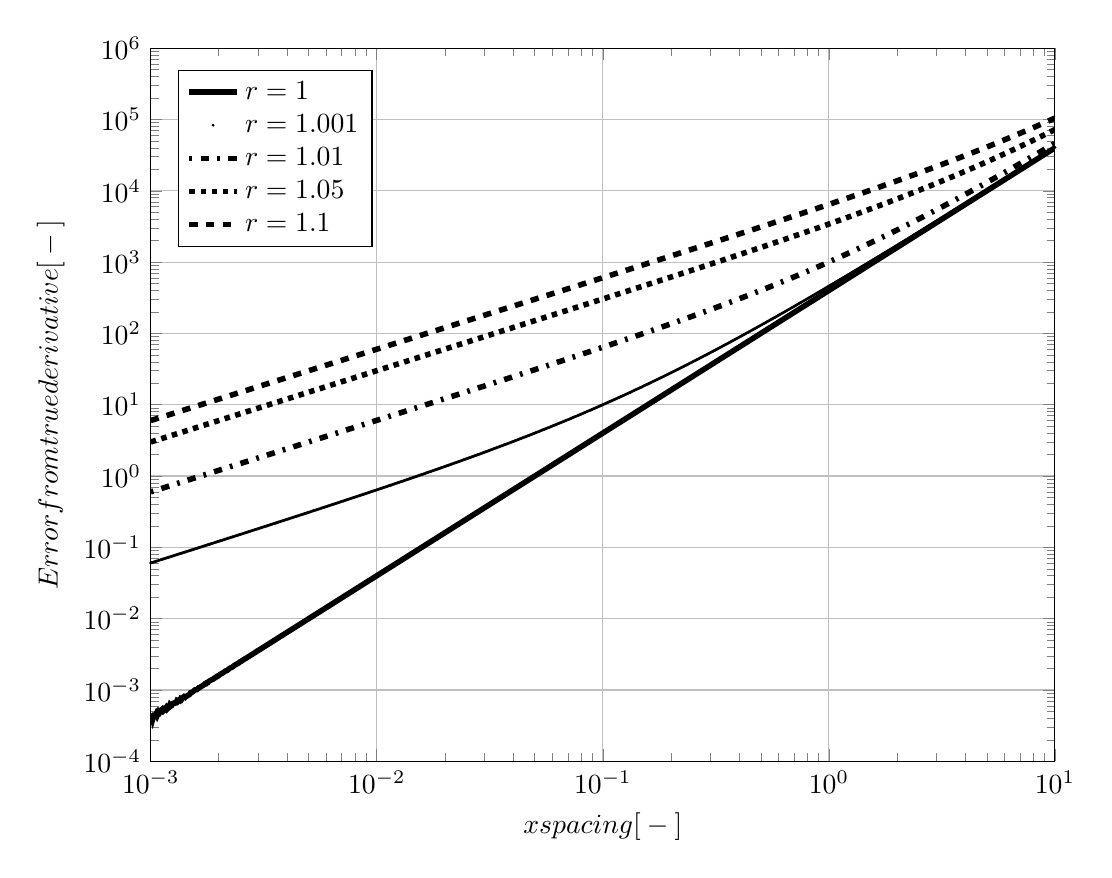
\begin{tikzpicture}

\begin{loglogaxis}[%
scale only axis,
width=4.52083in,
height=3.56562in,
xmin=0.001, xmax=10,
ymin=0.0001, ymax=1e+06,
xminorticks=true,
yminorticks=true,
xlabel={$\text{x spacing [}-\text{]}$},
ylabel={$\text{Error from true derivative [}-\text{]}$},
xmajorgrids,
ymajorgrids,
legend entries={$\text{r }= 1$,$\text{r }= 1.001$,$\text{r }= 1.01$,$\text{r }= 1.05$,$\text{r }= 1.1$},
legend style={at={(0.03,0.97)},anchor=north west,nodes=right}]
\addplot [
color=black,
solid,
line width=2.0pt
]
coordinates{
 (0.001,0.000417233)(0.00100926,0.000425701)(0.00101861,0.000386835)(0.00102804,0.000429543)(0.00103757,0.000432724)(0.00104718,0.000430804)(0.00105688,0.000459132)(0.00106666,0.00043322)(0.00107654,0.000461335)(0.00108652,0.000499934)(0.00109658,0.00048741)(0.00110674,0.000515447)(0.00111699,0.000528295)(0.00112733,0.000511887)(0.00113777,0.00053938)(0.00114831,0.00052622)(0.00115895,0.00054269)(0.00116968,0.000565593)(0.00118052,0.000537667)(0.00119145,0.000552793)(0.00120249,0.000570111)(0.00121362,0.000614056)(0.00122486,0.000590091)(0.00123621,0.000602316)(0.00124766,0.000630325)(0.00125922,0.00065311)(0.00127088,0.000658412)(0.00128265,0.000654965)(0.00129453,0.000658644)(0.00130652,0.000705488)(0.00131862,0.000692065)(0.00133083,0.000714908)(0.00134316,0.000706742)(0.0013556,0.000749638)(0.00136816,0.000737058)(0.00138083,0.000780313)(0.00139362,0.000783256)(0.00140653,0.000805786)(0.00141955,0.000791139)(0.0014327,0.000815265)(0.00144597,0.000820371)(0.00145937,0.000840547)(0.00147288,0.000853544)(0.00148652,0.000868803)(0.00150029,0.000913921)(0.00151419,0.000921059)(0.00152821,0.000934072)(0.00154237,0.000954158)(0.00155665,0.000982954)(0.00157107,0.00100397)(0.00158562,0.00100967)(0.00160031,0.00101074)(0.00161513,0.00103782)(0.00163009,0.00107215)(0.00164519,0.00107727)(0.00166043,0.00110292)(0.00167581,0.00112303)(0.00169133,0.00114434)(0.00170699,0.00116722)(0.00172281,0.00118497)(0.00173876,0.00122376)(0.00175487,0.00122087)(0.00177112,0.00126892)(0.00178753,0.00126924)(0.00180408,0.00131208)(0.00182079,0.00133802)(0.00183766,0.00136288)(0.00185468,0.00138257)(0.00187186,0.00140028)(0.00188919,0.0014181)(0.00190669,0.00145808)(0.00192435,0.00147902)(0.00194217,0.00150639)(0.00196016,0.00154765)(0.00197832,0.00155106)(0.00199664,0.00159576)(0.00201514,0.00162183)(0.0020338,0.00166703)(0.00205264,0.00168912)(0.00207165,0.00171555)(0.00209084,0.0017545)(0.0021102,0.00178603)(0.00212975,0.00182486)(0.00214947,0.00185946)(0.00216938,0.00186756)(0.00218948,0.00190685)(0.00220976,0.00195202)(0.00223022,0.00199902)(0.00225088,0.00203868)(0.00227173,0.00205895)(0.00229277,0.00209016)(0.00231401,0.00213906)(0.00233544,0.00218475)(0.00235707,0.00223565)(0.0023789,0.00226823)(0.00240093,0.00230634)(0.00242317,0.00234931)(0.00244562,0.0023777)(0.00246827,0.00244701)(0.00249113,0.00248959)(0.0025142,0.00252518)(0.00253749,0.00258154)(0.00256099,0.00262861)(0.00258471,0.00268106)(0.00260865,0.00272724)(0.00263282,0.00276719)(0.0026572,0.00282081)(0.00268181,0.00287504)(0.00270665,0.00293042)(0.00273172,0.00297748)(0.00275702,0.00304752)(0.00278256,0.003095)(0.00280833,0.0031545)(0.00283434,0.00320818)(0.0028606,0.00328193)(0.00288709,0.00332757)(0.00291383,0.0033903)(0.00294082,0.00346818)(0.00296806,0.00353255)(0.00299555,0.00358471)(0.00302329,0.00366287)(0.0030513,0.0037192)(0.00307956,0.00378919)(0.00310808,0.00386177)(0.00313687,0.00394396)(0.00316592,0.00400688)(0.00319525,0.00408136)(0.00322484,0.00416352)(0.00325471,0.00424213)(0.00328486,0.00431298)(0.00331528,0.00439013)(0.00334599,0.00447405)(0.00337698,0.00455221)(0.00340826,0.00464746)(0.00343983,0.00473808)(0.00347169,0.00482125)(0.00350384,0.00491766)(0.0035363,0.00499337)(0.00356905,0.00509016)(0.00360211,0.0051879)(0.00363547,0.00529128)(0.00366914,0.00538355)(0.00370313,0.00548701)(0.00373743,0.00558228)(0.00377204,0.0056994)(0.00380698,0.00579417)(0.00384224,0.00590418)(0.00387783,0.00601346)(0.00391375,0.00612381)(0.00395,0.00624833)(0.00398658,0.00635231)(0.00402351,0.00648021)(0.00406077,0.00659262)(0.00409838,0.00672047)(0.00413634,0.00684746)(0.00417466,0.00696583)(0.00421332,0.00710037)(0.00425235,0.00722873)(0.00429173,0.00736523)(0.00433148,0.00751032)(0.0043716,0.00763801)(0.00441209,0.00778622)(0.00445296,0.0079324)(0.0044942,0.00807569)(0.00453583,0.00822857)(0.00457784,0.00838045)(0.00462024,0.0085415)(0.00466303,0.00870346)(0.00470622,0.00885866)(0.00474981,0.00902828)(0.00479381,0.00919806)(0.00483821,0.00936285)(0.00488302,0.00953287)(0.00492825,0.00971602)(0.0049739,0.00989127)(0.00501997,0.0100836)(0.00506646,0.0102675)(0.00511339,0.0104604)(0.00516075,0.0106492)(0.00520855,0.0108573)(0.00525679,0.0110572)(0.00530548,0.011255)(0.00535462,0.0114664)(0.00540422,0.0116776)(0.00545427,0.0118954)(0.00550479,0.0121225)(0.00555578,0.0123428)(0.00560723,0.0125713)(0.00565917,0.0128058)(0.00571159,0.0130517)(0.00576449,0.0132872)(0.00581788,0.0135412)(0.00587177,0.0137954)(0.00592615,0.0140469)(0.00598104,0.0143108)(0.00603644,0.0145732)(0.00609235,0.0148431)(0.00614878,0.0151196)(0.00620573,0.0154039)(0.00626321,0.0156869)(0.00632122,0.0159866)(0.00637977,0.01628)(0.00643886,0.0165845)(0.0064985,0.0168881)(0.00655869,0.0172052)(0.00661943,0.0175312)(0.00668074,0.0178527)(0.00674262,0.0181827)(0.00680507,0.0185267)(0.0068681,0.0188709)(0.00693172,0.019223)(0.00699592,0.0195783)(0.00706072,0.0199439)(0.00712612,0.0203112)(0.00719212,0.0206941)(0.00725873,0.0210733)(0.00732597,0.0214646)(0.00739382,0.0218669)(0.0074623,0.0222776)(0.00753142,0.022689)(0.00760118,0.0231132)(0.00767158,0.0235422)(0.00774264,0.0239762)(0.00781435,0.0244262)(0.00788673,0.0248812)(0.00795978,0.0253425)(0.0080335,0.0258155)(0.00810791,0.0262916)(0.00818301,0.0267859)(0.0082588,0.0272843)(0.00833529,0.0277933)(0.0084125,0.0283063)(0.00849042,0.0288375)(0.00856906,0.029372)(0.00864842,0.0299179)(0.00872853,0.0304776)(0.00880937,0.0310434)(0.00889097,0.0316163)(0.00897332,0.0322096)(0.00905643,0.0328107)(0.00914031,0.0334212)(0.00922497,0.0340379)(0.00931041,0.0346746)(0.00939665,0.035322)(0.00948368,0.0359761)(0.00957152,0.0366436)(0.00966017,0.0373269)(0.00974965,0.0380244)(0.00983995,0.0387285)(0.00993109,0.0394533)(0.0100231,0.0401833)(0.0101159,0.0409343)(0.0102096,0.0416959)(0.0103042,0.0424705)(0.0103996,0.0432601)(0.0104959,0.0440676)(0.0105931,0.0448831)(0.0106913,0.0457213)(0.0107903,0.0465704)(0.0108902,0.0474366)(0.0109911,0.0483225)(0.0110929,0.0492211)(0.0111956,0.0501368)(0.0112993,0.0510688)(0.011404,0.0520183)(0.0115096,0.0529865)(0.0116162,0.0539735)(0.0117238,0.0549779)(0.0118324,0.0560007)(0.011942,0.0570456)(0.0120526,0.0581067)(0.0121642,0.0591854)(0.0122769,0.0602894)(0.0123906,0.0614115)(0.0125054,0.0625521)(0.0126212,0.0637178)(0.0127381,0.064903)(0.0128561,0.06611)(0.0129752,0.0673428)(0.0130954,0.0685938)(0.0132166,0.0698709)(0.0133391,0.0711728)(0.0134626,0.0724982)(0.0135873,0.0738441)(0.0137131,0.0752206)(0.0138402,0.076619)(0.0139684,0.0780454)(0.0140977,0.0794994)(0.0142283,0.0809778)(0.0143601,0.0824866)(0.0144931,0.0840195)(0.0146273,0.0855851)(0.0147628,0.0871754)(0.0148996,0.0887989)(0.0150376,0.0904494)(0.0151768,0.092133)(0.0153174,0.0938478)(0.0154593,0.0955973)(0.0156025,0.0973761)(0.015747,0.0991882)(0.0158928,0.101034)(0.01604,0.102914)(0.0161886,0.104829)(0.0163385,0.106779)(0.0164899,0.108767)(0.0166426,0.11079)(0.0167967,0.112851)(0.0169523,0.114952)(0.0171093,0.117092)(0.0172678,0.119271)(0.0174277,0.121492)(0.0175892,0.123751)(0.0177521,0.126054)(0.0179165,0.1284)(0.0180824,0.13079)(0.0182499,0.133223)(0.018419,0.135704)(0.0185896,0.138227)(0.0187617,0.140802)(0.0189355,0.143421)(0.0191109,0.146091)(0.0192879,0.148811)(0.0194666,0.15158)(0.0196469,0.154398)(0.0198288,0.157273)(0.0200125,0.160201)(0.0201979,0.16318)(0.0203849,0.166219)(0.0205737,0.169313)(0.0207643,0.172463)(0.0209566,0.175672)(0.0211507,0.178941)(0.0213466,0.182271)(0.0215443,0.185662)(0.0217439,0.189119)(0.0219453,0.192639)(0.0221486,0.196225)(0.0223537,0.199874)(0.0225607,0.203595)(0.0227697,0.207384)(0.0229806,0.211243)(0.0231935,0.215174)(0.0234083,0.219179)(0.0236251,0.223258)(0.0238439,0.227413)(0.0240648,0.231644)(0.0242876,0.235956)(0.0245126,0.240346)(0.0247396,0.244819)(0.0249688,0.249376)(0.0252,0.254017)(0.0254335,0.258745)(0.025669,0.26356)(0.0259068,0.268466)(0.0261467,0.27346)(0.0263889,0.278549)(0.0266333,0.283733)(0.02688,0.289014)(0.027129,0.294393)(0.0273803,0.299871)(0.0276339,0.305453)(0.0278898,0.311137)(0.0281481,0.316927)(0.0284088,0.322825)(0.028672,0.328832)(0.0289375,0.334951)(0.0292056,0.341187)(0.0294761,0.347536)(0.0297491,0.354002)(0.0300246,0.360592)(0.0303027,0.367302)(0.0305834,0.374138)(0.0308666,0.381101)(0.0311525,0.388193)(0.0314411,0.395416)(0.0317323,0.402774)(0.0320262,0.410271)(0.0323228,0.417906)(0.0326222,0.425683)(0.0329244,0.433606)(0.0332293,0.441675)(0.0335371,0.449895)(0.0338477,0.458268)(0.0341612,0.466797)(0.0344776,0.475484)(0.034797,0.484332)(0.0351193,0.493346)(0.0354446,0.502527)(0.0357729,0.511879)(0.0361042,0.521405)(0.0364386,0.531108)(0.0367761,0.540992)(0.0371167,0.55106)(0.0374605,0.561315)(0.0378075,0.571762)(0.0381576,0.582403)(0.0385111,0.593242)(0.0388678,0.604281)(0.0392278,0.615528)(0.0395911,0.626983)(0.0399578,0.63865)(0.0403279,0.650535)(0.0407014,0.662642)(0.0410784,0.674974)(0.0414589,0.687536)(0.0418429,0.700331)(0.0422304,0.713364)(0.0426216,0.726641)(0.0430164,0.740163)(0.0434148,0.753937)(0.0438169,0.767969)(0.0442227,0.782261)(0.0446323,0.796819)(0.0450457,0.811647)(0.045463,0.826752)(0.045884,0.842138)(0.046309,0.857811)(0.046738,0.873774)(0.0471708,0.890035)(0.0476078,0.9066)(0.0480487,0.923471)(0.0484937,0.940657)(0.0489429,0.958163)(0.0493962,0.975995)(0.0498537,0.994159)(0.0503155,1.01266)(0.0507815,1.03151)(0.0512519,1.0507)(0.0517266,1.07026)(0.0522057,1.09017)(0.0526892,1.11046)(0.0531772,1.13113)(0.0536698,1.15218)(0.0541669,1.17362)(0.0546686,1.19546)(0.0551749,1.21771)(0.055686,1.24037)(0.0562017,1.26345)(0.0567223,1.28697)(0.0572477,1.31092)(0.0577779,1.33531)(0.0583131,1.36016)(0.0588532,1.38548)(0.0593983,1.41126)(0.0599484,1.43753)(0.0605037,1.46428)(0.0610641,1.49153)(0.0616297,1.51929)(0.0622005,1.54756)(0.0627766,1.57636)(0.063358,1.6057)(0.0639449,1.63558)(0.0645372,1.66602)(0.0651349,1.69702)(0.0657382,1.7286)(0.0663471,1.76077)(0.0669616,1.79354)(0.0675818,1.82692)(0.0682078,1.86092)(0.0688395,1.89555)(0.0694771,1.93083)(0.0701206,1.96676)(0.0707701,2.00336)(0.0714256,2.04065)(0.0720872,2.07862)(0.0727548,2.11731)(0.0734287,2.15671)(0.0741088,2.19685)(0.0747952,2.23773)(0.075488,2.27937)(0.0761872,2.32179)(0.0768928,2.365)(0.077605,2.40902)(0.0783238,2.45385)(0.0790493,2.49952)(0.0797814,2.54603)(0.0805204,2.59341)(0.0812662,2.64168)(0.0820189,2.69084)(0.0827786,2.74092)(0.0835453,2.79193)(0.0843191,2.84388)(0.0851001,2.89681)(0.0858883,2.95072)(0.0866838,3.00563)(0.0874867,3.06157)(0.088297,3.11854)(0.0891148,3.17658)(0.0899402,3.2357)(0.0907733,3.29591)(0.091614,3.35725)(0.0924626,3.41973)(0.093319,3.48337)(0.0941833,3.5482)(0.0950557,3.61423)(0.0959361,3.68149)(0.0968247,3.75001)(0.0977215,3.81979)(0.0986266,3.89088)(0.0995401,3.96329)(0.100462,4.03705)(0.101393,4.11218)(0.102332,4.18871)(0.103279,4.26666)(0.104236,4.34606)(0.105202,4.42694)(0.106176,4.50933)(0.107159,4.59325)(0.108152,4.67873)(0.109154,4.7658)(0.110165,4.8545)(0.111185,4.94484)(0.112215,5.03686)(0.113254,5.1306)(0.114303,5.22608)(0.115362,5.32334)(0.11643,5.42241)(0.117509,5.52332)(0.118597,5.62611)(0.119696,5.73081)(0.120804,5.83746)(0.121923,5.9461)(0.123052,6.05676)(0.124192,6.16947)(0.125342,6.28429)(0.126503,6.40124)(0.127675,6.52037)(0.128858,6.64171)(0.130051,6.76532)(0.131256,6.89122)(0.132471,7.01947)(0.133698,7.1501)(0.134937,7.28317)(0.136187,7.41871)(0.137448,7.55677)(0.138721,7.6974)(0.140006,7.84065)(0.141303,7.98657)(0.142611,8.1352)(0.143932,8.2866)(0.145265,8.44081)(0.146611,8.5979)(0.147969,8.75791)(0.149339,8.92089)(0.150723,9.08691)(0.152119,9.25602)(0.153528,9.42828)(0.15495,9.60374)(0.156385,9.78247)(0.157833,9.96452)(0.159295,10.15)(0.16077,10.3389)(0.16226,10.5313)(0.163762,10.7273)(0.165279,10.9269)(0.16681,11.1302)(0.168355,11.3374)(0.169914,11.5484)(0.171488,11.7633)(0.173077,11.9822)(0.17468,12.2052)(0.176298,12.4323)(0.17793,12.6637)(0.179578,12.8994)(0.181242,13.1394)(0.18292,13.384)(0.184615,13.633)(0.186325,13.8867)(0.18805,14.1452)(0.189792,14.4084)(0.19155,14.6766)(0.193324,14.9497)(0.195115,15.2279)(0.196922,15.5113)(0.198746,15.8)(0.200587,16.094)(0.202445,16.3935)(0.20432,16.6986)(0.206212,17.0094)(0.208122,17.3259)(0.21005,17.6484)(0.211995,17.9768)(0.213959,18.3114)(0.215941,18.6521)(0.217941,18.9993)(0.219959,19.3528)(0.221997,19.713)(0.224053,20.0799)(0.226128,20.4536)(0.228222,20.8342)(0.230336,21.2219)(0.23247,21.6169)(0.234623,22.0192)(0.236796,22.4289)(0.238989,22.8463)(0.241203,23.2715)(0.243437,23.7046)(0.245692,24.1458)(0.247967,24.5951)(0.250264,25.0528)(0.252582,25.5191)(0.254921,25.994)(0.257283,26.4777)(0.259666,26.9705)(0.262071,27.4724)(0.264498,27.9837)(0.266948,28.5045)(0.26942,29.0349)(0.271916,29.5753)(0.274434,30.1257)(0.276976,30.6863)(0.279542,31.2574)(0.282131,31.8391)(0.284744,32.4316)(0.287381,33.0352)(0.290043,33.65)(0.292729,34.2762)(0.295441,34.9141)(0.298177,35.5639)(0.300939,36.2257)(0.303726,36.8999)(0.30654,37.5866)(0.309379,38.2861)(0.312244,38.9986)(0.315136,39.7244)(0.318055,40.4636)(0.321001,41.2167)(0.323974,41.9837)(0.326975,42.7651)(0.330003,43.5609)(0.33306,44.3716)(0.336145,45.1974)(0.339258,46.0385)(0.342401,46.8953)(0.345572,47.768)(0.348773,48.657)(0.352003,49.5625)(0.355263,50.4849)(0.358554,51.4244)(0.361875,52.3814)(0.365227,53.3562)(0.36861,54.3492)(0.372024,55.3606)(0.375469,56.3909)(0.378947,57.4404)(0.382457,58.5093)(0.385999,59.5982)(0.389575,60.7073)(0.393183,61.8371)(0.396825,62.9879)(0.4005,64.1601)(0.40421,65.3542)(0.407953,66.5704)(0.411732,67.8093)(0.415546,69.0712)(0.419394,70.3567)(0.423279,71.666)(0.427199,72.9997)(0.431156,74.3583)(0.43515,75.7421)(0.43918,77.1517)(0.443248,78.5875)(0.447353,80.05)(0.451497,81.5397)(0.455679,83.0572)(0.459899,84.6029)(0.464159,86.1774)(0.468458,87.7812)(0.472797,89.4148)(0.477176,91.0788)(0.481596,92.7738)(0.486056,94.5003)(0.490558,96.259)(0.495102,98.0504)(0.499688,99.8751)(0.504316,101.734)(0.508987,103.627)(0.513701,105.556)(0.518459,107.52)(0.523261,109.521)(0.528108,111.559)(0.532999,113.635)(0.537936,115.75)(0.542919,117.904)(0.547947,120.098)(0.553022,122.334)(0.558145,124.61)(0.563314,126.929)(0.568532,129.291)(0.573798,131.697)(0.579112,134.148)(0.584476,136.645)(0.58989,139.188)(0.595353,141.778)(0.600868,144.417)(0.606433,147.104)(0.61205,149.842)(0.617719,152.631)(0.62344,155.471)(0.629215,158.364)(0.635043,161.312)(0.640924,164.314)(0.646861,167.372)(0.652852,170.486)(0.658899,173.659)(0.665002,176.891)(0.671161,180.183)(0.677378,183.536)(0.683652,186.952)(0.689984,190.431)(0.696374,193.975)(0.702824,197.585)(0.709334,201.262)(0.715904,205.007)(0.722535,208.823)(0.729227,212.709)(0.735981,216.667)(0.742798,220.7)(0.749678,224.807)(0.756622,228.991)(0.76363,233.252)(0.770703,237.593)(0.777841,242.015)(0.785046,246.519)(0.792317,251.106)(0.799655,255.78)(0.807062,260.54)(0.814537,265.388)(0.822082,270.327)(0.829696,275.358)(0.837381,280.483)(0.845137,285.702)(0.852964,291.019)(0.860865,296.435)(0.868838,301.952)(0.876886,307.571)(0.885007,313.295)(0.893205,319.126)(0.901478,325.065)(0.909827,331.114)(0.918254,337.276)(0.926759,343.553)(0.935343,349.947)(0.944006,356.459)(0.95275,363.093)(0.961575,369.85)(0.970481,376.733)(0.97947,383.744)(0.988542,390.886)(0.997698,398.16)(1.00694,405.57)(1.01627,413.118)(1.02568,420.806)(1.03518,428.637)(1.04477,436.614)(1.05444,444.74)(1.06421,453.017)(1.07407,461.447)(1.08401,470.035)(1.09405,478.782)(1.10419,487.693)(1.11442,496.769)(1.12474,506.013)(1.13515,515.43)(1.14567,525.023)(1.15628,534.793)(1.16699,544.746)(1.1778,554.884)(1.18871,565.21)(1.19972,575.729)(1.21083,586.443)(1.22204,597.357)(1.23336,608.474)(1.24479,619.798)(1.25632,631.333)(1.26795,643.082)(1.2797,655.05)(1.29155,667.24)(1.30351,679.658)(1.31559,692.306)(1.32777,705.19)(1.34007,718.314)(1.35248,731.682)(1.36501,745.299)(1.37765,759.169)(1.39041,773.297)(1.40329,787.688)(1.41629,802.347)(1.4294,817.279)(1.44264,832.489)(1.45601,847.981)(1.46949,863.762)(1.4831,879.837)(1.49684,896.211)(1.5107,912.89)(1.5247,929.879)(1.53882,947.184)(1.55307,964.811)(1.56746,982.767)(1.58197,1001.06)(1.59663,1019.69)(1.61141,1038.66)(1.62634,1057.99)(1.6414,1077.68)(1.65661,1097.74)(1.67195,1118.17)(1.68744,1138.98)(1.70307,1160.17)(1.71884,1181.76)(1.73476,1203.76)(1.75083,1226.16)(1.76704,1248.98)(1.78341,1272.22)(1.79993,1295.9)(1.8166,1320.01)(1.83343,1344.58)(1.85041,1369.6)(1.86755,1395.09)(1.88484,1421.05)(1.9023,1447.5)(1.91992,1474.44)(1.9377,1501.88)(1.95565,1529.83)(1.97376,1558.3)(1.99205,1587.3)(2.0105,1616.84)(2.02912,1646.93)(2.04791,1677.58)(2.06688,1708.8)(2.08602,1740.6)(2.10535,1772.99)(2.12485,1805.99)(2.14453,1839.6)(2.16439,1873.83)(2.18444,1908.7)(2.20467,1944.23)(2.22509,1980.41)(2.2457,2017.26)(2.2665,2054.81)(2.28749,2093.05)(2.30868,2132)(2.33006,2171.67)(2.35164,2212.09)(2.37342,2253.26)(2.39541,2295.19)(2.41759,2337.9)(2.43999,2381.41)(2.46259,2425.73)(2.48539,2470.88)(2.50842,2516.86)(2.53165,2563.7)(2.5551,2611.41)(2.57876,2660.01)(2.60265,2709.51)(2.62675,2759.93)(2.65108,2811.3)(2.67564,2863.62)(2.70042,2916.91)(2.72543,2971.19)(2.75068,3026.49)(2.77615,3082.81)(2.80187,3140.18)(2.82782,3198.62)(2.85401,3258.15)(2.88044,3318.78)(2.90712,3380.55)(2.93405,3443.46)(2.96123,3507.54)(2.98865,3572.82)(3.01633,3639.31)(3.04427,3707.04)(3.07247,3776.03)(3.10093,3846.3)(3.12965,3917.88)(3.15864,3990.79)(3.18789,4065.06)(3.21742,4140.71)(3.24722,4217.77)(3.27729,4296.26)(3.30765,4376.22)(3.33829,4457.66)(3.36921,4540.62)(3.40041,4625.12)(3.43191,4711.19)(3.46369,4798.87)(3.49578,4888.18)(3.52815,4979.15)(3.56083,5071.81)(3.59381,5166.2)(3.6271,5262.34)(3.6607,5360.28)(3.6946,5460.03)(3.72882,5561.64)(3.76336,5665.15)(3.79822,5770.58)(3.8334,5877.97)(3.8689,5987.36)(3.90474,6098.78)(3.9409,6212.28)(3.9774,6327.89)(4.01424,6445.66)(4.05142,6565.61)(4.08895,6687.8)(4.12682,6812.26)(4.16504,6939.04)(4.20362,7068.17)(4.24256,7199.71)(4.28185,7333.7)(4.32151,7470.18)(4.36154,7609.2)(4.40194,7750.81)(4.44271,7895.06)(4.48386,8041.99)(4.52539,8191.65)(4.5673,8344.1)(4.6096,8499.38)(4.6523,8657.56)(4.69539,8818.67)(4.73888,8982.79)(4.78277,9149.96)(4.82707,9320.25)(4.87178,9493.7)(4.9169,9670.38)(4.96244,9850.34)(5.00841,10033.7)(5.0548,10220.4)(5.10162,10410.6)(5.14887,10604.3)(5.19656,10801.7)(5.24469,11002.7)(5.29327,11207.5)(5.34229,11416)(5.39177,11628.5)(5.44171,11844.9)(5.49212,12065.3)(5.54299,12289.9)(5.59433,12518.6)(5.64614,12751.6)(5.69844,12988.9)(5.75122,13230.6)(5.80449,13476.8)(5.85825,13727.6)(5.91251,13983.1)(5.96727,14243.3)(6.02254,14508.4)(6.07832,14778.4)(6.13462,15053.4)(6.19144,15333.6)(6.24879,15618.9)(6.30667,15909.6)(6.36508,16205.7)(6.42403,16507.3)(6.48353,16814.5)(6.54359,17127.4)(6.60419,17446.2)(6.66536,17770.8)(6.7271,18101.5)(6.78941,18438.4)(6.85229,18781.6)(6.91576,19131.1)(6.97981,19487.1)(7.04446,19849.8)(7.10971,20219.2)(7.17556,20595.5)(7.24202,20978.8)(7.3091,21369.2)(7.3768,21766.9)(7.44512,22171.9)(7.51408,22584.6)(7.58368,23004.9)(7.65392,23433)(7.72481,23869.1)(7.79636,24313.3)(7.86857,24765.8)(7.94145,25226.7)(8.01501,25696.1)(8.08924,26174.3)(8.16417,26661.5)(8.23979,27157.6)(8.3161,27663)(8.39313,28177.8)(8.47087,28702.2)(8.54933,29236.4)(8.62851,29780.5)(8.70843,30334.7)(8.78909,30899.2)(8.8705,31474.3)(8.95266,32060)(9.03558,32656.7)(9.11927,33264.4)(9.20373,33883.5)(9.28898,34514.1)(9.37502,35156.4)(9.46185,35810.6)(9.54949,36477.1)(9.63793,37155.9)(9.7272,37847.4)(9.8173,38551.7)(9.90823,39269.2)(10,40000) 
};

\addplot [
color=black,
mark size=0.3pt,
only marks,
mark=*,
mark options={solid}
]
coordinates{
 (0.001,0.0604089)(0.00100926,0.0609849)(0.00101861,0.0615158)(0.00102804,0.0621208)(0.00103757,0.062684)(0.00104718,0.0632663)(0.00105688,0.063879)(0.00106666,0.0644425)(0.00107654,0.0650482)(0.00108652,0.0656704)(0.00109658,0.0662708)(0.00110674,0.0669023)(0.00111699,0.0675308)(0.00112733,0.0681556)(0.00113777,0.0688028)(0.00114831,0.0694385)(0.00115895,0.0700903)(0.00116968,0.0707502)(0.00118052,0.0713799)(0.00119145,0.0720587)(0.00120249,0.0727239)(0.00121362,0.0734136)(0.00122486,0.074087)(0.00123621,0.0747713)(0.00124766,0.0754953)(0.00125922,0.076194)(0.00127088,0.0768927)(0.00128265,0.0776218)(0.00129453,0.078335)(0.00130652,0.0790969)(0.00131862,0.0798116)(0.00133083,0.0805632)(0.00134316,0.0813026)(0.0013556,0.0820823)(0.00136816,0.0828237)(0.00138083,0.083624)(0.00139362,0.0843966)(0.00140653,0.0851859)(0.00141955,0.0859846)(0.0014327,0.086788)(0.00144597,0.0875902)(0.00145937,0.0884054)(0.00147288,0.0892334)(0.00148652,0.0900707)(0.00150029,0.0909332)(0.00151419,0.0917717)(0.00152821,0.0926242)(0.00154237,0.0935059)(0.00155665,0.0943794)(0.00157107,0.0952665)(0.00158562,0.0961495)(0.00160031,0.097029)(0.00161513,0.0979442)(0.00163009,0.0988701)(0.00164519,0.0998001)(0.00166043,0.100727)(0.00167581,0.101674)(0.00169133,0.102623)(0.00170699,0.103593)(0.00172281,0.104554)(0.00173876,0.105541)(0.00175487,0.106522)(0.00177112,0.107533)(0.00178753,0.108528)(0.00180408,0.109545)(0.00182079,0.110583)(0.00183766,0.111623)(0.00185468,0.112668)(0.00187186,0.113709)(0.00188919,0.114767)(0.00190669,0.115861)(0.00192435,0.116951)(0.00194217,0.118032)(0.00196016,0.119155)(0.00197832,0.120261)(0.00199664,0.121398)(0.00201514,0.122531)(0.0020338,0.123689)(0.00205264,0.124853)(0.00207165,0.126013)(0.00209084,0.127199)(0.0021102,0.128396)(0.00212975,0.129613)(0.00214947,0.130824)(0.00216938,0.132035)(0.00218948,0.133287)(0.00220976,0.134542)(0.00223022,0.135804)(0.00225088,0.137087)(0.00227173,0.138368)(0.00229277,0.13967)(0.00231401,0.140985)(0.00233544,0.142314)(0.00235707,0.143654)(0.0023789,0.144994)(0.00240093,0.146363)(0.00242317,0.147737)(0.00244562,0.149121)(0.00246827,0.150542)(0.00249113,0.151954)(0.0025142,0.153377)(0.00253749,0.154828)(0.00256099,0.156288)(0.00258471,0.157761)(0.00260865,0.159249)(0.00263282,0.160742)(0.0026572,0.162256)(0.00268181,0.163782)(0.00270665,0.165332)(0.00273172,0.166889)(0.00275702,0.16847)(0.00278256,0.170055)(0.00280833,0.171656)(0.00283434,0.173274)(0.0028606,0.174916)(0.00288709,0.176554)(0.00291383,0.178228)(0.00294082,0.179919)(0.00296806,0.181609)(0.00299555,0.183325)(0.00302329,0.185062)(0.0030513,0.1868)(0.00307956,0.188565)(0.00310808,0.190355)(0.00313687,0.192156)(0.00316592,0.193966)(0.00319525,0.195797)(0.00322484,0.197661)(0.00325471,0.199527)(0.00328486,0.201411)(0.00331528,0.20331)(0.00334599,0.205243)(0.00337698,0.207181)(0.00340826,0.209149)(0.00343983,0.211132)(0.00347169,0.21313)(0.00350384,0.215148)(0.0035363,0.217182)(0.00356905,0.219246)(0.00360211,0.221318)(0.00363547,0.223428)(0.00366914,0.22554)(0.00370313,0.227676)(0.00373743,0.229834)(0.00377204,0.232024)(0.00380698,0.234222)(0.00384224,0.236446)(0.00387783,0.238692)(0.00391375,0.240953)(0.00395,0.243252)(0.00398658,0.245555)(0.00402351,0.247892)(0.00406077,0.250245)(0.00409838,0.25263)(0.00413634,0.255031)(0.00417466,0.257452)(0.00421332,0.259907)(0.00425235,0.262381)(0.00429173,0.264877)(0.00433148,0.2674)(0.0043716,0.269947)(0.00441209,0.272519)(0.00445296,0.275116)(0.0044942,0.277741)(0.00453583,0.280386)(0.00457784,0.283062)(0.00462024,0.285764)(0.00466303,0.288494)(0.00470622,0.291244)(0.00474981,0.294023)(0.00479381,0.296831)(0.00483821,0.299663)(0.00488302,0.302525)(0.00492825,0.305421)(0.0049739,0.308339)(0.00501997,0.31129)(0.00506646,0.314269)(0.00511339,0.317276)(0.00516075,0.320307)(0.00520855,0.323378)(0.00525679,0.326471)(0.00530548,0.329596)(0.00535462,0.332758)(0.00540422,0.335943)(0.00545427,0.339162)(0.00550479,0.342419)(0.00555578,0.345703)(0.00560723,0.349023)(0.00565917,0.352371)(0.00571159,0.35576)(0.00576449,0.359174)(0.00581788,0.362629)(0.00587177,0.366115)(0.00592615,0.36963)(0.00598104,0.373186)(0.00603644,0.376774)(0.00609235,0.380399)(0.00614878,0.384063)(0.00620573,0.387765)(0.00626321,0.391496)(0.00632122,0.395272)(0.00637977,0.399081)(0.00643886,0.402932)(0.0064985,0.406819)(0.00655869,0.410742)(0.00661943,0.414711)(0.00668074,0.418717)(0.00674262,0.422759)(0.00680507,0.426849)(0.0068681,0.430974)(0.00693172,0.435142)(0.00699592,0.439351)(0.00706072,0.443604)(0.00712612,0.4479)(0.00719212,0.452241)(0.00725873,0.456618)(0.00732597,0.461047)(0.00739382,0.46552)(0.0074623,0.470038)(0.00753142,0.474597)(0.00760118,0.479206)(0.00767158,0.48386)(0.00774264,0.488562)(0.00781435,0.493312)(0.00788673,0.498109)(0.00795978,0.502955)(0.0080335,0.507852)(0.00810791,0.512793)(0.00818301,0.517792)(0.0082588,0.522838)(0.00833529,0.527937)(0.0084125,0.533085)(0.00849042,0.53829)(0.00856906,0.543545)(0.00864842,0.548853)(0.00872853,0.55422)(0.00880937,0.559637)(0.00889097,0.565109)(0.00897332,0.57064)(0.00905643,0.576227)(0.00914031,0.581871)(0.00922497,0.587571)(0.00931041,0.593334)(0.00939665,0.599155)(0.00948368,0.605033)(0.00957152,0.610973)(0.00966017,0.616974)(0.00974965,0.623041)(0.00983995,0.629165)(0.00993109,0.635357)(0.0100231,0.64161)(0.0101159,0.64793)(0.0102096,0.654313)(0.0103042,0.660763)(0.0103996,0.66728)(0.0104959,0.673867)(0.0105931,0.680517)(0.0106913,0.687244)(0.0107903,0.694035)(0.0108902,0.7009)(0.0109911,0.707837)(0.0110929,0.714845)(0.0111956,0.721925)(0.0112993,0.72908)(0.011404,0.736311)(0.0115096,0.743617)(0.0116162,0.751002)(0.0117238,0.758462)(0.0118324,0.766003)(0.011942,0.773623)(0.0120526,0.781321)(0.0121642,0.7891)(0.0122769,0.796964)(0.0123906,0.804909)(0.0125054,0.812939)(0.0126212,0.821054)(0.0127381,0.829256)(0.0128561,0.837543)(0.0129752,0.84592)(0.0130954,0.854385)(0.0132166,0.86294)(0.0133391,0.871586)(0.0134626,0.880327)(0.0135873,0.889157)(0.0137131,0.898086)(0.0138402,0.907107)(0.0139684,0.916225)(0.0140977,0.925442)(0.0142283,0.934758)(0.0143601,0.944173)(0.0144931,0.95369)(0.0146273,0.96331)(0.0147628,0.973031)(0.0148996,0.982862)(0.0150376,0.992795)(0.0151768,1.00284)(0.0153174,1.01299)(0.0154593,1.02325)(0.0156025,1.03362)(0.015747,1.0441)(0.0158928,1.0547)(0.01604,1.06542)(0.0161886,1.07625)(0.0163385,1.0872)(0.0164899,1.09827)(0.0166426,1.10946)(0.0167967,1.12077)(0.0169523,1.13221)(0.0171093,1.14377)(0.0172678,1.15546)(0.0174277,1.16728)(0.0175892,1.17923)(0.0177521,1.1913)(0.0179165,1.20352)(0.0180824,1.21587)(0.0182499,1.22835)(0.018419,1.24098)(0.0185896,1.25374)(0.0187617,1.26665)(0.0189355,1.2797)(0.0191109,1.29289)(0.0192879,1.30623)(0.0194666,1.31972)(0.0196469,1.33336)(0.0198288,1.34716)(0.0200125,1.36111)(0.0201979,1.37522)(0.0203849,1.38948)(0.0205737,1.40391)(0.0207643,1.41849)(0.0209566,1.43325)(0.0211507,1.44816)(0.0213466,1.46325)(0.0215443,1.47851)(0.0217439,1.49394)(0.0219453,1.50955)(0.0221486,1.52533)(0.0223537,1.5413)(0.0225607,1.55744)(0.0227697,1.57377)(0.0229806,1.59029)(0.0231935,1.607)(0.0234083,1.62389)(0.0236251,1.64099)(0.0238439,1.65827)(0.0240648,1.67576)(0.0242876,1.69345)(0.0245126,1.71134)(0.0247396,1.72944)(0.0249688,1.74775)(0.0252,1.76627)(0.0254335,1.78501)(0.025669,1.80396)(0.0259068,1.82314)(0.0261467,1.84254)(0.0263889,1.86216)(0.0266333,1.88202)(0.02688,1.9021)(0.027129,1.92243)(0.0273803,1.94299)(0.0276339,1.96379)(0.0278898,1.98484)(0.0281481,2.00613)(0.0284088,2.02768)(0.028672,2.04948)(0.0289375,2.07154)(0.0292056,2.09386)(0.0294761,2.11645)(0.0297491,2.1393)(0.0300246,2.16243)(0.0303027,2.18583)(0.0305834,2.20952)(0.0308666,2.23348)(0.0311525,2.25773)(0.0314411,2.28228)(0.0317323,2.30712)(0.0320262,2.33225)(0.0323228,2.3577)(0.0326222,2.38344)(0.0329244,2.4095)(0.0332293,2.43588)(0.0335371,2.46257)(0.0338477,2.48959)(0.0341612,2.51694)(0.0344776,2.54462)(0.034797,2.57263)(0.0351193,2.601)(0.0354446,2.6297)(0.0357729,2.65876)(0.0361042,2.68818)(0.0364386,2.71796)(0.0367761,2.7481)(0.0371167,2.77862)(0.0374605,2.80951)(0.0378075,2.84078)(0.0381576,2.87244)(0.0385111,2.9045)(0.0388678,2.93695)(0.0392278,2.96981)(0.0395911,3.00308)(0.0399578,3.03676)(0.0403279,3.07086)(0.0407014,3.10539)(0.0410784,3.14035)(0.0414589,3.17576)(0.0418429,3.21161)(0.0422304,3.2479)(0.0426216,3.28466)(0.0430164,3.32189)(0.0434148,3.35958)(0.0438169,3.39775)(0.0442227,3.43641)(0.0446323,3.47556)(0.0450457,3.5152)(0.045463,3.55536)(0.045884,3.59602)(0.046309,3.63721)(0.046738,3.67893)(0.0471708,3.72118)(0.0476078,3.76397)(0.0480487,3.80732)(0.0484937,3.85122)(0.0489429,3.8957)(0.0493962,3.94074)(0.0498537,3.98638)(0.0503155,4.0326)(0.0507815,4.07943)(0.0512519,4.12687)(0.0517266,4.17492)(0.0522057,4.22361)(0.0526892,4.27293)(0.0531772,4.32289)(0.0536698,4.37352)(0.0541669,4.42481)(0.0546686,4.47677)(0.0551749,4.52942)(0.055686,4.58277)(0.0562017,4.63682)(0.0567223,4.69159)(0.0572477,4.74709)(0.0577779,4.80333)(0.0583131,4.86031)(0.0588532,4.91805)(0.0593983,4.97657)(0.0599484,5.03587)(0.0605037,5.09596)(0.0610641,5.15687)(0.0616297,5.21859)(0.0622005,5.28114)(0.0627766,5.34453)(0.063358,5.40879)(0.0639449,5.47391)(0.0645372,5.53992)(0.0651349,5.60682)(0.0657382,5.67463)(0.0663471,5.74336)(0.0669616,5.81303)(0.0675818,5.88366)(0.0682078,5.95525)(0.0688395,6.02782)(0.0694771,6.10139)(0.0701206,6.17597)(0.0707701,6.25158)(0.0714256,6.32823)(0.0720872,6.40593)(0.0727548,6.48472)(0.0734287,6.56459)(0.0741088,6.64558)(0.0747952,6.72768)(0.075488,6.81094)(0.0761872,6.89535)(0.0768928,6.98094)(0.077605,7.06773)(0.0783238,7.15574)(0.0790493,7.24497)(0.0797814,7.33547)(0.0805204,7.42723)(0.0812662,7.52029)(0.0820189,7.61467)(0.0827786,7.71038)(0.0835453,7.80744)(0.0843191,7.90588)(0.0851001,8.00571)(0.0858883,8.10697)(0.0866838,8.20967)(0.0874867,8.31383)(0.088297,8.41949)(0.0891148,8.52665)(0.0899402,8.63535)(0.0907733,8.74561)(0.091614,8.85746)(0.0924626,8.97091)(0.093319,9.086)(0.0941833,9.20275)(0.0950557,9.32119)(0.0959361,9.44134)(0.0968247,9.56324)(0.0977215,9.68691)(0.0986266,9.81237)(0.0995401,9.93967)(0.100462,10.0688)(0.101393,10.1998)(0.102332,10.3328)(0.103279,10.4677)(0.104236,10.6046)(0.105202,10.7435)(0.106176,10.8844)(0.107159,11.0274)(0.108152,11.1725)(0.109154,11.3198)(0.110165,11.4692)(0.111185,11.6209)(0.112215,11.7748)(0.113254,11.931)(0.114303,12.0895)(0.115362,12.2504)(0.11643,12.4137)(0.117509,12.5794)(0.118597,12.7476)(0.119696,12.9183)(0.120804,13.0916)(0.121923,13.2674)(0.123052,13.446)(0.124192,13.6272)(0.125342,13.8111)(0.126503,13.9979)(0.127675,14.1874)(0.128858,14.3798)(0.130051,14.5752)(0.131256,14.7735)(0.132471,14.9748)(0.133698,15.1792)(0.134937,15.3867)(0.136187,15.5973)(0.137448,15.8112)(0.138721,16.0284)(0.140006,16.2489)(0.141303,16.4727)(0.142611,16.7)(0.143932,16.9308)(0.145265,17.1652)(0.146611,17.4032)(0.147969,17.6448)(0.149339,17.8902)(0.150723,18.1394)(0.152119,18.3924)(0.153528,18.6494)(0.15495,18.9103)(0.156385,19.1753)(0.157833,19.4445)(0.159295,19.7178)(0.16077,19.9954)(0.16226,20.2774)(0.163762,20.5637)(0.165279,20.8546)(0.16681,21.15)(0.168355,21.45)(0.169914,21.7548)(0.171488,22.0644)(0.173077,22.3788)(0.17468,22.6982)(0.176298,23.0226)(0.17793,23.3522)(0.179578,23.687)(0.181242,24.0271)(0.18292,24.3726)(0.184615,24.7236)(0.186325,25.0801)(0.18805,25.4424)(0.189792,25.8104)(0.19155,26.1843)(0.193324,26.5641)(0.195115,26.9501)(0.196922,27.3422)(0.198746,27.7406)(0.200587,28.1454)(0.202445,28.5566)(0.20432,28.9745)(0.206212,29.3992)(0.208122,29.8306)(0.21005,30.269)(0.211995,30.7145)(0.213959,31.1672)(0.215941,31.6273)(0.217941,32.0947)(0.219959,32.5698)(0.221997,33.0525)(0.224053,33.5432)(0.226128,34.0417)(0.228222,34.5484)(0.230336,35.0634)(0.23247,35.5867)(0.234623,36.1186)(0.236796,36.6592)(0.238989,37.2086)(0.241203,37.767)(0.243437,38.3346)(0.245692,38.9115)(0.247967,39.4978)(0.250264,40.0938)(0.252582,40.6996)(0.254921,41.3153)(0.257283,41.9412)(0.259666,42.5775)(0.262071,43.2242)(0.264498,43.8816)(0.266948,44.5499)(0.26942,45.2293)(0.271916,45.9199)(0.274434,46.6219)(0.276976,47.3357)(0.279542,48.0612)(0.282131,48.7989)(0.284744,49.5488)(0.287381,50.3112)(0.290043,51.0863)(0.292729,51.8743)(0.295441,52.6756)(0.298177,53.4902)(0.300939,54.3184)(0.303726,55.1605)(0.30654,56.0166)(0.309379,56.8872)(0.312244,57.7724)(0.315136,58.6724)(0.318055,59.5875)(0.321001,60.5181)(0.323974,61.4643)(0.326975,62.4264)(0.330003,63.4048)(0.33306,64.3997)(0.336145,65.4114)(0.339258,66.4402)(0.342401,67.4863)(0.345572,68.5502)(0.348773,69.6321)(0.352003,70.7324)(0.355263,71.8513)(0.358554,72.9892)(0.361875,74.1464)(0.365227,75.3233)(0.36861,76.5203)(0.372024,77.7376)(0.375469,78.9756)(0.378947,80.2348)(0.382457,81.5154)(0.385999,82.8179)(0.389575,84.1427)(0.393183,85.4901)(0.396825,86.8606)(0.4005,88.2545)(0.40421,89.6723)(0.407953,91.1144)(0.411732,92.5812)(0.415546,94.0733)(0.419394,95.5909)(0.423279,97.1346)(0.427199,98.7049)(0.431156,100.302)(0.43515,101.927)(0.43918,103.58)(0.443248,105.261)(0.447353,106.971)(0.451497,108.711)(0.455679,110.481)(0.459899,112.282)(0.464159,114.113)(0.468458,115.977)(0.472797,117.872)(0.477176,119.801)(0.481596,121.763)(0.486056,123.759)(0.490558,125.789)(0.495102,127.855)(0.499688,129.957)(0.504316,132.095)(0.508987,134.27)(0.513701,136.484)(0.518459,138.736)(0.523261,141.027)(0.528108,143.358)(0.532999,145.729)(0.537936,148.142)(0.542919,150.598)(0.547947,153.096)(0.553022,155.638)(0.558145,158.224)(0.563314,160.855)(0.568532,163.533)(0.573798,166.258)(0.579112,169.03)(0.584476,171.851)(0.58989,174.721)(0.595353,177.642)(0.600868,180.614)(0.606433,183.638)(0.61205,186.715)(0.617719,189.847)(0.62344,193.034)(0.629215,196.276)(0.635043,199.576)(0.640924,202.934)(0.646861,206.351)(0.652852,209.829)(0.658899,213.367)(0.665002,216.969)(0.671161,220.634)(0.677378,224.363)(0.683652,228.159)(0.689984,232.021)(0.696374,235.952)(0.702824,239.953)(0.709334,244.024)(0.715904,248.168)(0.722535,252.385)(0.729227,256.676)(0.735981,261.044)(0.742798,265.489)(0.749678,270.014)(0.756622,274.618)(0.76363,279.304)(0.770703,284.074)(0.777841,288.928)(0.785046,293.869)(0.792317,298.898)(0.799655,304.016)(0.807062,309.225)(0.814537,314.527)(0.822082,319.924)(0.829696,325.417)(0.837381,331.007)(0.845137,336.698)(0.852964,342.49)(0.860865,348.385)(0.868838,354.386)(0.876886,360.494)(0.885007,366.711)(0.893205,373.039)(0.901478,379.48)(0.909827,386.037)(0.918254,392.711)(0.926759,399.504)(0.935343,406.419)(0.944006,413.458)(0.95275,420.623)(0.961575,427.917)(0.970481,435.341)(0.97947,442.899)(0.988542,450.592)(0.997698,458.423)(1.00694,466.395)(1.01627,474.509)(1.02568,482.77)(1.03518,491.179)(1.04477,499.74)(1.05444,508.454)(1.06421,517.325)(1.07407,526.356)(1.08401,535.549)(1.09405,544.907)(1.10419,554.435)(1.11442,564.133)(1.12474,574.007)(1.13515,584.059)(1.14567,594.291)(1.15628,604.709)(1.16699,615.314)(1.1778,626.111)(1.18871,637.102)(1.19972,648.292)(1.21083,659.684)(1.22204,671.282)(1.23336,683.089)(1.24479,695.11)(1.25632,707.347)(1.26795,719.807)(1.2797,732.491)(1.29155,745.405)(1.30351,758.553)(1.31559,771.939)(1.32777,785.567)(1.34007,799.442)(1.35248,813.568)(1.36501,827.95)(1.37765,842.593)(1.39041,857.501)(1.40329,872.679)(1.41629,888.133)(1.4294,903.867)(1.44264,919.887)(1.45601,936.197)(1.46949,952.803)(1.4831,969.711)(1.49684,986.925)(1.5107,1004.45)(1.5247,1022.3)(1.53882,1040.47)(1.55307,1058.97)(1.56746,1077.81)(1.58197,1096.98)(1.59663,1116.51)(1.61141,1136.4)(1.62634,1156.64)(1.6414,1177.25)(1.65661,1198.24)(1.67195,1219.61)(1.68744,1241.37)(1.70307,1263.53)(1.71884,1286.09)(1.73476,1309.06)(1.75083,1332.45)(1.76704,1356.26)(1.78341,1380.51)(1.79993,1405.2)(1.8166,1430.34)(1.83343,1455.94)(1.85041,1482.01)(1.86755,1508.55)(1.88484,1535.58)(1.9023,1563.1)(1.91992,1591.12)(1.9377,1619.66)(1.95565,1648.71)(1.97376,1678.3)(1.99205,1708.43)(2.0105,1739.1)(2.02912,1770.34)(2.04791,1802.15)(2.06688,1834.54)(2.08602,1867.52)(2.10535,1901.11)(2.12485,1935.3)(2.14453,1970.13)(2.16439,2005.59)(2.18444,2041.7)(2.20467,2078.47)(2.22509,2115.92)(2.2457,2154.05)(2.2665,2192.88)(2.28749,2232.41)(2.30868,2272.68)(2.33006,2313.68)(2.35164,2355.43)(2.37342,2397.94)(2.39541,2441.24)(2.41759,2485.33)(2.43999,2530.23)(2.46259,2575.94)(2.48539,2622.5)(2.50842,2669.91)(2.53165,2718.2)(2.5551,2767.36)(2.57876,2817.43)(2.60265,2868.42)(2.62675,2920.34)(2.65108,2973.21)(2.67564,3027.06)(2.70042,3081.89)(2.72543,3137.73)(2.75068,3194.6)(2.77615,3252.51)(2.80187,3311.48)(2.82782,3371.54)(2.85401,3432.7)(2.88044,3494.98)(2.90712,3558.41)(2.93405,3623)(2.96123,3688.78)(2.98865,3755.77)(3.01633,3823.99)(3.04427,3893.46)(3.07247,3964.21)(3.10093,4036.26)(3.12965,4109.64)(3.15864,4184.37)(3.18789,4260.47)(3.21742,4337.97)(3.24722,4416.89)(3.27729,4497.27)(3.30765,4579.13)(3.33829,4662.49)(3.36921,4747.39)(3.40041,4833.85)(3.43191,4921.91)(3.46369,5011.58)(3.49578,5102.9)(3.52815,5195.91)(3.56083,5290.63)(3.59381,5387.09)(3.6271,5485.33)(3.6607,5585.38)(3.6946,5687.27)(3.72882,5791.04)(3.76336,5896.73)(3.79822,6004.35)(3.8334,6113.97)(3.8689,6225.6)(3.90474,6339.29)(3.9409,6455.08)(3.9774,6573)(4.01424,6693.09)(4.05142,6815.4)(4.08895,6939.97)(4.12682,7066.83)(4.16504,7196.03)(4.20362,7327.62)(4.24256,7461.63)(4.28185,7598.11)(4.32151,7737.11)(4.36154,7878.68)(4.40194,8022.86)(4.44271,8169.7)(4.48386,8319.25)(4.52539,8471.56)(4.5673,8626.68)(4.6096,8784.66)(4.6523,8945.56)(4.69539,9109.43)(4.73888,9276.33)(4.78277,9446.31)(4.82707,9619.42)(4.87178,9795.74)(4.9169,9975.31)(4.96244,10158.2)(5.00841,10344.5)(5.0548,10534.2)(5.10162,10727.4)(5.14887,10924.2)(5.19656,11124.6)(5.24469,11328.7)(5.29327,11536.6)(5.34229,11748.3)(5.39177,11964)(5.44171,12183.6)(5.49212,12407.3)(5.54299,12635.1)(5.59433,12867.1)(5.64614,13103.5)(5.69844,13344.2)(5.75122,13589.3)(5.80449,13839)(5.85825,14093.3)(5.91251,14352.3)(5.96727,14616)(6.02254,14884.7)(6.07832,15158.3)(6.13462,15437)(6.19144,15720.9)(6.24879,16010)(6.30667,16304.4)(6.36508,16604.3)(6.42403,16909.8)(6.48353,17220.9)(6.54359,17537.7)(6.60419,17860.4)(6.66536,18189.1)(6.7271,18523.9)(6.78941,18864.9)(6.85229,19212.1)(6.91576,19565.8)(6.97981,19926.1)(7.04446,20293)(7.10971,20666.7)(7.17556,21047.4)(7.24202,21435)(7.3091,21829.9)(7.3768,22232.1)(7.44512,22641.7)(7.51408,23058.9)(7.58368,23483.8)(7.65392,23916.6)(7.72481,24357.4)(7.79636,24806.4)(7.86857,25263.6)(7.94145,25729.4)(8.01501,26203.8)(8.08924,26687)(8.16417,27179.1)(8.23979,27680.3)(8.3161,28190.8)(8.39313,28710.8)(8.47087,29240.4)(8.54933,29779.9)(8.62851,30329.3)(8.70843,30888.9)(8.78909,31458.9)(8.8705,32039.4)(8.95266,32630.7)(9.03558,33233)(9.11927,33846.4)(9.20373,34471.2)(9.28898,35107.5)(9.37502,35755.7)(9.46185,36415.9)(9.54949,37088.3)(9.63793,37773.2)(9.7272,38470.8)(9.8173,39181.3)(9.90823,39904.9)(10,40642) 
};

\addplot [
color=black,
dash pattern=on 1pt off 3pt on 3pt off 3pt,
line width=2.0pt
]
coordinates{
 (0.001,0.600398)(0.00100926,0.60598)(0.00101861,0.61156)(0.00102804,0.617248)(0.00103757,0.62298)(0.00104718,0.62874)(0.00105688,0.634575)(0.00106666,0.64044)(0.00107654,0.646413)(0.00108652,0.652384)(0.00109658,0.658439)(0.00110674,0.664553)(0.00111699,0.670699)(0.00112733,0.676919)(0.00113777,0.683206)(0.00114831,0.689507)(0.00115895,0.695924)(0.00116968,0.702362)(0.00118052,0.708859)(0.00119145,0.715434)(0.00120249,0.722059)(0.00121362,0.728795)(0.00122486,0.735524)(0.00123621,0.742348)(0.00124766,0.749237)(0.00125922,0.756171)(0.00127088,0.763175)(0.00128265,0.770258)(0.00129453,0.777392)(0.00130652,0.784616)(0.00131862,0.791887)(0.00133083,0.799227)(0.00134316,0.806617)(0.0013556,0.814109)(0.00136816,0.82164)(0.00138083,0.829287)(0.00139362,0.83696)(0.00140653,0.844713)(0.00141955,0.852541)(0.0014327,0.860444)(0.00144597,0.868428)(0.00145937,0.87647)(0.00147288,0.884591)(0.00148652,0.892804)(0.00150029,0.901088)(0.00151419,0.909452)(0.00152821,0.917868)(0.00154237,0.926384)(0.00155665,0.934975)(0.00157107,0.943651)(0.00158562,0.952388)(0.00160031,0.961212)(0.00161513,0.970127)(0.00163009,0.979129)(0.00164519,0.988206)(0.00166043,0.997371)(0.00167581,1.00662)(0.00169133,1.01595)(0.00170699,1.02537)(0.00172281,1.03488)(0.00173876,1.04449)(0.00175487,1.05417)(0.00177112,1.06394)(0.00178753,1.0738)(0.00180408,1.08377)(0.00182079,1.09382)(0.00183766,1.10396)(0.00185468,1.1142)(0.00187186,1.12453)(0.00188919,1.13495)(0.00190669,1.14549)(0.00192435,1.15611)(0.00194217,1.16683)(0.00196016,1.17765)(0.00197832,1.18856)(0.00199664,1.1996)(0.00201514,1.21071)(0.0020338,1.22196)(0.00205264,1.23329)(0.00207165,1.24473)(0.00209084,1.25627)(0.0021102,1.26792)(0.00212975,1.27968)(0.00214947,1.29156)(0.00216938,1.30353)(0.00218948,1.31561)(0.00220976,1.32782)(0.00223022,1.34015)(0.00225088,1.35258)(0.00227173,1.36513)(0.00229277,1.37778)(0.00231401,1.39056)(0.00233544,1.40347)(0.00235707,1.4165)(0.0023789,1.42962)(0.00240093,1.44288)(0.00242317,1.45628)(0.00244562,1.46978)(0.00246827,1.48342)(0.00249113,1.49719)(0.0025142,1.51107)(0.00253749,1.5251)(0.00256099,1.53925)(0.00258471,1.55353)(0.00260865,1.56794)(0.00263282,1.58249)(0.0026572,1.59717)(0.00268181,1.612)(0.00270665,1.62695)(0.00273172,1.64205)(0.00275702,1.65729)(0.00278256,1.67266)(0.00280833,1.68819)(0.00283434,1.70384)(0.0028606,1.71967)(0.00288709,1.73562)(0.00291383,1.75173)(0.00294082,1.76799)(0.00296806,1.7844)(0.00299555,1.80095)(0.00302329,1.81768)(0.0030513,1.83453)(0.00307956,1.85157)(0.00310808,1.86875)(0.00313687,1.8861)(0.00316592,1.9036)(0.00319525,1.92127)(0.00322484,1.93911)(0.00325471,1.95711)(0.00328486,1.97527)(0.00331528,1.99361)(0.00334599,2.01212)(0.00337698,2.03079)(0.00340826,2.04965)(0.00343983,2.06868)(0.00347169,2.08788)(0.00350384,2.10727)(0.0035363,2.12682)(0.00356905,2.14657)(0.00360211,2.16651)(0.00363547,2.18663)(0.00366914,2.20692)(0.00370313,2.22742)(0.00373743,2.2481)(0.00377204,2.26898)(0.00380698,2.29004)(0.00384224,2.31131)(0.00387783,2.33277)(0.00391375,2.35444)(0.00395,2.37631)(0.00398658,2.39836)(0.00402351,2.42064)(0.00406077,2.44313)(0.00409838,2.46582)(0.00413634,2.48872)(0.00417466,2.51183)(0.00421332,2.53516)(0.00425235,2.55871)(0.00429173,2.58248)(0.00433148,2.60647)(0.0043716,2.63068)(0.00441209,2.65512)(0.00445296,2.67979)(0.0044942,2.70468)(0.00453583,2.72981)(0.00457784,2.75517)(0.00462024,2.78077)(0.00466303,2.80661)(0.00470622,2.83268)(0.00474981,2.859)(0.00479381,2.88557)(0.00483821,2.91238)(0.00488302,2.93945)(0.00492825,2.96676)(0.0049739,2.99433)(0.00501997,3.02216)(0.00506646,3.05025)(0.00511339,3.0786)(0.00516075,3.10721)(0.00520855,3.13609)(0.00525679,3.16524)(0.00530548,3.19466)(0.00535462,3.22436)(0.00540422,3.25433)(0.00545427,3.28458)(0.00550479,3.31512)(0.00555578,3.34593)(0.00560723,3.37704)(0.00565917,3.40844)(0.00571159,3.44013)(0.00576449,3.47211)(0.00581788,3.5044)(0.00587177,3.53699)(0.00592615,3.56988)(0.00598104,3.60308)(0.00603644,3.63658)(0.00609235,3.67041)(0.00614878,3.70454)(0.00620573,3.739)(0.00626321,3.77377)(0.00632122,3.80888)(0.00637977,3.84431)(0.00643886,3.88007)(0.0064985,3.91616)(0.00655869,3.95259)(0.00661943,3.98936)(0.00668074,4.02648)(0.00674262,4.06394)(0.00680507,4.10176)(0.0068681,4.13992)(0.00693172,4.17845)(0.00699592,4.21733)(0.00706072,4.25657)(0.00712612,4.29619)(0.00719212,4.33617)(0.00725873,4.37653)(0.00732597,4.41726)(0.00739382,4.45838)(0.0074623,4.49988)(0.00753142,4.54177)(0.00760118,4.58405)(0.00767158,4.62673)(0.00774264,4.6698)(0.00781435,4.71328)(0.00788673,4.75717)(0.00795978,4.80146)(0.0080335,4.84618)(0.00810791,4.89131)(0.00818301,4.93686)(0.0082588,4.98284)(0.00833529,5.02925)(0.0084125,5.07609)(0.00849042,5.12338)(0.00856906,5.1711)(0.00864842,5.21927)(0.00872853,5.2679)(0.00880937,5.31698)(0.00889097,5.36652)(0.00897332,5.41652)(0.00905643,5.467)(0.00914031,5.51794)(0.00922497,5.56936)(0.00931041,5.62127)(0.00939665,5.67367)(0.00948368,5.72655)(0.00957152,5.77993)(0.00966017,5.83381)(0.00974965,5.8882)(0.00983995,5.94309)(0.00993109,5.9985)(0.0100231,6.05444)(0.0101159,6.11089)(0.0102096,6.16788)(0.0103042,6.2254)(0.0103996,6.28346)(0.0104959,6.34207)(0.0105931,6.40123)(0.0106913,6.46094)(0.0107903,6.52121)(0.0108902,6.58205)(0.0109911,6.64347)(0.0110929,6.70546)(0.0111956,6.76803)(0.0112993,6.83119)(0.011404,6.89494)(0.0115096,6.9593)(0.0116162,7.02426)(0.0117238,7.08983)(0.0118324,7.15601)(0.011942,7.22282)(0.0120526,7.29026)(0.0121642,7.35833)(0.0122769,7.42705)(0.0123906,7.4964)(0.0125054,7.56642)(0.0126212,7.63709)(0.0127381,7.70843)(0.0128561,7.78044)(0.0129752,7.85313)(0.0130954,7.9265)(0.0132166,8.00056)(0.0133391,8.07533)(0.0134626,8.15079)(0.0135873,8.22697)(0.0137131,8.30387)(0.0138402,8.38149)(0.0139684,8.45984)(0.0140977,8.53894)(0.0142283,8.61878)(0.0143601,8.69937)(0.0144931,8.78073)(0.0146273,8.86285)(0.0147628,8.94574)(0.0148996,9.02943)(0.0150376,9.11389)(0.0151768,9.19916)(0.0153174,9.28524)(0.0154593,9.37213)(0.0156025,9.45984)(0.015747,9.54838)(0.0158928,9.63775)(0.01604,9.72797)(0.0161886,9.81905)(0.0163385,9.91098)(0.0164899,10.0038)(0.0166426,10.0975)(0.0167967,10.192)(0.0169523,10.2875)(0.0171093,10.3839)(0.0172678,10.4812)(0.0174277,10.5794)(0.0175892,10.6785)(0.0177521,10.7786)(0.0179165,10.8796)(0.0180824,10.9816)(0.0182499,11.0845)(0.018419,11.1885)(0.0185896,11.2934)(0.0187617,11.3993)(0.0189355,11.5062)(0.0191109,11.6141)(0.0192879,11.7231)(0.0194666,11.833)(0.0196469,11.9441)(0.0198288,12.0562)(0.0200125,12.1693)(0.0201979,12.2835)(0.0203849,12.3989)(0.0205737,12.5153)(0.0207643,12.6328)(0.0209566,12.7514)(0.0211507,12.8712)(0.0213466,12.9921)(0.0215443,13.1141)(0.0217439,13.2374)(0.0219453,13.3618)(0.0221486,13.4873)(0.0223537,13.6141)(0.0225607,13.7421)(0.0227697,13.8713)(0.0229806,14.0017)(0.0231935,14.1334)(0.0234083,14.2664)(0.0236251,14.4006)(0.0238439,14.5361)(0.0240648,14.6728)(0.0242876,14.8109)(0.0245126,14.9503)(0.0247396,15.0911)(0.0249688,15.2332)(0.0252,15.3766)(0.0254335,15.5214)(0.025669,15.6676)(0.0259068,15.8152)(0.0261467,15.9643)(0.0263889,16.1147)(0.0266333,16.2666)(0.02688,16.4199)(0.027129,16.5748)(0.0273803,16.7311)(0.0276339,16.8888)(0.0278898,17.0482)(0.0281481,17.209)(0.0284088,17.3714)(0.028672,17.5353)(0.0289375,17.7009)(0.0292056,17.868)(0.0294761,18.0367)(0.0297491,18.207)(0.0300246,18.379)(0.0303027,18.5526)(0.0305834,18.7279)(0.0308666,18.9049)(0.0311525,19.0836)(0.0314411,19.2641)(0.0317323,19.4462)(0.0320262,19.6301)(0.0323228,19.8158)(0.0326222,20.0033)(0.0329244,20.1926)(0.0332293,20.3837)(0.0335371,20.5767)(0.0338477,20.7715)(0.0341612,20.9683)(0.0344776,21.1669)(0.034797,21.3674)(0.0351193,21.5699)(0.0354446,21.7743)(0.0357729,21.9808)(0.0361042,22.1892)(0.0364386,22.3996)(0.0367761,22.6121)(0.0371167,22.8267)(0.0374605,23.0433)(0.0378075,23.262)(0.0381576,23.4829)(0.0385111,23.7059)(0.0388678,23.931)(0.0392278,24.1584)(0.0395911,24.388)(0.0399578,24.6198)(0.0403279,24.8538)(0.0407014,25.0902)(0.0410784,25.3288)(0.0414589,25.5698)(0.0418429,25.8131)(0.0422304,26.0588)(0.0426216,26.3069)(0.0430164,26.5575)(0.0434148,26.8104)(0.0438169,27.0659)(0.0442227,27.3238)(0.0446323,27.5843)(0.0450457,27.8473)(0.045463,28.1129)(0.045884,28.3811)(0.046309,28.6519)(0.046738,28.9254)(0.0471708,29.2015)(0.0476078,29.4804)(0.0480487,29.762)(0.0484937,30.0464)(0.0489429,30.3336)(0.0493962,30.6236)(0.0498537,30.9164)(0.0503155,31.2122)(0.0507815,31.5108)(0.0512519,31.8124)(0.0517266,32.117)(0.0522057,32.4246)(0.0526892,32.7352)(0.0531772,33.0489)(0.0536698,33.3657)(0.0541669,33.6856)(0.0546686,34.0087)(0.0551749,34.335)(0.055686,34.6645)(0.0562017,34.9973)(0.0567223,35.3333)(0.0572477,35.6728)(0.0577779,36.0155)(0.0583131,36.3617)(0.0588532,36.7114)(0.0593983,37.0645)(0.0599484,37.4211)(0.0605037,37.7813)(0.0610641,38.145)(0.0616297,38.5124)(0.0622005,38.8835)(0.0627766,39.2582)(0.063358,39.6367)(0.0639449,40.019)(0.0645372,40.4051)(0.0651349,40.7951)(0.0657382,41.189)(0.0663471,41.5868)(0.0669616,41.9886)(0.0675818,42.3945)(0.0682078,42.8044)(0.0688395,43.2184)(0.0694771,43.6366)(0.0701206,44.059)(0.0707701,44.4857)(0.0714256,44.9166)(0.0720872,45.3519)(0.0727548,45.7916)(0.0734287,46.2357)(0.0741088,46.6843)(0.0747952,47.1375)(0.075488,47.5952)(0.0761872,48.0576)(0.0768928,48.5246)(0.077605,48.9964)(0.0783238,49.4729)(0.0790493,49.9543)(0.0797814,50.4406)(0.0805204,50.9319)(0.0812662,51.4281)(0.0820189,51.9294)(0.0827786,52.4358)(0.0835453,52.9473)(0.0843191,53.4641)(0.0851001,53.9861)(0.0858883,54.5135)(0.0866838,55.0463)(0.0874867,55.5845)(0.088297,56.1283)(0.0891148,56.6776)(0.0899402,57.2325)(0.0907733,57.7932)(0.091614,58.3596)(0.0924626,58.9318)(0.093319,59.51)(0.0941833,60.094)(0.0950557,60.6841)(0.0959361,61.2803)(0.0968247,61.8827)(0.0977215,62.4913)(0.0986266,63.1061)(0.0995401,63.7274)(0.100462,64.3551)(0.101393,64.9893)(0.102332,65.63)(0.103279,66.2775)(0.104236,66.9316)(0.105202,67.5926)(0.106176,68.2604)(0.107159,68.9353)(0.108152,69.6171)(0.109154,70.3061)(0.110165,71.0023)(0.111185,71.7058)(0.112215,72.4166)(0.113254,73.1349)(0.114303,73.8608)(0.115362,74.5942)(0.11643,75.3354)(0.117509,76.0844)(0.118597,76.8412)(0.119696,77.6061)(0.120804,78.379)(0.121923,79.1601)(0.123052,79.9494)(0.124192,80.7471)(0.125342,81.5533)(0.126503,82.368)(0.127675,83.1913)(0.128858,84.0234)(0.130051,84.8644)(0.131256,85.7143)(0.132471,86.5733)(0.133698,87.4414)(0.134937,88.3188)(0.136187,89.2056)(0.137448,90.1019)(0.138721,91.0078)(0.140006,91.9234)(0.141303,92.8489)(0.142611,93.7842)(0.143932,94.7297)(0.145265,95.6854)(0.146611,96.6513)(0.147969,97.6277)(0.149339,98.6147)(0.150723,99.6123)(0.152119,100.621)(0.153528,101.64)(0.15495,102.671)(0.156385,103.712)(0.157833,104.765)(0.159295,105.83)(0.16077,106.906)(0.16226,107.993)(0.163762,109.093)(0.165279,110.205)(0.16681,111.329)(0.168355,112.465)(0.169914,113.614)(0.171488,114.775)(0.173077,115.949)(0.17468,117.136)(0.176298,118.337)(0.17793,119.55)(0.179578,120.777)(0.181242,122.017)(0.18292,123.272)(0.184615,124.54)(0.186325,125.822)(0.18805,127.118)(0.189792,128.429)(0.19155,129.755)(0.193324,131.095)(0.195115,132.451)(0.196922,133.821)(0.198746,135.207)(0.200587,136.609)(0.202445,138.026)(0.20432,139.459)(0.206212,140.909)(0.208122,142.374)(0.21005,143.857)(0.211995,145.356)(0.213959,146.872)(0.215941,148.405)(0.217941,149.956)(0.219959,151.524)(0.221997,153.11)(0.224053,154.715)(0.226128,156.337)(0.228222,157.978)(0.230336,159.638)(0.23247,161.317)(0.234623,163.016)(0.236796,164.733)(0.238989,166.471)(0.241203,168.229)(0.243437,170.006)(0.245692,171.805)(0.247967,173.624)(0.250264,175.465)(0.252582,177.326)(0.254921,179.21)(0.257283,181.115)(0.259666,183.043)(0.262071,184.993)(0.264498,186.966)(0.266948,188.961)(0.26942,190.981)(0.271916,193.024)(0.274434,195.091)(0.276976,197.182)(0.279542,199.299)(0.282131,201.44)(0.284744,203.606)(0.287381,205.798)(0.290043,208.016)(0.292729,210.261)(0.295441,212.532)(0.298177,214.83)(0.300939,217.156)(0.303726,219.509)(0.30654,221.891)(0.309379,224.301)(0.312244,226.74)(0.315136,229.208)(0.318055,231.706)(0.321001,234.234)(0.323974,236.793)(0.326975,239.383)(0.330003,242.004)(0.33306,244.657)(0.336145,247.342)(0.339258,250.059)(0.342401,252.81)(0.345572,255.594)(0.348773,258.413)(0.352003,261.266)(0.355263,264.154)(0.358554,267.077)(0.361875,270.036)(0.365227,273.032)(0.36861,276.065)(0.372024,279.135)(0.375469,282.243)(0.378947,285.39)(0.382457,288.576)(0.385999,291.801)(0.389575,295.066)(0.393183,298.373)(0.396825,301.72)(0.4005,305.109)(0.40421,308.541)(0.407953,312.016)(0.411732,315.535)(0.415546,319.098)(0.419394,322.705)(0.423279,326.359)(0.427199,330.058)(0.431156,333.805)(0.43515,337.599)(0.43918,341.441)(0.443248,345.332)(0.447353,349.272)(0.451497,353.263)(0.455679,357.305)(0.459899,361.399)(0.464159,365.545)(0.468458,369.745)(0.472797,373.998)(0.477176,378.307)(0.481596,382.671)(0.486056,387.091)(0.490558,391.569)(0.495102,396.104)(0.499688,400.699)(0.504316,405.354)(0.508987,410.069)(0.513701,414.845)(0.518459,419.684)(0.523261,424.587)(0.528108,429.554)(0.532999,434.586)(0.537936,439.684)(0.542919,444.849)(0.547947,450.083)(0.553022,455.386)(0.558145,460.759)(0.563314,466.203)(0.568532,471.72)(0.573798,477.31)(0.579112,482.975)(0.584476,488.715)(0.58989,494.532)(0.595353,500.426)(0.600868,506.4)(0.606433,512.454)(0.61205,518.59)(0.617719,524.808)(0.62344,531.11)(0.629215,537.498)(0.635043,543.972)(0.640924,550.533)(0.646861,557.184)(0.652852,563.925)(0.658899,570.758)(0.665002,577.685)(0.671161,584.706)(0.677378,591.823)(0.683652,599.037)(0.689984,606.351)(0.696374,613.766)(0.702824,621.282)(0.709334,628.902)(0.715904,636.628)(0.722535,644.46)(0.729227,652.401)(0.735981,660.453)(0.742798,668.616)(0.749678,676.893)(0.756622,685.285)(0.76363,693.795)(0.770703,702.424)(0.777841,711.173)(0.785046,720.046)(0.792317,729.043)(0.799655,738.167)(0.807062,747.419)(0.814537,756.802)(0.822082,766.318)(0.829696,775.968)(0.837381,785.756)(0.845137,795.682)(0.852964,805.75)(0.860865,815.961)(0.868838,826.318)(0.876886,836.823)(0.885007,847.478)(0.893205,858.286)(0.901478,869.249)(0.909827,880.37)(0.918254,891.651)(0.926759,903.095)(0.935343,914.704)(0.944006,926.48)(0.95275,938.428)(0.961575,950.548)(0.970481,962.845)(0.97947,975.321)(0.988542,987.978)(0.997698,1000.82)(1.00694,1013.85)(1.01627,1027.07)(1.02568,1040.48)(1.03518,1054.1)(1.04477,1067.91)(1.05444,1081.92)(1.06421,1096.14)(1.07407,1110.57)(1.08401,1125.22)(1.09405,1140.08)(1.10419,1155.16)(1.11442,1170.46)(1.12474,1186)(1.13515,1201.76)(1.14567,1217.76)(1.15628,1233.99)(1.16699,1250.47)(1.1778,1267.2)(1.18871,1284.18)(1.19972,1301.41)(1.21083,1318.9)(1.22204,1336.65)(1.23336,1354.68)(1.24479,1372.97)(1.25632,1391.54)(1.26795,1410.39)(1.2797,1429.53)(1.29155,1448.95)(1.30351,1468.67)(1.31559,1488.7)(1.32777,1509.02)(1.34007,1529.66)(1.35248,1550.61)(1.36501,1571.88)(1.37765,1593.48)(1.39041,1615.41)(1.40329,1637.67)(1.41629,1660.28)(1.4294,1683.24)(1.44264,1706.54)(1.45601,1730.21)(1.46949,1754.25)(1.4831,1778.65)(1.49684,1803.43)(1.5107,1828.6)(1.5247,1854.16)(1.53882,1880.11)(1.55307,1906.47)(1.56746,1933.24)(1.58197,1960.43)(1.59663,1988.04)(1.61141,2016.09)(1.62634,2044.57)(1.6414,2073.5)(1.65661,2102.88)(1.67195,2132.72)(1.68744,2163.04)(1.70307,2193.83)(1.71884,2225.11)(1.73476,2256.88)(1.75083,2289.15)(1.76704,2321.93)(1.78341,2355.23)(1.79993,2389.06)(1.8166,2423.43)(1.83343,2458.34)(1.85041,2493.81)(1.86755,2529.84)(1.88484,2566.45)(1.9023,2603.64)(1.91992,2641.43)(1.9377,2679.82)(1.95565,2718.82)(1.97376,2758.45)(1.99205,2798.72)(2.0105,2839.63)(2.02912,2881.2)(2.04791,2923.44)(2.06688,2966.36)(2.08602,3009.98)(2.10535,3054.29)(2.12485,3099.33)(2.14453,3145.09)(2.16439,3191.6)(2.18444,3238.85)(2.20467,3286.88)(2.22509,3335.69)(2.2457,3385.29)(2.2665,3435.69)(2.28749,3486.92)(2.30868,3538.99)(2.33006,3591.9)(2.35164,3645.68)(2.37342,3700.34)(2.39541,3755.89)(2.41759,3812.36)(2.43999,3869.75)(2.46259,3928.08)(2.48539,3987.38)(2.50842,4047.65)(2.53165,4108.91)(2.5551,4171.18)(2.57876,4234.48)(2.60265,4298.82)(2.62675,4364.23)(2.65108,4430.72)(2.67564,4498.31)(2.70042,4567.02)(2.72543,4636.87)(2.75068,4707.88)(2.77615,4780.07)(2.80187,4853.46)(2.82782,4928.08)(2.85401,5003.93)(2.88044,5081.05)(2.90712,5159.46)(2.93405,5239.18)(2.96123,5320.23)(2.98865,5402.63)(3.01633,5486.42)(3.04427,5571.61)(3.07247,5658.23)(3.10093,5746.3)(3.12965,5835.86)(3.15864,5926.92)(3.18789,6019.51)(3.21742,6113.66)(3.24722,6209.39)(3.27729,6306.74)(3.30765,6405.74)(3.33829,6506.41)(3.36921,6608.78)(3.40041,6712.88)(3.43191,6818.74)(3.46369,6926.4)(3.49578,7035.88)(3.52815,7147.22)(3.56083,7260.45)(3.59381,7375.6)(3.6271,7492.72)(3.6607,7611.82)(3.6946,7732.96)(3.72882,7856.16)(3.76336,7981.46)(3.79822,8108.89)(3.8334,8238.51)(3.8689,8370.34)(3.90474,8504.42)(3.9409,8640.8)(3.9774,8779.52)(4.01424,8920.61)(4.05142,9064.12)(4.08895,9210.1)(4.12682,9358.58)(4.16504,9509.61)(4.20362,9663.24)(4.24256,9819.51)(4.28185,9978.47)(4.32151,10140.2)(4.36154,10304.7)(4.40194,10472)(4.44271,10642.2)(4.48386,10815.3)(4.52539,10991.5)(4.5673,11170.7)(4.6096,11353)(4.6523,11538.4)(4.69539,11727.1)(4.73888,11919)(4.78277,12114.3)(4.82707,12312.9)(4.87178,12515)(4.9169,12720.6)(4.96244,12929.8)(5.00841,13142.6)(5.0548,13359.1)(5.10162,13579.4)(5.14887,13803.5)(5.19656,14031.5)(5.24469,14263.6)(5.29327,14499.6)(5.34229,14739.8)(5.39177,14984.2)(5.44171,15232.8)(5.49212,15485.8)(5.54299,15743.2)(5.59433,16005.2)(5.64614,16271.7)(5.69844,16542.9)(5.75122,16818.8)(5.80449,17099.6)(5.85825,17385.3)(5.91251,17676)(5.96727,17971.8)(6.02254,18272.9)(6.07832,18579.2)(6.13462,18890.9)(6.19144,19208.1)(6.24879,19530.9)(6.30667,19859.4)(6.36508,20193.6)(6.42403,20533.8)(6.48353,20879.9)(6.54359,21232.2)(6.60419,21590.7)(6.66536,21955.5)(6.7271,22326.8)(6.78941,22704.6)(6.85229,23089.1)(6.91576,23480.4)(6.97981,23878.7)(7.04446,24284)(7.10971,24696.5)(7.17556,25116.3)(7.24202,25543.5)(7.3091,25978.3)(7.3768,26420.9)(7.44512,26871.3)(7.51408,27329.7)(7.58368,27796.2)(7.65392,28271.1)(7.72481,28754.4)(7.79636,29246.2)(7.86857,29746.9)(7.94145,30256.4)(8.01501,30775.1)(8.08924,31302.9)(8.16417,31840.2)(8.23979,32387.1)(8.3161,32943.7)(8.39313,33510.3)(8.47087,34086.9)(8.54933,34673.9)(8.62851,35271.4)(8.70843,35879.5)(8.78909,36498.5)(8.8705,37128.6)(8.95266,37769.9)(9.03558,38422.8)(9.11927,39087.3)(9.20373,39763.7)(9.28898,40452.2)(9.37502,41153.1)(9.46185,41866.5)(9.54949,42592.8)(9.63793,43332)(9.7272,44084.6)(9.8173,44850.6)(9.90823,45630.4)(10,46424.2) 
};

\addplot [
color=black,
dotted,
line width=2.0pt
]
coordinates{
 (0.001,3.00044)(0.00100926,3.02822)(0.00101861,3.05624)(0.00102804,3.0846)(0.00103757,3.11315)(0.00104718,3.14198)(0.00105688,3.17111)(0.00106666,3.20046)(0.00107654,3.23013)(0.00108652,3.26005)(0.00109658,3.29026)(0.00110674,3.32074)(0.00111699,3.35151)(0.00112733,3.38253)(0.00113777,3.41387)(0.00114831,3.4455)(0.00115895,3.47741)(0.00116968,3.50964)(0.00118052,3.54212)(0.00119145,3.57494)(0.00120249,3.60807)(0.00121362,3.6415)(0.00122486,3.67521)(0.00123621,3.70927)(0.00124766,3.74364)(0.00125922,3.77833)(0.00127088,3.81332)(0.00128265,3.84865)(0.00129453,3.8843)(0.00130652,3.92029)(0.00131862,3.9566)(0.00133083,3.99325)(0.00134316,4.03024)(0.0013556,4.06759)(0.00136816,4.10525)(0.00138083,4.14331)(0.00139362,4.18167)(0.00140653,4.22043)(0.00141955,4.2595)(0.0014327,4.29898)(0.00144597,4.33878)(0.00145937,4.379)(0.00147288,4.41954)(0.00148652,4.4605)(0.00150029,4.50183)(0.00151419,4.54353)(0.00152821,4.58562)(0.00154237,4.62812)(0.00155665,4.671)(0.00157107,4.71427)(0.00158562,4.75793)(0.00160031,4.802)(0.00161513,4.84649)(0.00163009,4.89141)(0.00164519,4.93671)(0.00166043,4.98244)(0.00167581,5.02862)(0.00169133,5.07519)(0.00170699,5.12221)(0.00172281,5.16967)(0.00173876,5.21757)(0.00175487,5.26589)(0.00177112,5.31469)(0.00178753,5.36392)(0.00180408,5.41361)(0.00182079,5.46378)(0.00183766,5.51439)(0.00185468,5.56548)(0.00187186,5.61703)(0.00188919,5.66908)(0.00190669,5.72161)(0.00192435,5.77461)(0.00194217,5.82812)(0.00196016,5.88211)(0.00197832,5.9366)(0.00199664,5.9916)(0.00201514,6.04712)(0.0020338,6.10315)(0.00205264,6.15968)(0.00207165,6.21676)(0.00209084,6.27436)(0.0021102,6.33248)(0.00212975,6.39116)(0.00214947,6.45037)(0.00216938,6.51012)(0.00218948,6.57044)(0.00220976,6.63133)(0.00223022,6.69277)(0.00225088,6.75479)(0.00227173,6.81736)(0.00229277,6.88051)(0.00231401,6.94426)(0.00233544,7.00861)(0.00235707,7.07356)(0.0023789,7.13909)(0.00240093,7.20523)(0.00242317,7.272)(0.00244562,7.33936)(0.00246827,7.40738)(0.00249113,7.47601)(0.0025142,7.54527)(0.00253749,7.61518)(0.00256099,7.68574)(0.00258471,7.75696)(0.00260865,7.82883)(0.00263282,7.90137)(0.0026572,7.97458)(0.00268181,8.04846)(0.00270665,8.12304)(0.00273172,8.19831)(0.00275702,8.27427)(0.00278256,8.35094)(0.00280833,8.42832)(0.00283434,8.50641)(0.0028606,8.58524)(0.00288709,8.66478)(0.00291383,8.74507)(0.00294082,8.8261)(0.00296806,8.90789)(0.00299555,8.99042)(0.00302329,9.07374)(0.0030513,9.15781)(0.00307956,9.24267)(0.00310808,9.32831)(0.00313687,9.41476)(0.00316592,9.50199)(0.00319525,9.59004)(0.00322484,9.67891)(0.00325471,9.7686)(0.00328486,9.85911)(0.00331528,9.95048)(0.00334599,10.0427)(0.00337698,10.1357)(0.00340826,10.2297)(0.00343983,10.3245)(0.00347169,10.4201)(0.00350384,10.5167)(0.0035363,10.6141)(0.00356905,10.7125)(0.00360211,10.8118)(0.00363547,10.912)(0.00366914,11.0131)(0.00370313,11.1152)(0.00373743,11.2182)(0.00377204,11.3221)(0.00380698,11.427)(0.00384224,11.5329)(0.00387783,11.6398)(0.00391375,11.7477)(0.00395,11.8566)(0.00398658,11.9664)(0.00402351,12.0773)(0.00406077,12.1893)(0.00409838,12.3022)(0.00413634,12.4162)(0.00417466,12.5313)(0.00421332,12.6474)(0.00425235,12.7647)(0.00429173,12.8829)(0.00433148,13.0023)(0.0043716,13.1228)(0.00441209,13.2445)(0.00445296,13.3672)(0.0044942,13.4911)(0.00453583,13.6161)(0.00457784,13.7423)(0.00462024,13.8697)(0.00466303,13.9983)(0.00470622,14.128)(0.00474981,14.2589)(0.00479381,14.3911)(0.00483821,14.5245)(0.00488302,14.6591)(0.00492825,14.795)(0.0049739,14.9321)(0.00501997,15.0705)(0.00506646,15.2102)(0.00511339,15.3512)(0.00516075,15.4935)(0.00520855,15.6371)(0.00525679,15.782)(0.00530548,15.9283)(0.00535462,16.0759)(0.00540422,16.2249)(0.00545427,16.3753)(0.00550479,16.5271)(0.00555578,16.6803)(0.00560723,16.8349)(0.00565917,16.991)(0.00571159,17.1485)(0.00576449,17.3075)(0.00581788,17.4679)(0.00587177,17.6298)(0.00592615,17.7932)(0.00598104,17.9582)(0.00603644,18.1247)(0.00609235,18.2927)(0.00614878,18.4623)(0.00620573,18.6334)(0.00626321,18.8061)(0.00632122,18.9805)(0.00637977,19.1564)(0.00643886,19.334)(0.0064985,19.5133)(0.00655869,19.6942)(0.00661943,19.8768)(0.00668074,20.061)(0.00674262,20.247)(0.00680507,20.4347)(0.0068681,20.6242)(0.00693172,20.8154)(0.00699592,21.0084)(0.00706072,21.2031)(0.00712612,21.3997)(0.00719212,21.5981)(0.00725873,21.7984)(0.00732597,22.0005)(0.00739382,22.2045)(0.0074623,22.4104)(0.00753142,22.6181)(0.00760118,22.8279)(0.00767158,23.0395)(0.00774264,23.2531)(0.00781435,23.4688)(0.00788673,23.6864)(0.00795978,23.906)(0.0080335,24.1277)(0.00810791,24.3514)(0.00818301,24.5772)(0.0082588,24.8051)(0.00833529,25.0351)(0.0084125,25.2673)(0.00849042,25.5016)(0.00856906,25.7381)(0.00864842,25.9768)(0.00872853,26.2177)(0.00880937,26.4608)(0.00889097,26.7062)(0.00897332,26.9538)(0.00905643,27.2038)(0.00914031,27.4561)(0.00922497,27.7107)(0.00931041,27.9677)(0.00939665,28.2271)(0.00948368,28.4889)(0.00957152,28.7531)(0.00966017,29.0198)(0.00974965,29.289)(0.00983995,29.5606)(0.00993109,29.8348)(0.0100231,30.1115)(0.0101159,30.3908)(0.0102096,30.6727)(0.0103042,30.9572)(0.0103996,31.2444)(0.0104959,31.5342)(0.0105931,31.8267)(0.0106913,32.1219)(0.0107903,32.4199)(0.0108902,32.7206)(0.0109911,33.0242)(0.0110929,33.3305)(0.0111956,33.6397)(0.0112993,33.9518)(0.011404,34.2667)(0.0115096,34.5846)(0.0116162,34.9055)(0.0117238,35.2293)(0.0118324,35.5562)(0.011942,35.886)(0.0120526,36.219)(0.0121642,36.555)(0.0122769,36.8942)(0.0123906,37.2365)(0.0125054,37.582)(0.0126212,37.9307)(0.0127381,38.2827)(0.0128561,38.6379)(0.0129752,38.9964)(0.0130954,39.3582)(0.0132166,39.7235)(0.0133391,40.0921)(0.0134626,40.4641)(0.0135873,40.8396)(0.0137131,41.2186)(0.0138402,41.6011)(0.0139684,41.9872)(0.0140977,42.3769)(0.0142283,42.7701)(0.0143601,43.1671)(0.0144931,43.5677)(0.0146273,43.9721)(0.0147628,44.3802)(0.0148996,44.7921)(0.0150376,45.2079)(0.0151768,45.6275)(0.0153174,46.051)(0.0154593,46.4784)(0.0156025,46.9099)(0.015747,47.3453)(0.0158928,47.7848)(0.01604,48.2284)(0.0161886,48.6761)(0.0163385,49.128)(0.0164899,49.5841)(0.0166426,50.0444)(0.0167967,50.509)(0.0169523,50.978)(0.0171093,51.4513)(0.0172678,51.929)(0.0174277,52.4111)(0.0175892,52.8977)(0.0177521,53.3889)(0.0179165,53.8847)(0.0180824,54.385)(0.0182499,54.89)(0.018419,55.3997)(0.0185896,55.9142)(0.0187617,56.4334)(0.0189355,56.9575)(0.0191109,57.4865)(0.0192879,58.0204)(0.0194666,58.5592)(0.0196469,59.1031)(0.0198288,59.652)(0.0200125,60.2061)(0.0201979,60.7653)(0.0203849,61.3297)(0.0205737,61.8994)(0.0207643,62.4744)(0.0209566,63.0548)(0.0211507,63.6405)(0.0213466,64.2317)(0.0215443,64.8285)(0.0217439,65.4307)(0.0219453,66.0386)(0.0221486,66.6522)(0.0223537,67.2715)(0.0225607,67.8965)(0.0227697,68.5274)(0.0229806,69.1641)(0.0231935,69.8068)(0.0234083,70.4555)(0.0236251,71.1102)(0.0238439,71.7711)(0.0240648,72.4381)(0.0242876,73.1113)(0.0245126,73.7908)(0.0247396,74.4766)(0.0249688,75.1688)(0.0252,75.8675)(0.0254335,76.5727)(0.025669,77.2845)(0.0259068,78.0029)(0.0261467,78.728)(0.0263889,79.4599)(0.0266333,80.1986)(0.02688,80.9442)(0.027129,81.6968)(0.0273803,82.4564)(0.0276339,83.223)(0.0278898,83.9969)(0.0281481,84.7779)(0.0284088,85.5663)(0.028672,86.362)(0.0289375,87.1651)(0.0292056,87.9758)(0.0294761,88.794)(0.0297491,89.6198)(0.0300246,90.4534)(0.0303027,91.2947)(0.0305834,92.1439)(0.0308666,93.0011)(0.0311525,93.8662)(0.0314411,94.7394)(0.0317323,95.6208)(0.0320262,96.5104)(0.0323228,97.4084)(0.0326222,98.3147)(0.0329244,99.2295)(0.0332293,100.153)(0.0335371,101.085)(0.0338477,102.026)(0.0341612,102.975)(0.0344776,103.933)(0.034797,104.901)(0.0351193,105.877)(0.0354446,106.863)(0.0357729,107.857)(0.0361042,108.861)(0.0364386,109.875)(0.0367761,110.898)(0.0371167,111.93)(0.0374605,112.972)(0.0378075,114.024)(0.0381576,115.086)(0.0385111,116.158)(0.0388678,117.239)(0.0392278,118.331)(0.0395911,119.433)(0.0399578,120.546)(0.0403279,121.668)(0.0407014,122.802)(0.0410784,123.946)(0.0414589,125.1)(0.0418429,126.266)(0.0422304,127.442)(0.0426216,128.63)(0.0430164,129.828)(0.0434148,131.038)(0.0438169,132.259)(0.0442227,133.492)(0.0446323,134.736)(0.0450457,135.991)(0.045463,137.259)(0.045884,138.538)(0.046309,139.83)(0.046738,141.134)(0.0471708,142.449)(0.0476078,143.777)(0.0480487,145.118)(0.0484937,146.471)(0.0489429,147.837)(0.0493962,149.216)(0.0498537,150.608)(0.0503155,152.012)(0.0507815,153.43)(0.0512519,154.861)(0.0517266,156.306)(0.0522057,157.764)(0.0526892,159.236)(0.0531772,160.722)(0.0536698,162.222)(0.0541669,163.736)(0.0546686,165.264)(0.0551749,166.806)(0.055686,168.363)(0.0562017,169.935)(0.0567223,171.521)(0.0572477,173.123)(0.0577779,174.739)(0.0583131,176.371)(0.0588532,178.018)(0.0593983,179.68)(0.0599484,181.358)(0.0605037,183.052)(0.0610641,184.762)(0.0616297,186.488)(0.0622005,188.23)(0.0627766,189.989)(0.063358,191.764)(0.0639449,193.556)(0.0645372,195.365)(0.0651349,197.191)(0.0657382,199.034)(0.0663471,200.894)(0.0669616,202.773)(0.0675818,204.668)(0.0682078,206.582)(0.0688395,208.514)(0.0694771,210.464)(0.0701206,212.432)(0.0707701,214.419)(0.0714256,216.425)(0.0720872,218.449)(0.0727548,220.493)(0.0734287,222.556)(0.0741088,224.639)(0.0747952,226.741)(0.075488,228.863)(0.0761872,231.005)(0.0768928,233.168)(0.077605,235.351)(0.0783238,237.554)(0.0790493,239.779)(0.0797814,242.024)(0.0805204,244.291)(0.0812662,246.579)(0.0820189,248.889)(0.0827786,251.221)(0.0835453,253.574)(0.0843191,255.951)(0.0851001,258.349)(0.0858883,260.771)(0.0866838,263.215)(0.0874867,265.682)(0.088297,268.173)(0.0891148,270.688)(0.0899402,273.226)(0.0907733,275.789)(0.091614,278.376)(0.0924626,280.987)(0.093319,283.623)(0.0941833,286.285)(0.0950557,288.971)(0.0959361,291.683)(0.0968247,294.421)(0.0977215,297.185)(0.0986266,299.975)(0.0995401,302.792)(0.100462,305.635)(0.101393,308.506)(0.102332,311.404)(0.103279,314.329)(0.104236,317.283)(0.105202,320.264)(0.106176,323.274)(0.107159,326.313)(0.108152,329.38)(0.109154,332.477)(0.110165,335.603)(0.111185,338.759)(0.112215,341.946)(0.113254,345.163)(0.114303,348.41)(0.115362,351.688)(0.11643,354.998)(0.117509,358.34)(0.118597,361.713)(0.119696,365.119)(0.120804,368.557)(0.121923,372.028)(0.123052,375.532)(0.124192,379.07)(0.125342,382.642)(0.126503,386.248)(0.127675,389.888)(0.128858,393.563)(0.130051,397.274)(0.131256,401.02)(0.132471,404.802)(0.133698,408.621)(0.134937,412.476)(0.136187,416.368)(0.137448,420.298)(0.138721,424.265)(0.140006,428.27)(0.141303,432.314)(0.142611,436.397)(0.143932,440.519)(0.145265,444.68)(0.146611,448.882)(0.147969,453.124)(0.149339,457.408)(0.150723,461.732)(0.152119,466.098)(0.153528,470.506)(0.15495,474.957)(0.156385,479.45)(0.157833,483.987)(0.159295,488.568)(0.16077,493.193)(0.16226,497.863)(0.163762,502.578)(0.165279,507.339)(0.16681,512.145)(0.168355,516.998)(0.169914,521.898)(0.171488,526.846)(0.173077,531.841)(0.17468,536.885)(0.176298,541.978)(0.17793,547.12)(0.179578,552.313)(0.181242,557.555)(0.18292,562.849)(0.184615,568.194)(0.186325,573.59)(0.18805,579.04)(0.189792,584.542)(0.19155,590.098)(0.193324,595.708)(0.195115,601.373)(0.196922,607.093)(0.198746,612.868)(0.200587,618.7)(0.202445,624.589)(0.20432,630.535)(0.206212,636.54)(0.208122,642.603)(0.21005,648.725)(0.211995,654.908)(0.213959,661.15)(0.215941,667.454)(0.217941,673.82)(0.219959,680.248)(0.221997,686.739)(0.224053,693.294)(0.226128,699.913)(0.228222,706.597)(0.230336,713.346)(0.23247,720.162)(0.234623,727.045)(0.236796,733.996)(0.238989,741.015)(0.241203,748.103)(0.243437,755.261)(0.245692,762.49)(0.247967,769.79)(0.250264,777.162)(0.252582,784.607)(0.254921,792.125)(0.257283,799.717)(0.259666,807.385)(0.262071,815.129)(0.264498,822.949)(0.266948,830.846)(0.26942,838.822)(0.271916,846.877)(0.274434,855.012)(0.276976,863.228)(0.279542,871.526)(0.282131,879.905)(0.284744,888.368)(0.287381,896.916)(0.290043,905.548)(0.292729,914.267)(0.295441,923.072)(0.298177,931.965)(0.300939,940.947)(0.303726,950.019)(0.30654,959.182)(0.309379,968.435)(0.312244,977.782)(0.315136,987.222)(0.318055,996.757)(0.321001,1006.39)(0.323974,1016.11)(0.326975,1025.94)(0.330003,1035.86)(0.33306,1045.89)(0.336145,1056.01)(0.339258,1066.23)(0.342401,1076.56)(0.345572,1087)(0.348773,1097.53)(0.352003,1108.18)(0.355263,1118.93)(0.358554,1129.79)(0.361875,1140.76)(0.365227,1151.84)(0.36861,1163.04)(0.372024,1174.34)(0.375469,1185.77)(0.378947,1197.3)(0.382457,1208.96)(0.385999,1220.73)(0.389575,1232.62)(0.393183,1244.64)(0.396825,1256.78)(0.4005,1269.04)(0.40421,1281.42)(0.407953,1293.93)(0.411732,1306.57)(0.415546,1319.34)(0.419394,1332.24)(0.423279,1345.27)(0.427199,1358.44)(0.431156,1371.74)(0.43515,1385.18)(0.43918,1398.75)(0.443248,1412.47)(0.447353,1426.32)(0.451497,1440.32)(0.455679,1454.46)(0.459899,1468.75)(0.464159,1483.19)(0.468458,1497.77)(0.472797,1512.51)(0.477176,1527.4)(0.481596,1542.44)(0.486056,1557.64)(0.490558,1573)(0.495102,1588.52)(0.499688,1604.19)(0.504316,1620.04)(0.508987,1636.04)(0.513701,1652.22)(0.518459,1668.56)(0.523261,1685.07)(0.528108,1701.76)(0.532999,1718.62)(0.537936,1735.65)(0.542919,1752.87)(0.547947,1770.26)(0.553022,1787.84)(0.558145,1805.6)(0.563314,1823.55)(0.568532,1841.69)(0.573798,1860.02)(0.579112,1878.55)(0.584476,1897.27)(0.58989,1916.19)(0.595353,1935.3)(0.600868,1954.62)(0.606433,1974.15)(0.61205,1993.88)(0.617719,2013.82)(0.62344,2033.98)(0.629215,2054.35)(0.635043,2074.93)(0.640924,2095.74)(0.646861,2116.77)(0.652852,2138.02)(0.658899,2159.5)(0.665002,2181.21)(0.671161,2203.16)(0.677378,2225.34)(0.683652,2247.76)(0.689984,2270.41)(0.696374,2293.32)(0.702824,2316.47)(0.709334,2339.87)(0.715904,2363.52)(0.722535,2387.43)(0.729227,2411.6)(0.735981,2436.03)(0.742798,2460.72)(0.749678,2485.69)(0.756622,2510.92)(0.76363,2536.43)(0.770703,2562.22)(0.777841,2588.29)(0.785046,2614.65)(0.792317,2641.29)(0.799655,2668.23)(0.807062,2695.46)(0.814537,2722.99)(0.822082,2750.82)(0.829696,2778.96)(0.837381,2807.41)(0.845137,2836.18)(0.852964,2865.26)(0.860865,2894.66)(0.868838,2924.39)(0.876886,2954.45)(0.885007,2984.84)(0.893205,3015.57)(0.901478,3046.64)(0.909827,3078.06)(0.918254,3109.83)(0.926759,3141.95)(0.935343,3174.43)(0.944006,3207.28)(0.95275,3240.5)(0.961575,3274.08)(0.970481,3308.05)(0.97947,3342.4)(0.988542,3377.13)(0.997698,3412.26)(1.00694,3447.79)(1.01627,3483.71)(1.02568,3520.05)(1.03518,3556.79)(1.04477,3593.95)(1.05444,3631.54)(1.06421,3669.55)(1.07407,3708)(1.08401,3746.89)(1.09405,3786.22)(1.10419,3826)(1.11442,3866.24)(1.12474,3906.94)(1.13515,3948.11)(1.14567,3989.75)(1.15628,4031.87)(1.16699,4074.48)(1.1778,4117.58)(1.18871,4161.18)(1.19972,4205.29)(1.21083,4249.91)(1.22204,4295.04)(1.23336,4340.71)(1.24479,4386.9)(1.25632,4433.64)(1.26795,4480.92)(1.2797,4528.75)(1.29155,4577.15)(1.30351,4626.11)(1.31559,4675.65)(1.32777,4725.77)(1.34007,4776.49)(1.35248,4827.8)(1.36501,4879.72)(1.37765,4932.25)(1.39041,4985.41)(1.40329,5039.2)(1.41629,5093.63)(1.4294,5148.71)(1.44264,5204.44)(1.45601,5260.84)(1.46949,5317.92)(1.4831,5375.68)(1.49684,5434.13)(1.5107,5493.29)(1.5247,5553.16)(1.53882,5613.75)(1.55307,5675.07)(1.56746,5737.13)(1.58197,5799.95)(1.59663,5863.53)(1.61141,5927.87)(1.62634,5993.01)(1.6414,6058.93)(1.65661,6125.66)(1.67195,6193.21)(1.68744,6261.58)(1.70307,6330.8)(1.71884,6400.86)(1.73476,6471.78)(1.75083,6543.58)(1.76704,6616.26)(1.78341,6689.84)(1.79993,6764.33)(1.8166,6839.74)(1.83343,6916.09)(1.85041,6993.39)(1.86755,7071.66)(1.88484,7150.89)(1.9023,7231.12)(1.91992,7312.35)(1.9377,7394.6)(1.95565,7477.88)(1.97376,7562.21)(1.99205,7647.6)(2.0105,7734.07)(2.02912,7821.62)(2.04791,7910.29)(2.06688,8000.08)(2.08602,8091.01)(2.10535,8183.09)(2.12485,8276.35)(2.14453,8370.79)(2.16439,8466.44)(2.18444,8563.32)(2.20467,8661.43)(2.22509,8760.8)(2.2457,8861.45)(2.2665,8963.4)(2.28749,9066.66)(2.30868,9171.26)(2.33006,9277.2)(2.35164,9384.52)(2.37342,9493.23)(2.39541,9603.36)(2.41759,9714.91)(2.43999,9827.92)(2.46259,9942.41)(2.48539,10058.4)(2.50842,10175.9)(2.53165,10294.9)(2.5551,10415.6)(2.57876,10537.7)(2.60265,10661.6)(2.62675,10787)(2.65108,10914.1)(2.67564,11042.9)(2.70042,11173.4)(2.72543,11305.6)(2.75068,11439.6)(2.77615,11575.4)(2.80187,11713)(2.82782,11852.4)(2.85401,11993.7)(2.88044,12136.9)(2.90712,12282)(2.93405,12429)(2.96123,12578.1)(2.98865,12729.2)(3.01633,12882.3)(3.04427,13037.4)(3.07247,13194.7)(3.10093,13354.1)(3.12965,13515.7)(3.15864,13679.5)(3.18789,13845.6)(3.21742,14013.9)(3.24722,14184.5)(3.27729,14357.4)(3.30765,14532.7)(3.33829,14710.5)(3.36921,14890.6)(3.40041,15073.3)(3.43191,15258.5)(3.46369,15446.3)(3.49578,15636.6)(3.52815,15829.6)(3.56083,16025.3)(3.59381,16223.7)(3.6271,16424.9)(3.6607,16628.9)(3.6946,16835.8)(3.72882,17045.5)(3.76336,17258.2)(3.79822,17473.9)(3.8334,17692.7)(3.8689,17914.5)(3.90474,18139.4)(3.9409,18367.6)(3.9774,18598.9)(4.01424,18833.6)(4.05142,19071.6)(4.08895,19312.9)(4.12682,19557.8)(4.16504,19806.1)(4.20362,20057.9)(4.24256,20313.4)(4.28185,20572.5)(4.32151,20835.4)(4.36154,21102)(4.40194,21372.5)(4.44271,21646.9)(4.48386,21925.2)(4.52539,22207.6)(4.5673,22494.1)(4.6096,22784.7)(4.6523,23079.6)(4.69539,23378.7)(4.73888,23682.2)(4.78277,23990.2)(4.82707,24302.6)(4.87178,24619.6)(4.9169,24941.3)(4.96244,25267.7)(5.00841,25598.9)(5.0548,25934.9)(5.10162,26276)(5.14887,26622)(5.19656,26973.2)(5.24469,27329.6)(5.29327,27691.2)(5.34229,28058.3)(5.39177,28430.8)(5.44171,28808.8)(5.49212,29192.5)(5.54299,29582)(5.59433,29977.2)(5.64614,30378.4)(5.69844,30785.6)(5.75122,31198.9)(5.80449,31618.4)(5.85825,32044.2)(5.91251,32476.5)(5.96727,32915.3)(6.02254,33360.7)(6.07832,33812.8)(6.13462,34271.9)(6.19144,34737.9)(6.24879,35210.9)(6.30667,35691.2)(6.36508,36178.8)(6.42403,36673.9)(6.48353,37176.5)(6.54359,37686.8)(6.60419,38204.9)(6.66536,38731)(6.7271,39265.2)(6.78941,39807.6)(6.85229,40358.3)(6.91576,40917.5)(6.97981,41485.4)(7.04446,42062)(7.10971,42647.6)(7.17556,43242.3)(7.24202,43846.1)(7.3091,44459.4)(7.3768,45082.2)(7.44512,45714.7)(7.51408,46357.1)(7.58368,47009.5)(7.65392,47672.1)(7.72481,48345.1)(7.79636,49028.6)(7.86857,49722.9)(7.94145,50428.1)(8.01501,51144.3)(8.08924,51871.9)(8.16417,52610.9)(8.23979,53361.6)(8.3161,54124.1)(8.39313,54898.7)(8.47087,55685.6)(8.54933,56485)(8.62851,57297)(8.70843,58122)(8.78909,58960.1)(8.8705,59811.6)(8.95266,60676.6)(9.03558,61555.4)(9.11927,62448.3)(9.20373,63355.5)(9.28898,64277.2)(9.37502,65213.7)(9.46185,66165.3)(9.54949,67132.1)(9.63793,68114.5)(9.7272,69112.7)(9.8173,70127.1)(9.90823,71157.8)(10,72205.1) 
};

\addplot [
color=black,
dashed,
line width=2.0pt
]
coordinates{
 (0.001,6.00044)(0.00100926,6.05603)(0.00101861,6.11212)(0.00102804,6.16873)(0.00103757,6.22587)(0.00104718,6.28354)(0.00105688,6.34175)(0.00106666,6.40049)(0.00107654,6.45979)(0.00108652,6.51964)(0.00109658,6.58002)(0.00110674,6.64099)(0.00111699,6.70248)(0.00112733,6.76456)(0.00113777,6.82723)(0.00114831,6.89047)(0.00115895,6.95429)(0.00116968,7.01871)(0.00118052,7.08371)(0.00119145,7.14933)(0.00120249,7.21555)(0.00121362,7.28241)(0.00122486,7.34985)(0.00123621,7.41795)(0.00124766,7.48665)(0.00125922,7.556)(0.00127088,7.626)(0.00128265,7.69662)(0.00129453,7.76792)(0.00130652,7.8399)(0.00131862,7.9125)(0.00133083,7.9858)(0.00134316,8.05976)(0.0013556,8.13442)(0.00136816,8.20977)(0.00138083,8.28584)(0.00139362,8.36259)(0.00140653,8.44004)(0.00141955,8.51821)(0.0014327,8.59712)(0.00144597,8.67677)(0.00145937,8.75714)(0.00147288,8.83826)(0.00148652,8.92013)(0.00150029,9.00276)(0.00151419,9.08616)(0.00152821,9.17033)(0.00154237,9.25528)(0.00155665,9.34101)(0.00157107,9.42754)(0.00158562,9.51487)(0.00160031,9.603)(0.00161513,9.69195)(0.00163009,9.78173)(0.00164519,9.87234)(0.00166043,9.96379)(0.00167581,10.0561)(0.00169133,10.1492)(0.00170699,10.2433)(0.00172281,10.3381)(0.00173876,10.4339)(0.00175487,10.5306)(0.00177112,10.6281)(0.00178753,10.7266)(0.00180408,10.8259)(0.00182079,10.9262)(0.00183766,11.0274)(0.00185468,11.1296)(0.00187186,11.2327)(0.00188919,11.3367)(0.00190669,11.4418)(0.00192435,11.5477)(0.00194217,11.6547)(0.00196016,11.7627)(0.00197832,11.8716)(0.00199664,11.9816)(0.00201514,12.0926)(0.0020338,12.2046)(0.00205264,12.3177)(0.00207165,12.4318)(0.00209084,12.547)(0.0021102,12.6632)(0.00212975,12.7805)(0.00214947,12.8989)(0.00216938,13.0184)(0.00218948,13.139)(0.00220976,13.2607)(0.00223022,13.3836)(0.00225088,13.5075)(0.00227173,13.6327)(0.00229277,13.7589)(0.00231401,13.8864)(0.00233544,14.0151)(0.00235707,14.1449)(0.0023789,14.2759)(0.00240093,14.4082)(0.00242317,14.5416)(0.00244562,14.6763)(0.00246827,14.8123)(0.00249113,14.9495)(0.0025142,15.088)(0.00253749,15.2278)(0.00256099,15.3689)(0.00258471,15.5113)(0.00260865,15.6549)(0.00263282,15.8)(0.0026572,15.9463)(0.00268181,16.0941)(0.00270665,16.2432)(0.00273172,16.3936)(0.00275702,16.5455)(0.00278256,16.6988)(0.00280833,16.8535)(0.00283434,17.0096)(0.0028606,17.1672)(0.00288709,17.3262)(0.00291383,17.4868)(0.00294082,17.6488)(0.00296806,17.8123)(0.00299555,17.9773)(0.00302329,18.1438)(0.0030513,18.3119)(0.00307956,18.4816)(0.00310808,18.6528)(0.00313687,18.8256)(0.00316592,19)(0.00319525,19.176)(0.00322484,19.3537)(0.00325471,19.533)(0.00328486,19.7139)(0.00331528,19.8966)(0.00334599,20.0809)(0.00337698,20.2669)(0.00340826,20.4547)(0.00343983,20.6442)(0.00347169,20.8355)(0.00350384,21.0285)(0.0035363,21.2233)(0.00356905,21.42)(0.00360211,21.6184)(0.00363547,21.8187)(0.00366914,22.0208)(0.00370313,22.2248)(0.00373743,22.4308)(0.00377204,22.6386)(0.00380698,22.8483)(0.00384224,23.06)(0.00387783,23.2736)(0.00391375,23.4893)(0.00395,23.7069)(0.00398658,23.9265)(0.00402351,24.1482)(0.00406077,24.3719)(0.00409838,24.5978)(0.00413634,24.8257)(0.00417466,25.0557)(0.00421332,25.2878)(0.00425235,25.5221)(0.00429173,25.7586)(0.00433148,25.9972)(0.0043716,26.2381)(0.00441209,26.4812)(0.00445296,26.7266)(0.0044942,26.9742)(0.00453583,27.2241)(0.00457784,27.4763)(0.00462024,27.7309)(0.00466303,27.9879)(0.00470622,28.2472)(0.00474981,28.5089)(0.00479381,28.7731)(0.00483821,29.0397)(0.00488302,29.3087)(0.00492825,29.5803)(0.0049739,29.8544)(0.00501997,30.131)(0.00506646,30.4102)(0.00511339,30.6919)(0.00516075,30.9763)(0.00520855,31.2633)(0.00525679,31.553)(0.00530548,31.8454)(0.00535462,32.1405)(0.00540422,32.4383)(0.00545427,32.7388)(0.00550479,33.0422)(0.00555578,33.3484)(0.00560723,33.6574)(0.00565917,33.9692)(0.00571159,34.284)(0.00576449,34.6017)(0.00581788,34.9223)(0.00587177,35.2459)(0.00592615,35.5725)(0.00598104,35.9021)(0.00603644,36.2348)(0.00609235,36.5706)(0.00614878,36.9095)(0.00620573,37.2515)(0.00626321,37.5967)(0.00632122,37.9451)(0.00637977,38.2967)(0.00643886,38.6516)(0.0064985,39.0097)(0.00655869,39.3712)(0.00661943,39.7361)(0.00668074,40.1043)(0.00674262,40.4759)(0.00680507,40.851)(0.0068681,41.2296)(0.00693172,41.6116)(0.00699592,41.9973)(0.00706072,42.3864)(0.00712612,42.7792)(0.00719212,43.1757)(0.00725873,43.5758)(0.00732597,43.9796)(0.00739382,44.3872)(0.0074623,44.7985)(0.00753142,45.2137)(0.00760118,45.6327)(0.00767158,46.0556)(0.00774264,46.4824)(0.00781435,46.9132)(0.00788673,47.348)(0.00795978,47.7868)(0.0080335,48.2297)(0.00810791,48.6766)(0.00818301,49.1278)(0.0082588,49.5831)(0.00833529,50.0426)(0.0084125,50.5064)(0.00849042,50.9745)(0.00856906,51.4469)(0.00864842,51.9237)(0.00872853,52.405)(0.00880937,52.8907)(0.00889097,53.3809)(0.00897332,53.8756)(0.00905643,54.375)(0.00914031,54.879)(0.00922497,55.3876)(0.00931041,55.901)(0.00939665,56.4191)(0.00948368,56.942)(0.00957152,57.4698)(0.00966017,58.0025)(0.00974965,58.5401)(0.00983995,59.0827)(0.00993109,59.6303)(0.0100231,60.1831)(0.0101159,60.7409)(0.0102096,61.3039)(0.0103042,61.8722)(0.0103996,62.4457)(0.0104959,63.0245)(0.0105931,63.6087)(0.0106913,64.1983)(0.0107903,64.7934)(0.0108902,65.394)(0.0109911,66.0002)(0.0110929,66.612)(0.0111956,67.2295)(0.0112993,67.8527)(0.011404,68.4817)(0.0115096,69.1165)(0.0116162,69.7573)(0.0117238,70.4039)(0.0118324,71.0566)(0.011942,71.7153)(0.0120526,72.3802)(0.0121642,73.0512)(0.0122769,73.7284)(0.0123906,74.4119)(0.0125054,75.1018)(0.0126212,75.798)(0.0127381,76.5007)(0.0128561,77.21)(0.0129752,77.9258)(0.0130954,78.6482)(0.0132166,79.3774)(0.0133391,80.1133)(0.0134626,80.8561)(0.0135873,81.6058)(0.0137131,82.3624)(0.0138402,83.126)(0.0139684,83.8967)(0.0140977,84.6746)(0.0142283,85.4597)(0.0143601,86.2521)(0.0144931,87.0518)(0.0146273,87.859)(0.0147628,88.6737)(0.0148996,89.4959)(0.0150376,90.3257)(0.0151768,91.1633)(0.0153174,92.0086)(0.0154593,92.8618)(0.0156025,93.7229)(0.015747,94.592)(0.0158928,95.4691)(0.01604,96.3544)(0.0161886,97.2479)(0.0163385,98.1498)(0.0164899,99.0599)(0.0166426,99.9786)(0.0167967,100.906)(0.0169523,101.842)(0.0171093,102.786)(0.0172678,103.739)(0.0174277,104.701)(0.0175892,105.672)(0.0177521,106.652)(0.0179165,107.642)(0.0180824,108.64)(0.0182499,109.647)(0.018419,110.664)(0.0185896,111.691)(0.0187617,112.727)(0.0189355,113.772)(0.0191109,114.828)(0.0192879,115.893)(0.0194666,116.968)(0.0196469,118.053)(0.0198288,119.148)(0.0200125,120.253)(0.0201979,121.368)(0.0203849,122.494)(0.0205737,123.63)(0.0207643,124.777)(0.0209566,125.935)(0.0211507,127.103)(0.0213466,128.282)(0.0215443,129.472)(0.0217439,130.673)(0.0219453,131.886)(0.0221486,133.109)(0.0223537,134.344)(0.0225607,135.59)(0.0227697,136.848)(0.0229806,138.118)(0.0231935,139.4)(0.0234083,140.693)(0.0236251,141.998)(0.0238439,143.316)(0.0240648,144.646)(0.0242876,145.988)(0.0245126,147.342)(0.0247396,148.71)(0.0249688,150.09)(0.0252,151.482)(0.0254335,152.888)(0.025669,154.307)(0.0259068,155.739)(0.0261467,157.184)(0.0263889,158.643)(0.0266333,160.115)(0.02688,161.601)(0.027129,163.101)(0.0273803,164.614)(0.0276339,166.142)(0.0278898,167.684)(0.0281481,169.241)(0.0284088,170.811)(0.028672,172.397)(0.0289375,173.997)(0.0292056,175.612)(0.0294761,177.242)(0.0297491,178.887)(0.0300246,180.548)(0.0303027,182.224)(0.0305834,183.916)(0.0308666,185.623)(0.0311525,187.346)(0.0314411,189.085)(0.0317323,190.841)(0.0320262,192.613)(0.0323228,194.401)(0.0326222,196.206)(0.0329244,198.028)(0.0332293,199.866)(0.0335371,201.722)(0.0338477,203.595)(0.0341612,205.486)(0.0344776,207.394)(0.034797,209.319)(0.0351193,211.263)(0.0354446,213.225)(0.0357729,215.205)(0.0361042,217.204)(0.0364386,219.221)(0.0367761,221.257)(0.0371167,223.312)(0.0374605,225.386)(0.0378075,227.479)(0.0381576,229.592)(0.0385111,231.725)(0.0388678,233.877)(0.0392278,236.05)(0.0395911,238.243)(0.0399578,240.456)(0.0403279,242.69)(0.0407014,244.944)(0.0410784,247.22)(0.0414589,249.516)(0.0418429,251.835)(0.0422304,254.175)(0.0426216,256.536)(0.0430164,258.92)(0.0434148,261.326)(0.0438169,263.754)(0.0442227,266.205)(0.0446323,268.679)(0.0450457,271.175)(0.045463,273.695)(0.045884,276.239)(0.046309,278.806)(0.046738,281.398)(0.0471708,284.013)(0.0476078,286.653)(0.0480487,289.317)(0.0484937,292.007)(0.0489429,294.721)(0.0493962,297.461)(0.0498537,300.226)(0.0503155,303.017)(0.0507815,305.834)(0.0512519,308.678)(0.0517266,311.547)(0.0522057,314.444)(0.0526892,317.368)(0.0531772,320.319)(0.0536698,323.298)(0.0541669,326.304)(0.0546686,329.338)(0.0551749,332.401)(0.055686,335.493)(0.0562017,338.613)(0.0567223,341.762)(0.0572477,344.941)(0.0577779,348.15)(0.0583131,351.388)(0.0588532,354.657)(0.0593983,357.956)(0.0599484,361.286)(0.0605037,364.647)(0.0610641,368.04)(0.0616297,371.464)(0.0622005,374.921)(0.0627766,378.409)(0.063358,381.931)(0.0639449,385.485)(0.0645372,389.072)(0.0651349,392.693)(0.0657382,396.348)(0.0663471,400.037)(0.0669616,403.761)(0.0675818,407.519)(0.0682078,411.312)(0.0688395,415.141)(0.0694771,419.006)(0.0701206,422.907)(0.0707701,426.844)(0.0714256,430.819)(0.0720872,434.83)(0.0727548,438.879)(0.0734287,442.966)(0.0741088,447.091)(0.0747952,451.255)(0.075488,455.458)(0.0761872,459.7)(0.0768928,463.982)(0.077605,468.304)(0.0783238,472.667)(0.0790493,477.07)(0.0797814,481.515)(0.0805204,486.001)(0.0812662,490.53)(0.0820189,495.1)(0.0827786,499.714)(0.0835453,504.371)(0.0843191,509.071)(0.0851001,513.816)(0.0858883,518.605)(0.0866838,523.439)(0.0874867,528.319)(0.088297,533.244)(0.0891148,538.215)(0.0899402,543.233)(0.0907733,548.298)(0.091614,553.411)(0.0924626,558.572)(0.093319,563.781)(0.0941833,569.039)(0.0950557,574.346)(0.0959361,579.703)(0.0968247,585.111)(0.0977215,590.569)(0.0986266,596.079)(0.0995401,601.64)(0.100462,607.254)(0.101393,612.92)(0.102332,618.64)(0.103279,624.413)(0.104236,630.241)(0.105202,636.123)(0.106176,642.061)(0.107159,648.055)(0.108152,654.105)(0.109154,660.212)(0.110165,666.376)(0.111185,672.599)(0.112215,678.88)(0.113254,685.22)(0.114303,691.62)(0.115362,698.08)(0.11643,704.601)(0.117509,711.184)(0.118597,717.828)(0.119696,724.535)(0.120804,731.305)(0.121923,738.139)(0.123052,745.038)(0.124192,752.001)(0.125342,759.031)(0.126503,766.126)(0.127675,773.288)(0.128858,780.519)(0.130051,787.817)(0.131256,795.184)(0.132471,802.621)(0.133698,810.127)(0.134937,817.705)(0.136187,825.354)(0.137448,833.076)(0.138721,840.871)(0.140006,848.739)(0.141303,856.681)(0.142611,864.699)(0.143932,872.792)(0.145265,880.962)(0.146611,889.21)(0.147969,897.535)(0.149339,905.939)(0.150723,914.422)(0.152119,922.986)(0.153528,931.631)(0.15495,940.358)(0.156385,949.167)(0.157833,958.06)(0.159295,967.037)(0.16077,976.1)(0.16226,985.248)(0.163762,994.483)(0.165279,1003.81)(0.16681,1013.22)(0.168355,1022.72)(0.169914,1032.31)(0.171488,1041.99)(0.173077,1051.76)(0.17468,1061.63)(0.176298,1071.59)(0.17793,1081.64)(0.179578,1091.79)(0.181242,1102.04)(0.18292,1112.38)(0.184615,1122.82)(0.186325,1133.36)(0.18805,1144.01)(0.189792,1154.75)(0.19155,1165.59)(0.193324,1176.54)(0.195115,1187.59)(0.196922,1198.75)(0.198746,1210.02)(0.200587,1221.39)(0.202445,1232.87)(0.20432,1244.46)(0.206212,1256.16)(0.208122,1267.97)(0.21005,1279.89)(0.211995,1291.93)(0.213959,1304.08)(0.215941,1316.35)(0.217941,1328.74)(0.219959,1341.24)(0.221997,1353.86)(0.224053,1366.61)(0.226128,1379.47)(0.228222,1392.46)(0.230336,1405.58)(0.23247,1418.82)(0.234623,1432.18)(0.236796,1445.68)(0.238989,1459.3)(0.241203,1473.05)(0.243437,1486.94)(0.245692,1500.95)(0.247967,1515.11)(0.250264,1529.4)(0.252582,1543.82)(0.254921,1558.39)(0.257283,1573.09)(0.259666,1587.93)(0.262071,1602.92)(0.264498,1618.05)(0.266948,1633.33)(0.26942,1648.76)(0.271916,1664.33)(0.274434,1680.05)(0.276976,1695.92)(0.279542,1711.95)(0.282131,1728.13)(0.284744,1744.47)(0.287381,1760.96)(0.290043,1777.62)(0.292729,1794.43)(0.295441,1811.41)(0.298177,1828.55)(0.300939,1845.85)(0.303726,1863.32)(0.30654,1880.96)(0.309379,1898.78)(0.312244,1916.76)(0.315136,1934.92)(0.318055,1953.25)(0.321001,1971.76)(0.323974,1990.46)(0.326975,2009.33)(0.330003,2028.38)(0.33306,2047.62)(0.336145,2067.05)(0.339258,2086.66)(0.342401,2106.47)(0.345572,2126.46)(0.348773,2146.66)(0.352003,2167.04)(0.355263,2187.63)(0.358554,2208.42)(0.361875,2229.4)(0.365227,2250.6)(0.36861,2272)(0.372024,2293.6)(0.375469,2315.42)(0.378947,2337.45)(0.382457,2359.7)(0.385999,2382.16)(0.389575,2404.85)(0.393183,2427.75)(0.396825,2450.88)(0.4005,2474.23)(0.40421,2497.82)(0.407953,2521.63)(0.411732,2545.68)(0.415546,2569.96)(0.419394,2594.48)(0.423279,2619.24)(0.427199,2644.24)(0.431156,2669.49)(0.43515,2694.99)(0.43918,2720.74)(0.443248,2746.74)(0.447353,2773)(0.451497,2799.51)(0.455679,2826.29)(0.459899,2853.33)(0.464159,2880.63)(0.468458,2908.21)(0.472797,2936.06)(0.477176,2964.18)(0.481596,2992.58)(0.486056,3021.26)(0.490558,3050.22)(0.495102,3079.47)(0.499688,3109.02)(0.504316,3138.85)(0.508987,3168.98)(0.513701,3199.4)(0.518459,3230.13)(0.523261,3261.17)(0.528108,3292.51)(0.532999,3324.17)(0.537936,3356.13)(0.542919,3388.42)(0.547947,3421.03)(0.553022,3453.96)(0.558145,3487.22)(0.563314,3520.82)(0.568532,3554.74)(0.573798,3589.01)(0.579112,3623.62)(0.584476,3658.58)(0.58989,3693.88)(0.595353,3729.54)(0.600868,3765.56)(0.606433,3801.93)(0.61205,3838.67)(0.617719,3875.78)(0.62344,3913.27)(0.629215,3951.13)(0.635043,3989.37)(0.640924,4027.99)(0.646861,4067.01)(0.652852,4106.41)(0.658899,4146.22)(0.665002,4186.42)(0.671161,4227.04)(0.677378,4268.06)(0.683652,4309.5)(0.689984,4351.35)(0.696374,4393.63)(0.702824,4436.34)(0.709334,4479.48)(0.715904,4523.06)(0.722535,4567.09)(0.729227,4611.56)(0.735981,4656.48)(0.742798,4701.86)(0.749678,4747.7)(0.756622,4794.01)(0.76363,4840.79)(0.770703,4888.05)(0.777841,4935.79)(0.785046,4984.02)(0.792317,5032.74)(0.799655,5081.96)(0.807062,5131.69)(0.814537,5181.92)(0.822082,5232.68)(0.829696,5283.95)(0.837381,5335.75)(0.845137,5388.08)(0.852964,5440.96)(0.860865,5494.37)(0.868838,5548.34)(0.876886,5602.87)(0.885007,5657.96)(0.893205,5713.61)(0.901478,5769.85)(0.909827,5826.67)(0.918254,5884.07)(0.926759,5942.08)(0.935343,6000.68)(0.944006,6059.89)(0.95275,6119.72)(0.961575,6180.18)(0.970481,6241.26)(0.97947,6302.98)(0.988542,6365.35)(0.997698,6428.36)(1.00694,6492.04)(1.01627,6556.38)(1.02568,6621.4)(1.03518,6687.1)(1.04477,6753.49)(1.05444,6820.58)(1.06421,6888.37)(1.07407,6956.88)(1.08401,7026.11)(1.09405,7096.07)(1.10419,7166.76)(1.11442,7238.21)(1.12474,7310.41)(1.13515,7383.38)(1.14567,7457.12)(1.15628,7531.64)(1.16699,7606.96)(1.1778,7683.07)(1.18871,7760)(1.19972,7837.75)(1.21083,7916.32)(1.22204,7995.74)(1.23336,8076)(1.24479,8157.12)(1.25632,8239.12)(1.26795,8321.99)(1.2797,8405.75)(1.29155,8490.41)(1.30351,8575.98)(1.31559,8662.48)(1.32777,8749.9)(1.34007,8838.27)(1.35248,8927.6)(1.36501,9017.89)(1.37765,9109.16)(1.39041,9201.42)(1.40329,9294.68)(1.41629,9388.95)(1.4294,9484.25)(1.44264,9580.59)(1.45601,9677.98)(1.46949,9776.43)(1.4831,9875.96)(1.49684,9976.57)(1.5107,10078.3)(1.5247,10181.1)(1.53882,10285.1)(1.55307,10390.2)(1.56746,10496.5)(1.58197,10603.9)(1.59663,10712.5)(1.61141,10822.3)(1.62634,10933.4)(1.6414,11045.6)(1.65661,11159.1)(1.67195,11273.9)(1.68744,11389.9)(1.70307,11507.3)(1.71884,11625.9)(1.73476,11745.9)(1.75083,11867.2)(1.76704,11989.8)(1.78341,12113.9)(1.79993,12239.3)(1.8166,12366.1)(1.83343,12494.4)(1.85041,12624.1)(1.86755,12755.3)(1.88484,12887.9)(1.9023,13022.1)(1.91992,13157.7)(1.9377,13294.9)(1.95565,13433.7)(1.97376,13574)(1.99205,13715.9)(2.0105,13859.5)(2.02912,14004.6)(2.04791,14151.5)(2.06688,14300)(2.08602,14450.2)(2.10535,14602.2)(2.12485,14755.8)(2.14453,14911.3)(2.16439,15068.5)(2.18444,15227.6)(2.20467,15388.5)(2.22509,15551.2)(2.2457,15715.9)(2.2665,15882.4)(2.28749,16050.9)(2.30868,16221.3)(2.33006,16393.7)(2.35164,16568.2)(2.37342,16744.6)(2.39541,16923.1)(2.41759,17103.8)(2.43999,17286.5)(2.46259,17471.4)(2.48539,17658.4)(2.50842,17847.7)(2.53165,18039.2)(2.5551,18232.9)(2.57876,18429)(2.60265,18627.3)(2.62675,18828.1)(2.65108,19031.2)(2.67564,19236.7)(2.70042,19444.6)(2.72543,19655.1)(2.75068,19868.1)(2.77615,20083.6)(2.80187,20301.7)(2.82782,20522.4)(2.85401,20745.7)(2.88044,20971.8)(2.90712,21200.6)(2.93405,21432.1)(2.96123,21666.5)(2.98865,21903.6)(3.01633,22143.7)(3.04427,22386.7)(3.07247,22632.6)(3.10093,22881.5)(3.12965,23133.5)(3.15864,23388.6)(3.18789,23646.7)(3.21742,23908.1)(3.24722,24172.6)(3.27729,24440.4)(3.30765,24711.5)(3.33829,24985.9)(3.36921,25263.8)(3.40041,25545)(3.43191,25829.8)(3.46369,26118.1)(3.49578,26410)(3.52815,26705.5)(3.56083,27004.7)(3.59381,27307.6)(3.6271,27614.3)(3.6607,27924.9)(3.6946,28239.4)(3.72882,28557.8)(3.76336,28880.2)(3.79822,29206.7)(3.8334,29537.4)(3.8689,29872.2)(3.90474,30211.2)(3.9409,30554.6)(3.9774,30902.3)(4.01424,31254.4)(4.05142,31611.1)(4.08895,31972.3)(4.12682,32338.1)(4.16504,32708.6)(4.20362,33083.8)(4.24256,33463.9)(4.28185,33848.9)(4.32151,34238.8)(4.36154,34633.8)(4.40194,35033.9)(4.44271,35439.1)(4.48386,35849.7)(4.52539,36265.5)(4.5673,36686.8)(4.6096,37113.6)(4.6523,37545.9)(4.69539,37983.9)(4.73888,38427.7)(4.78277,38877.3)(4.82707,39332.8)(4.87178,39794.2)(4.9169,40261.8)(4.96244,40735.6)(5.00841,41215.6)(5.0548,41702)(5.10162,42194.8)(5.14887,42694.2)(5.19656,43200.2)(5.24469,43713)(5.29327,44232.7)(5.34229,44759.3)(5.39177,45292.9)(5.44171,45833.7)(5.49212,46381.8)(5.54299,46937.3)(5.59433,47500.3)(5.64614,48070.9)(5.69844,48649.2)(5.75122,49235.3)(5.80449,49829.4)(5.85825,50431.6)(5.91251,51042)(5.96727,51660.7)(6.02254,52287.8)(6.07832,52923.6)(6.13462,53568.1)(6.19144,54221.4)(6.24879,54883.7)(6.30667,55555.1)(6.36508,56235.8)(6.42403,56925.9)(6.48353,57625.5)(6.54359,58334.9)(6.60419,59054)(6.66536,59783.2)(6.7271,60522.6)(6.78941,61272.3)(6.85229,62032.4)(6.91576,62803.2)(6.97981,63584.7)(7.04446,64377.3)(7.10971,65181)(7.17556,65996)(7.24202,66822.5)(7.3091,67660.7)(7.3768,68510.7)(7.44512,69372.8)(7.51408,70247.1)(7.58368,71133.9)(7.65392,72033.2)(7.72481,72945.4)(7.79636,73870.6)(7.86857,74809.1)(7.94145,75761)(8.01501,76726.5)(8.08924,77706)(8.16417,78699.5)(8.23979,79707.3)(8.3161,80729.7)(8.39313,81766.9)(8.47087,82819)(8.54933,83886.5)(8.62851,84969.4)(8.70843,86068.1)(8.78909,87182.8)(8.8705,88313.7)(8.95266,89461.2)(9.03558,90625.4)(9.11927,91806.7)(9.20373,93005.3)(9.28898,94221.6)(9.37502,95455.8)(9.46185,96708.1)(9.54949,97978.9)(9.63793,99268.5)(9.7272,100577)(9.8173,101905)(9.90823,103253)(10,104621) 
};

\end{loglogaxis}
\end{tikzpicture}
}
\caption{Convergence central finite difference approximation of  a first derivative for nonuniform spacing. The plot is shown for various values of a grid multiplier $r$. The slope of the error as a function of mesh spacing is an estimate of the order of convergence of an approximation scheme.}
\label{fig:fdm_nonuni_1}
\end{figure}

\paragraph{Example - Central Difference Approximation of First Derivative with Nonuniform Spacing}
In this example, we extend the previous example of first derivative approximations to nonuniform spacing. Here, we
only show the result for the central difference approximation.  We again approximate the value of the first derivative of
the function  $f\left(x\right) = x^{4}$ at $x=100$ .  We define another variable, $r$ which is the ratio of the spacing on
the right side of $x=100$ to the left side of $x=100$.  We generate two vectors of spacing values, one for the left and one
for the right side of $x=100$ while keeping the ratio $r$ the same at any given element of these two vectors.
\par
Figure \ref{fig:fdm_nonuni_1} shows the convergence rate of the central difference approximation of the first derivative. A range of grid multipliers, $r$, are shown.  We can observe that depending on the value of $r$, the order of convergence 
ranges from linear to qudratic.  The convergence is of course purely quadratic when the grid multiplier is unity which is for a
uniform grid. We can also observe that as the grid multiplier increases the starting error is much larger and shows less and 
less quadratic convergence.  On the other hand, as $r$ approaches unity, more of the range is governed by quadratic
convergence, but does eventually turn into linear. MATLAB code to generate Fig. \ref{fig:fdm_nonuni_1} is included below.
\lstinputlisting{./code/chap_fdm/fdm_nonuni_1.m}

\par
Similarly, we can derive the nonuniform spacing version of the central difference approximation of the second derivative.
This approximation is the most common in finite difference approximaitons of the diffusion equation.  To start the 
derivation we Taylor expand to the left and right of $x_{i}$ to fourth order as before,
\begin{eqnarray}
    f\left(x_{i+1}\right) = f\left(x_{i}\right) + f^{\prime}\left(x_{i}\right)h_{i} + \frac{f^{\prime\prime}\left(x_{i}\right)}  
   {2!}h^{2} _{i}+ \frac{f^{\prime\prime\prime}\left(x_{i}\right)}{3!}h^{3}_{i} + \mathcal{O}\left(h^{4}_{i}\right) \\
  \label{eq:fdm_non_central2_1}
    f\left(x_{i-1}\right) = f\left(x_{i}\right) - f^{\prime}\left(x_{i}\right)h_{i-1} + \frac{f^{\prime\prime}\left(x_{i}\right)}
   {2!}h^{2}_{i-1} - \frac{f^{\prime\prime\prime}\left(x_{i}\right)}{3!}h^{3}_{i-1} + \mathcal{O}\left(h^{4}_{i-1}\right).
  \label{eq:fdm_non_central2_2}
\end{eqnarray}
As with the uniform spacing example, we would like to cancel out the first derivative term and then solve for the second
derivative. To do this we must divide Eq. (\ref{eq:fdm_non_central2_1}) by $h_{i}$ and Eq. (\ref{eq:fdm_non_central1_2})
by $h_{i-1}$. This results in
\begin{eqnarray}
    \frac{f\left(x_{i+1}\right)}{h_{i}} = \frac{f\left(x_{i}\right)}{h_{i}} + f^{\prime}\left(x_{i}\right) + 
    \frac{f^{\prime\prime}\left(x_{i}\right)}{2}h _{i}+ \frac{f^{\prime\prime\prime}\left(x_{i}\right)}{6}h^{2}_{i} +   
    \mathcal{O}\left(h^{3}_{i}\right) \\
  \label{eq:fdm_non_central2_3}
    \frac{f\left(x_{i-1}\right)}{h_{i-1}} = \frac{f\left(x_{i}\right)}{h_{i-1}} - f^{\prime}\left(x_{i}\right) + 
    \frac{f^{\prime\prime}\left(x_{i}\right)}{2}h_{i-1} - \frac{f^{\prime\prime\prime}\left(x_{i}\right)}{6}h^{2}_{i-1} + 
    \mathcal{O}\left(h^{3}_{i-1}\right).
  \label{eq:fdm_non_central2_4}
\end{eqnarray}
Now we can see that if we add Eq. (\ref{eq:fdm_non_central2_3}) and (\ref{eq:fdm_non_central2_4}) the first derivative
will cancel out.  We can also see that after the addition, the third derivative term will remain, thus making it the leading term
in the truncation error. These operations are reflected in the following equation:
\begin{eqnarray}
     \frac{f\left(x_{i+1}\right)}{h_{i}} + \frac{f\left(x_{i-1}\right)}{h_{i-1}} = \left(\frac{1}{h_{i}} + \frac{1}{h_{i-1}}\right)
     f\left(x_{i}\right) + \left(h_{i} + h_{i-1}\right)\frac{f^{\prime\prime}\left(x_{i}\right)}{2}  \\
     + \mathcal{O}\left(h^{2}_{i} - h^{2}_{i-1}\right). \nonumber
\end{eqnarray}
Finally, we can solve for the second derivative and reduce the polynomial in the leading term of the truncation error,
\begin{equation}
     \boxed{f^{\prime\prime}\left(x_{i}\right) = \frac{\frac{f\left(x_{i+1}\right)}{h_{i}} - 
     \left(\frac{1}{h_{i}} + \frac{1}{h_{i-1}}\right)f\left(x_{i}\right) + \frac{f\left(x_{i-1}\right)}{h_{i-1}}}
     {\frac{h_{i} + h_{i-1}}{2}} - \mathcal{O}\left(h_{i} - h_{i-1}\right).}
  \label{eq:fdm_non_central2}
\end{equation}
We observe that the order of convergence is now linear for nonuniform spacing with the central difference approximation.
Also, if the spacings are equivalent, we can readily see that Eq. (\ref{eq:fdm_non_central2}) reduces to 
Eq. (\ref{eq:second_central}).

\begin{figure}[t]
\sidecaption[t]
\scalebox{0.5}{% This file was created by matlab2tikz v0.1.4.
% Copyright (c) 2008--2011, Nico Schlömer <nico.schloemer@gmail.com>
% All rights reserved.
% 
% The latest updates can be retrieved from
%   http://www.mathworks.com/matlabcentral/fileexchange/22022-matlab2tikz
% where you can also make suggestions and rate matlab2tikz.
% 
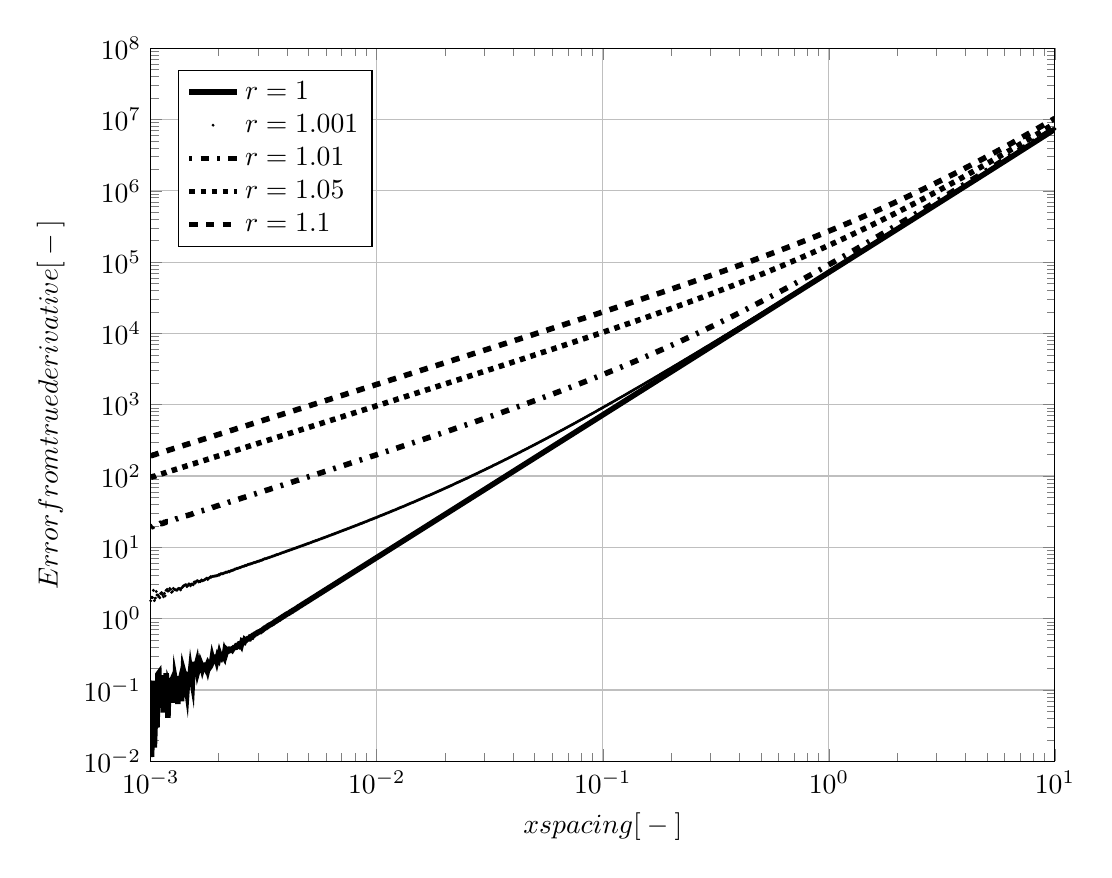
\begin{tikzpicture}

\begin{loglogaxis}[%
scale only axis,
width=4.52083in,
height=3.56562in,
xmin=0.001, xmax=10,
ymin=0.01, ymax=1e+08,
xminorticks=true,
yminorticks=true,
xlabel={$\text{x spacing [}-\text{]}$},
ylabel={$\text{Error from true derivative [}-\text{]}$},
xmajorgrids,
ymajorgrids,
legend entries={$\text{r }= 1$,$\text{r }= 1.001$,$\text{r }= 1.01$,$\text{r }= 1.05$,$\text{r }= 1.1$},
legend style={at={(0.03,0.97)},anchor=north west,nodes=right}]
\addplot [
color=black,
solid,
line width=2.0pt
]
coordinates{
 (0.001,0.0415039)(0.00100926,0.0115041)(0.00101861,0.0792145)(0.00102804,0.135215)(0.00103757,0.015545)(0.00104718,0.0369872)(0.00105688,0.122817)(0.00106666,0.0299618)(0.00107654,0.166037)(0.00108652,0.17287)(0.00109658,0.0576273)(0.00110674,0.119334)(0.00111699,0.113955)(0.00112733,0.143452)(0.00113777,0.0481481)(0.00114831,0.160899)(0.00115895,0.0714766)(0.00116968,0.17176)(0.00118052,0.118036)(0.00119145,0.0407878)(0.00120249,0.115287)(0.00121362,0.104929)(0.00122486,0.125567)(0.00123621,0.133927)(0.00124766,0.0797033)(0.00125922,0.0979223)(0.00127088,0.0663735)(0.00128265,0.138862)(0.00129453,0.117841)(0.00130652,0.12255)(0.00131862,0.063614)(0.00133083,0.155123)(0.00134316,0.126408)(0.0013556,0.142713)(0.00136816,0.0697708)(0.00138083,0.104354)(0.00139362,0.187977)(0.00140653,0.168443)(0.00141955,0.124795)(0.0014327,0.120643)(0.00144597,0.0974127)(0.00145937,0.149867)(0.00147288,0.144296)(0.00148652,0.137634)(0.00150029,0.183879)(0.00151419,0.150914)(0.00152821,0.126521)(0.00154237,0.228443)(0.00155665,0.228583)(0.00157107,0.207906)(0.00158562,0.213389)(0.00160031,0.238567)(0.00161513,0.186281)(0.00163009,0.207958)(0.00164519,0.208118)(0.00166043,0.239671)(0.00167581,0.222152)(0.00169133,0.198532)(0.00170699,0.220478)(0.00172281,0.222047)(0.00173876,0.216231)(0.00175487,0.202559)(0.00177112,0.217526)(0.00178753,0.194439)(0.00180408,0.219988)(0.00182079,0.206933)(0.00183766,0.215669)(0.00185468,0.231743)(0.00187186,0.281486)(0.00188919,0.250588)(0.00190669,0.256781)(0.00192435,0.288524)(0.00194217,0.287523)(0.00196016,0.257999)(0.00197832,0.292842)(0.00199664,0.27726)(0.00201514,0.320394)(0.0020338,0.293108)(0.00205264,0.282978)(0.00207165,0.302699)(0.00209084,0.306158)(0.0021102,0.290492)(0.00212975,0.349573)(0.00214947,0.326962)(0.00216938,0.359996)(0.00218948,0.348847)(0.00220976,0.352112)(0.00223022,0.372489)(0.00225088,0.370983)(0.00227173,0.374407)(0.00229277,0.364041)(0.00231401,0.381325)(0.00233544,0.392574)(0.00235707,0.394086)(0.0023789,0.396099)(0.00240093,0.420273)(0.00242317,0.421725)(0.00244562,0.414966)(0.00246827,0.444619)(0.00249113,0.447388)(0.0025142,0.425035)(0.00253749,0.475652)(0.00256099,0.465624)(0.00258471,0.463354)(0.00260865,0.505957)(0.00263282,0.494444)(0.0026572,0.508151)(0.00268181,0.521658)(0.00270665,0.520405)(0.00273172,0.520682)(0.00275702,0.555286)(0.00278256,0.561194)(0.00280833,0.555932)(0.00283434,0.583604)(0.0028606,0.589095)(0.00288709,0.605697)(0.00291383,0.613068)(0.00294082,0.620808)(0.00296806,0.639525)(0.00299555,0.648339)(0.00302329,0.655013)(0.0030513,0.65777)(0.00307956,0.67854)(0.00310808,0.686354)(0.00313687,0.704894)(0.00316592,0.721382)(0.00319525,0.73889)(0.00322484,0.745359)(0.00325471,0.763981)(0.00328486,0.775403)(0.00331528,0.796018)(0.00334599,0.810632)(0.00337698,0.821721)(0.00340826,0.833327)(0.00343983,0.849116)(0.00347169,0.861719)(0.00350384,0.88185)(0.0035363,0.901083)(0.00356905,0.916507)(0.00360211,0.93283)(0.00363547,0.951773)(0.00366914,0.970322)(0.00370313,0.983191)(0.00373743,1.00963)(0.00377204,1.02573)(0.00380698,1.04461)(0.00384224,1.06927)(0.00387783,1.08321)(0.00391375,1.108)(0.00395,1.1301)(0.00398658,1.14651)(0.00402351,1.17003)(0.00406077,1.1853)(0.00409838,1.20407)(0.00413634,1.23259)(0.00417466,1.25534)(0.00421332,1.27037)(0.00425235,1.30477)(0.00429173,1.32256)(0.00433148,1.34547)(0.0043716,1.36817)(0.00441209,1.39911)(0.00445296,1.42377)(0.0044942,1.45474)(0.00453583,1.48487)(0.00457784,1.50635)(0.00462024,1.5352)(0.00466303,1.56259)(0.00470622,1.59617)(0.00474981,1.62536)(0.00479381,1.65212)(0.00483821,1.6822)(0.00488302,1.72312)(0.00492825,1.745)(0.0049739,1.78167)(0.00501997,1.81344)(0.00506646,1.84292)(0.00511339,1.88317)(0.00516075,1.91697)(0.00520855,1.95778)(0.00525679,1.98555)(0.00530548,2.02688)(0.00535462,2.06273)(0.00540422,2.09912)(0.00545427,2.14182)(0.00550479,2.18614)(0.00555578,2.22374)(0.00560723,2.2641)(0.00565917,2.30486)(0.00571159,2.34917)(0.00576449,2.39163)(0.00581788,2.43787)(0.00587177,2.48258)(0.00592615,2.5301)(0.00598104,2.57419)(0.00603644,2.62196)(0.00609235,2.67258)(0.00614878,2.72445)(0.00620573,2.77213)(0.00626321,2.82293)(0.00632122,2.87875)(0.00637977,2.92728)(0.00643886,2.98341)(0.0064985,3.04508)(0.00655869,3.09327)(0.00661943,3.15549)(0.00668074,3.21154)(0.00674262,3.27306)(0.00680507,3.33192)(0.0068681,3.3971)(0.00693172,3.46004)(0.00699592,3.52417)(0.00706072,3.58837)(0.00712612,3.65608)(0.00719212,3.72255)(0.00725873,3.79441)(0.00732597,3.86536)(0.00739382,3.93554)(0.0074623,4.00837)(0.00753142,4.08239)(0.00760118,4.16172)(0.00767158,4.23594)(0.00774264,4.31642)(0.00781435,4.3963)(0.00788673,4.47844)(0.00795978,4.56359)(0.0080335,4.64664)(0.00810791,4.73202)(0.00818301,4.82292)(0.0082588,4.91031)(0.00833529,5.00361)(0.0084125,5.09714)(0.00849042,5.18963)(0.00856906,5.28569)(0.00864842,5.38396)(0.00872853,5.48424)(0.00880937,5.58732)(0.00889097,5.6896)(0.00897332,5.7976)(0.00905643,5.90537)(0.00914031,6.01491)(0.00922497,6.12648)(0.00931041,6.24174)(0.00939665,6.3569)(0.00948368,6.47642)(0.00957152,6.5948)(0.00966017,6.71805)(0.00974965,6.84253)(0.00983995,6.97058)(0.00993109,7.10142)(0.0100231,7.23325)(0.0101159,7.36747)(0.0102096,7.50438)(0.0103042,7.6451)(0.0103996,7.78667)(0.0104959,7.93205)(0.0105931,8.08002)(0.0106913,8.2299)(0.0107903,8.38323)(0.0108902,8.53967)(0.0109911,8.69799)(0.0110929,8.8611)(0.0111956,9.02412)(0.0112993,9.19212)(0.011404,9.3637)(0.0115096,9.53772)(0.0116162,9.71505)(0.0117238,9.89623)(0.0118324,10.0796)(0.011942,10.2683)(0.0120526,10.4588)(0.0121642,10.6534)(0.0122769,10.8523)(0.0123906,11.0539)(0.0125054,11.2596)(0.0126212,11.4693)(0.0127381,11.6823)(0.0128561,11.9003)(0.0129752,12.1217)(0.0130954,12.3464)(0.0132166,12.5766)(0.0133391,12.8113)(0.0134626,13.049)(0.0135873,13.2922)(0.0137131,13.5397)(0.0138402,13.7921)(0.0139684,14.0485)(0.0140977,14.3093)(0.0142283,14.5758)(0.0143601,14.8472)(0.0144931,15.1246)(0.0146273,15.4051)(0.0147628,15.6916)(0.0148996,15.984)(0.0150376,16.2814)(0.0151768,16.5842)(0.0153174,16.8931)(0.0154593,17.207)(0.0156025,17.5272)(0.015747,17.8538)(0.0158928,18.1858)(0.01604,18.5241)(0.0161886,18.8689)(0.0163385,19.2202)(0.0164899,19.5781)(0.0166426,19.9427)(0.0167967,20.3136)(0.0169523,20.6913)(0.0171093,21.0764)(0.0172678,21.4692)(0.0174277,21.8686)(0.0175892,22.2753)(0.0177521,22.6894)(0.0179165,23.112)(0.0180824,23.5421)(0.0182499,23.9801)(0.018419,24.4264)(0.0185896,24.8811)(0.0187617,25.3442)(0.0189355,25.816)(0.0191109,26.2964)(0.0192879,26.7861)(0.0194666,27.2842)(0.0196469,27.7918)(0.0198288,28.3091)(0.0200125,28.836)(0.0201979,29.3727)(0.0203849,29.9192)(0.0205737,30.4759)(0.0207643,31.0431)(0.0209566,31.6214)(0.0211507,32.2092)(0.0213466,32.8088)(0.0215443,33.4195)(0.0217439,34.0415)(0.0219453,34.6752)(0.0221486,35.32)(0.0223537,35.9775)(0.0225607,36.6468)(0.0227697,37.3292)(0.0229806,38.0236)(0.0231935,38.7314)(0.0234083,39.4521)(0.0236251,40.1864)(0.0238439,40.9343)(0.0240648,41.6959)(0.0242876,42.472)(0.0245126,43.2625)(0.0247396,44.0674)(0.0249688,44.8876)(0.0252,45.723)(0.0254335,46.5742)(0.025669,47.4407)(0.0259068,48.3235)(0.0261467,49.2229)(0.0263889,50.1389)(0.0266333,51.0719)(0.02688,52.0226)(0.027129,52.9906)(0.0273803,53.9769)(0.0276339,54.9813)(0.0278898,56.0045)(0.0281481,57.0468)(0.0284088,58.1087)(0.028672,59.19)(0.0289375,60.2914)(0.0292056,61.4133)(0.0294761,62.5563)(0.0297491,63.7205)(0.0300246,64.9064)(0.0303027,66.1143)(0.0305834,67.3447)(0.0308666,68.5981)(0.0311525,69.8746)(0.0314411,71.1751)(0.0317323,72.4996)(0.0320262,73.8488)(0.0323228,75.2232)(0.0326222,76.623)(0.0329244,78.0492)(0.0332293,79.5015)(0.0335371,80.981)(0.0338477,82.4882)(0.0341612,84.0232)(0.0344776,85.5869)(0.034797,87.1798)(0.0351193,88.8022)(0.0354446,90.4547)(0.0357729,92.1382)(0.0361042,93.853)(0.0364386,95.5995)(0.0367761,97.3787)(0.0371167,99.1908)(0.0374605,101.037)(0.0378075,102.917)(0.0381576,104.832)(0.0385111,106.783)(0.0388678,108.771)(0.0392278,110.795)(0.0395911,112.857)(0.0399578,114.957)(0.0403279,117.097)(0.0407014,119.276)(0.0410784,121.495)(0.0414589,123.757)(0.0418429,126.06)(0.0422304,128.406)(0.0426216,130.795)(0.0430164,133.229)(0.0434148,135.709)(0.0438169,138.234)(0.0442227,140.807)(0.0446323,143.427)(0.0450457,146.097)(0.045463,148.815)(0.045884,151.585)(0.046309,154.406)(0.046738,157.279)(0.0471708,160.206)(0.0476078,163.188)(0.0480487,166.225)(0.0484937,169.318)(0.0489429,172.469)(0.0493962,175.679)(0.0498537,178.949)(0.0503155,182.279)(0.0507815,185.671)(0.0512519,189.126)(0.0517266,192.646)(0.0522057,196.231)(0.0526892,199.883)(0.0531772,203.603)(0.0536698,207.392)(0.0541669,211.252)(0.0546686,215.183)(0.0551749,219.188)(0.055686,223.267)(0.0562017,227.422)(0.0567223,231.654)(0.0572477,235.965)(0.0577779,240.357)(0.0583131,244.83)(0.0588532,249.386)(0.0593983,254.027)(0.0599484,258.755)(0.0605037,263.57)(0.0610641,268.475)(0.0616297,273.472)(0.0622005,278.561)(0.0627766,283.745)(0.063358,289.026)(0.0639449,294.404)(0.0645372,299.883)(0.0651349,305.464)(0.0657382,311.149)(0.0663471,316.94)(0.0669616,322.838)(0.0675818,328.846)(0.0682078,334.966)(0.0688395,341.2)(0.0694771,347.549)(0.0701206,354.017)(0.0707701,360.606)(0.0714256,367.317)(0.0720872,374.152)(0.0727548,381.115)(0.0734287,388.208)(0.0741088,395.433)(0.0747952,402.792)(0.075488,410.288)(0.0761872,417.923)(0.0768928,425.701)(0.077605,433.623)(0.0783238,441.693)(0.0790493,449.913)(0.0797814,458.286)(0.0805204,466.815)(0.0812662,475.502)(0.0820189,484.352)(0.0827786,493.366)(0.0835453,502.547)(0.0843191,511.9)(0.0851001,521.426)(0.0858883,531.13)(0.0866838,541.014)(0.0874867,551.083)(0.088297,561.339)(0.0891148,571.785)(0.0899402,582.426)(0.0907733,593.265)(0.091614,604.306)(0.0924626,615.552)(0.093319,627.008)(0.0941833,638.677)(0.0950557,650.563)(0.0959361,662.67)(0.0968247,675.002)(0.0977215,687.564)(0.0986266,700.36)(0.0995401,713.394)(0.100462,726.67)(0.101393,740.193)(0.102332,753.969)(0.103279,768)(0.104236,782.293)(0.105202,796.851)(0.106176,811.681)(0.107159,826.787)(0.108152,842.173)(0.109154,857.846)(0.110165,873.811)(0.111185,890.073)(0.112215,906.637)(0.113254,923.51)(0.114303,940.697)(0.115362,958.203)(0.11643,976.035)(0.117509,994.2)(0.118597,1012.7)(0.119696,1031.55)(0.120804,1050.75)(0.121923,1070.3)(0.123052,1090.22)(0.124192,1110.51)(0.125342,1131.18)(0.126503,1152.23)(0.127675,1173.67)(0.128858,1195.51)(0.130051,1217.76)(0.131256,1240.42)(0.132471,1263.51)(0.133698,1287.02)(0.134937,1310.97)(0.136187,1335.37)(0.137448,1360.22)(0.138721,1385.54)(0.140006,1411.32)(0.141303,1437.59)(0.142611,1464.34)(0.143932,1491.59)(0.145265,1519.35)(0.146611,1547.63)(0.147969,1576.43)(0.149339,1605.77)(0.150723,1635.65)(0.152119,1666.09)(0.153528,1697.1)(0.15495,1728.68)(0.156385,1760.85)(0.157833,1793.62)(0.159295,1827)(0.16077,1861)(0.16226,1895.64)(0.163762,1930.91)(0.165279,1966.85)(0.16681,2003.45)(0.168355,2040.74)(0.169914,2078.72)(0.171488,2117.4)(0.173077,2156.81)(0.17468,2196.95)(0.176298,2237.83)(0.17793,2279.48)(0.179578,2321.9)(0.181242,2365.11)(0.18292,2409.13)(0.184615,2453.96)(0.186325,2499.63)(0.18805,2546.15)(0.189792,2593.53)(0.19155,2641.8)(0.193324,2690.96)(0.195115,2741.04)(0.196922,2792.05)(0.198746,2844.02)(0.200587,2896.94)(0.202445,2950.86)(0.20432,3005.77)(0.206212,3061.71)(0.208122,3118.69)(0.21005,3176.73)(0.211995,3235.85)(0.213959,3296.07)(0.215941,3357.41)(0.217941,3419.89)(0.219959,3483.54)(0.221997,3548.37)(0.224053,3614.41)(0.226128,3681.67)(0.228222,3750.19)(0.230336,3819.98)(0.23247,3891.07)(0.234623,3963.49)(0.236796,4037.25)(0.238989,4112.38)(0.241203,4188.91)(0.243437,4266.87)(0.245692,4346.28)(0.247967,4427.17)(0.250264,4509.56)(0.252582,4593.48)(0.254921,4678.97)(0.257283,4766.04)(0.259666,4854.74)(0.262071,4945.09)(0.264498,5037.12)(0.266948,5130.86)(0.26942,5226.35)(0.271916,5323.62)(0.274434,5422.69)(0.276976,5523.61)(0.279542,5626.41)(0.282131,5731.12)(0.284744,5837.77)(0.287381,5946.42)(0.290043,6057.08)(0.292729,6169.81)(0.295441,6284.63)(0.298177,6401.59)(0.300939,6520.73)(0.303726,6642.08)(0.30654,6765.69)(0.309379,6891.61)(0.312244,7019.86)(0.315136,7150.5)(0.318055,7283.58)(0.321001,7419.13)(0.323974,7557.2)(0.326975,7697.85)(0.330003,7841.11)(0.33306,7987.03)(0.336145,8135.68)(0.339258,8287.09)(0.342401,8441.31)(0.345572,8598.41)(0.348773,8758.43)(0.352003,8921.43)(0.355263,9087.46)(0.358554,9256.59)(0.361875,9428.86)(0.365227,9604.33)(0.36861,9783.08)(0.372024,9965.15)(0.375469,10150.6)(0.378947,10339.5)(0.382457,10531.9)(0.385999,10727.9)(0.389575,10927.6)(0.393183,11131)(0.396825,11338.1)(0.4005,11549.1)(0.40421,11764.1)(0.407953,11983)(0.411732,12206)(0.415546,12433.2)(0.419394,12664.6)(0.423279,12900.3)(0.427199,13140.4)(0.431156,13384.9)(0.43515,13634)(0.43918,13887.7)(0.443248,14146.2)(0.447353,14409.5)(0.451497,14677.7)(0.455679,14950.8)(0.459899,15229.1)(0.464159,15512.5)(0.468458,15801.2)(0.472797,16095.3)(0.477176,16394.8)(0.481596,16699.9)(0.486056,17010.7)(0.490558,17327.3)(0.495102,17649.8)(0.499688,17978.3)(0.504316,18312.9)(0.508987,18653.7)(0.513701,19000.8)(0.518459,19354.5)(0.523261,19714.7)(0.528108,20081.6)(0.532999,20455.3)(0.537936,20836)(0.542919,21223.8)(0.547947,21618.8)(0.553022,22021.2)(0.558145,22431)(0.563314,22848.5)(0.568532,23273.7)(0.573798,23706.8)(0.579112,24148.1)(0.584476,24597.5)(0.58989,25055.3)(0.595353,25521.6)(0.600868,25996.6)(0.606433,26480.4)(0.61205,26973.2)(0.617719,27475.3)(0.62344,27986.6)(0.629215,28507.5)(0.635043,29038)(0.640924,29578.5)(0.646861,30129)(0.652852,30689.7)(0.658899,31260.9)(0.665002,31842.7)(0.671161,32435.4)(0.677378,33039)(0.683652,33653.9)(0.689984,34280.3)(0.696374,34918.3)(0.702824,35568.2)(0.709334,36230.2)(0.715904,36904.5)(0.722535,37591.4)(0.729227,38291)(0.735981,39003.7)(0.742798,39729.6)(0.749678,40469)(0.756622,41222.2)(0.76363,41989.5)(0.770703,42771)(0.777841,43567)(0.785046,44377.9)(0.792317,45203.9)(0.799655,46045.2)(0.807062,46902.2)(0.814537,47775.2)(0.822082,48664.4)(0.829696,49570.1)(0.837381,50492.8)(0.845137,51432.5)(0.852964,52389.8)(0.860865,53364.9)(0.868838,54358.2)(0.876886,55369.9)(0.885007,56400.5)(0.893205,57450.3)(0.901478,58519.6)(0.909827,59608.8)(0.918254,60718.3)(0.926759,61848.4)(0.935343,62999.6)(0.944006,64172.2)(0.95275,65366.6)(0.961575,66583.3)(0.970481,67822.6)(0.97947,69085)(0.988542,70370.9)(0.997698,71680.7)(1.00694,73015)(1.01627,74374)(1.02568,75758.4)(1.03518,77168.5)(1.04477,78604.9)(1.05444,80068)(1.06421,81558.4)(1.07407,83076.5)(1.08401,84622.8)(1.09405,86198)(1.10419,87802.5)(1.11442,89436.8)(1.12474,91101.6)(1.13515,92797.4)(1.14567,94524.8)(1.15628,96284.3)(1.16699,98076.6)(1.1778,99902.2)(1.18871,101762)(1.19972,103656)(1.21083,105586)(1.22204,107551)(1.23336,109553)(1.24479,111592)(1.25632,113670)(1.26795,115786)(1.2797,117941)(1.29155,120137)(1.30351,122373)(1.31559,124651)(1.32777,126972)(1.34007,129335)(1.35248,131743)(1.36501,134195)(1.37765,136694)(1.39041,139238)(1.40329,141830)(1.41629,144471)(1.4294,147160)(1.44264,149900)(1.45601,152691)(1.46949,155533)(1.4831,158429)(1.49684,161378)(1.5107,164383)(1.5247,167443)(1.53882,170560)(1.55307,173736)(1.56746,176970)(1.58197,180265)(1.59663,183621)(1.61141,187040)(1.62634,190523)(1.6414,194070)(1.65661,197683)(1.67195,201364)(1.68744,205113)(1.70307,208932)(1.71884,212822)(1.73476,216785)(1.75083,220821)(1.76704,224933)(1.78341,229121)(1.79993,233387)(1.8166,237733)(1.83343,242160)(1.85041,246669)(1.86755,251262)(1.88484,255941)(1.9023,260707)(1.91992,265562)(1.9377,270507)(1.95565,275545)(1.97376,280676)(1.99205,285903)(2.0105,291227)(2.02912,296650)(2.04791,302175)(2.06688,307803)(2.08602,313535)(2.10535,319374)(2.12485,325322)(2.14453,331381)(2.16439,337553)(2.18444,343840)(2.20467,350244)(2.22509,356768)(2.2457,363413)(2.2665,370182)(2.28749,377077)(2.30868,384100)(2.33006,391255)(2.35164,398543)(2.37342,405967)(2.39541,413529)(2.41759,421233)(2.43999,429080)(2.46259,437073)(2.48539,445215)(2.50842,453510)(2.53165,461959)(2.5551,470565)(2.57876,479332)(2.60265,488262)(2.62675,497360)(2.65108,506626)(2.67564,516066)(2.70042,525682)(2.72543,535477)(2.75068,545455)(2.77615,555619)(2.80187,565972)(2.82782,576519)(2.85401,587263)(2.88044,598207)(2.90712,609355)(2.93405,620712)(2.96123,632280)(2.98865,644065)(3.01633,656069)(3.04427,668297)(3.07247,680754)(3.10093,693443)(3.12965,706369)(3.15864,719537)(3.18789,732950)(3.21742,746614)(3.24722,760533)(3.27729,774712)(3.30765,789156)(3.33829,803869)(3.36921,818858)(3.40041,834126)(3.43191,849680)(3.46369,865524)(3.49578,881664)(3.52815,898106)(3.56083,914855)(3.59381,931917)(3.6271,949299)(3.6607,967005)(3.6946,985042)(3.72882,1.00342e+06)(3.76336,1.02213e+06)(3.79822,1.0412e+06)(3.8334,1.06063e+06)(3.8689,1.08041e+06)(3.90474,1.10057e+06)(3.9409,1.12111e+06)(3.9774,1.14202e+06)(4.01424,1.16333e+06)(4.05142,1.18504e+06)(4.08895,1.20716e+06)(4.12682,1.22969e+06)(4.16504,1.25264e+06)(4.20362,1.27602e+06)(4.24256,1.29984e+06)(4.28185,1.3241e+06)(4.32151,1.34882e+06)(4.36154,1.374e+06)(4.40194,1.39965e+06)(4.44271,1.42579e+06)(4.48386,1.45241e+06)(4.52539,1.47953e+06)(4.5673,1.50716e+06)(4.6096,1.53531e+06)(4.6523,1.56398e+06)(4.69539,1.59319e+06)(4.73888,1.62295e+06)(4.78277,1.65327e+06)(4.82707,1.68416e+06)(4.87178,1.71563e+06)(4.9169,1.74768e+06)(4.96244,1.78034e+06)(5.00841,1.81361e+06)(5.0548,1.8475e+06)(5.10162,1.88204e+06)(5.14887,1.91721e+06)(5.19656,1.95305e+06)(5.24469,1.98957e+06)(5.29327,2.02676e+06)(5.34229,2.06466e+06)(5.39177,2.10327e+06)(5.44171,2.1426e+06)(5.49212,2.18268e+06)(5.54299,2.22351e+06)(5.59433,2.2651e+06)(5.64614,2.30748e+06)(5.69844,2.35065e+06)(5.75122,2.39464e+06)(5.80449,2.43945e+06)(5.85825,2.48511e+06)(5.91251,2.53162e+06)(5.96727,2.57901e+06)(6.02254,2.6273e+06)(6.07832,2.67649e+06)(6.13462,2.72661e+06)(6.19144,2.77768e+06)(6.24879,2.82971e+06)(6.30667,2.88271e+06)(6.36508,2.93672e+06)(6.42403,2.99175e+06)(6.48353,3.04781e+06)(6.54359,3.10493e+06)(6.60419,3.16313e+06)(6.66536,3.22243e+06)(6.7271,3.28285e+06)(6.78941,3.34441e+06)(6.85229,3.40714e+06)(6.91576,3.47105e+06)(6.97981,3.53616e+06)(7.04446,3.60251e+06)(7.10971,3.67011e+06)(7.17556,3.739e+06)(7.24202,3.80918e+06)(7.3091,3.8807e+06)(7.3768,3.95357e+06)(7.44512,4.02782e+06)(7.51408,4.10348e+06)(7.58368,4.18057e+06)(7.65392,4.25912e+06)(7.72481,4.33917e+06)(7.79636,4.42073e+06)(7.86857,4.50384e+06)(7.94145,4.58853e+06)(8.01501,4.67483e+06)(8.08924,4.76276e+06)(8.16417,4.85237e+06)(8.23979,4.94369e+06)(8.3161,5.03674e+06)(8.39313,5.13156e+06)(8.47087,5.22819e+06)(8.54933,5.32666e+06)(8.62851,5.427e+06)(8.70843,5.52926e+06)(8.78909,5.63347e+06)(8.8705,5.73967e+06)(8.95266,5.84789e+06)(9.03558,5.95819e+06)(9.11927,6.07058e+06)(9.20373,6.18513e+06)(9.28898,6.30187e+06)(9.37502,6.42084e+06)(9.46185,6.54209e+06)(9.54949,6.66567e+06)(9.63793,6.79161e+06)(9.7272,6.91996e+06)(9.8173,7.05078e+06)(9.90823,7.18411e+06)(10,7.32e+06) 
};

\addplot [
color=black,
mark size=0.3pt,
only marks,
mark=*,
mark options={solid}
]
coordinates{
 (0.001,1.77815)(0.00100926,1.99566)(0.00101861,1.97797)(0.00102804,2.49542)(0.00103757,1.79286)(0.00104718,1.93642)(0.00105688,2.40386)(0.00106666,2.14426)(0.00107654,2.15083)(0.00108652,2.05346)(0.00109658,1.95879)(0.00110674,2.2614)(0.00111699,2.31788)(0.00112733,2.16976)(0.00113777,2.02822)(0.00114831,2.26438)(0.00115895,2.08396)(0.00116968,2.49925)(0.00118052,2.57599)(0.00119145,2.43847)(0.00120249,2.45891)(0.00121362,2.64085)(0.00122486,2.58415)(0.00123621,2.3405)(0.00124766,2.39118)(0.00125922,2.65646)(0.00127088,2.56711)(0.00128265,2.55943)(0.00129453,2.51973)(0.00130652,2.5077)(0.00131862,2.60788)(0.00133083,2.65158)(0.00134316,2.63531)(0.0013556,2.53146)(0.00136816,2.68881)(0.00138083,2.75315)(0.00139362,2.87922)(0.00140653,2.90342)(0.00141955,2.97953)(0.0014327,2.98757)(0.00144597,2.81863)(0.00145937,2.89504)(0.00147288,3.0674)(0.00148652,3.04894)(0.00150029,2.88769)(0.00151419,3.05018)(0.00152821,3.04312)(0.00154237,2.9977)(0.00155665,3.26718)(0.00157107,3.15274)(0.00158562,3.29648)(0.00160031,3.38854)(0.00161513,3.39816)(0.00163009,3.27855)(0.00164519,3.3181)(0.00166043,3.31479)(0.00167581,3.48854)(0.00169133,3.39606)(0.00170699,3.44236)(0.00172281,3.47703)(0.00173876,3.53676)(0.00175487,3.60907)(0.00177112,3.70149)(0.00178753,3.53168)(0.00180408,3.68854)(0.00182079,3.73108)(0.00183766,3.87658)(0.00185468,3.83408)(0.00187186,3.91742)(0.00188919,3.91797)(0.00190669,3.94233)(0.00192435,3.96819)(0.00194217,3.97394)(0.00196016,3.99901)(0.00197832,4.03127)(0.00199664,4.12976)(0.00201514,4.10162)(0.0020338,4.24666)(0.00205264,4.2631)(0.00207165,4.27425)(0.00209084,4.28222)(0.0021102,4.35938)(0.00212975,4.3855)(0.00214947,4.49452)(0.00216938,4.48467)(0.00218948,4.50059)(0.00220976,4.6016)(0.00223022,4.55849)(0.00225088,4.67791)(0.00227173,4.68849)(0.00229277,4.77637)(0.00231401,4.77159)(0.00233544,4.86775)(0.00235707,4.96943)(0.0023789,4.95989)(0.00240093,5.05598)(0.00242317,5.08613)(0.00244562,5.11723)(0.00246827,5.18251)(0.00249113,5.21987)(0.0025142,5.28062)(0.00253749,5.36619)(0.00256099,5.41657)(0.00258471,5.4293)(0.00260865,5.53681)(0.00263282,5.55814)(0.0026572,5.59676)(0.00268181,5.69597)(0.00270665,5.77206)(0.00273172,5.80805)(0.00275702,5.84886)(0.00278256,5.90886)(0.00280833,5.96053)(0.00283434,6.02598)(0.0028606,6.09282)(0.00288709,6.15084)(0.00291383,6.17958)(0.00294082,6.27139)(0.00296806,6.34695)(0.00299555,6.39535)(0.00302329,6.42376)(0.0030513,6.52973)(0.00307956,6.59304)(0.00310808,6.62722)(0.00313687,6.74249)(0.00316592,6.81184)(0.00319525,6.90476)(0.00322484,6.93123)(0.00325471,6.99384)(0.00328486,7.10323)(0.00331528,7.14816)(0.00334599,7.23649)(0.00337698,7.29498)(0.00340826,7.37542)(0.00343983,7.46087)(0.00347169,7.55477)(0.00350384,7.59106)(0.0035363,7.7029)(0.00356905,7.78016)(0.00360211,7.85532)(0.00363547,7.92324)(0.00366914,7.99497)(0.00370313,8.09928)(0.00373743,8.19017)(0.00377204,8.26161)(0.00380698,8.36392)(0.00384224,8.46037)(0.00387783,8.54726)(0.00391375,8.61157)(0.00395,8.72994)(0.00398658,8.81014)(0.00402351,8.90398)(0.00406077,9.00733)(0.00409838,9.09425)(0.00413634,9.1788)(0.00417466,9.26754)(0.00421332,9.37245)(0.00425235,9.47652)(0.00429173,9.56516)(0.00433148,9.67709)(0.0043716,9.76393)(0.00441209,9.88243)(0.00445296,9.97886)(0.0044942,10.0924)(0.00453583,10.1844)(0.00457784,10.2963)(0.00462024,10.4157)(0.00466303,10.5293)(0.00470622,10.6367)(0.00474981,10.7488)(0.00479381,10.853)(0.00483821,10.9755)(0.00488302,11.0934)(0.00492825,11.2128)(0.0049739,11.3341)(0.00501997,11.4572)(0.00506646,11.5645)(0.00511339,11.694)(0.00516075,11.8288)(0.00520855,11.9591)(0.00525679,12.0832)(0.00530548,12.2277)(0.00535462,12.3509)(0.00540422,12.482)(0.00545427,12.6209)(0.00550479,12.7518)(0.00555578,12.8938)(0.00560723,13.034)(0.00565917,13.171)(0.00571159,13.309)(0.00576449,13.4685)(0.00581788,13.6066)(0.00587177,13.7544)(0.00592615,13.9162)(0.00598104,14.0565)(0.00603644,14.2185)(0.00609235,14.3773)(0.00614878,14.53)(0.00620573,14.6875)(0.00626321,14.8442)(0.00632122,15.0225)(0.00637977,15.1818)(0.00643886,15.3473)(0.0064985,15.5164)(0.00655869,15.6962)(0.00661943,15.8714)(0.00668074,16.0452)(0.00674262,16.226)(0.00680507,16.4011)(0.0068681,16.5906)(0.00693172,16.7747)(0.00699592,16.9521)(0.00706072,17.1562)(0.00712612,17.3443)(0.00719212,17.5349)(0.00725873,17.7307)(0.00732597,17.9351)(0.00739382,18.1317)(0.0074623,18.3476)(0.00753142,18.5485)(0.00760118,18.7559)(0.00767158,18.97)(0.00774264,19.1818)(0.00781435,19.4028)(0.00788673,19.6284)(0.00795978,19.847)(0.0080335,20.0768)(0.00810791,20.3042)(0.00818301,20.5398)(0.0082588,20.7774)(0.00833529,21.0122)(0.0084125,21.2521)(0.00849042,21.498)(0.00856906,21.7458)(0.00864842,21.998)(0.00872853,22.2484)(0.00880937,22.5084)(0.00889097,22.7673)(0.00897332,23.0315)(0.00905643,23.2982)(0.00914031,23.5707)(0.00922497,23.8469)(0.00931041,24.1257)(0.00939665,24.4073)(0.00948368,24.6939)(0.00957152,24.9839)(0.00966017,25.2697)(0.00974965,25.5703)(0.00983995,25.8695)(0.00993109,26.177)(0.0100231,26.4864)(0.0101159,26.7987)(0.0102096,27.1132)(0.0103042,27.4333)(0.0103996,27.7654)(0.0104959,28.0943)(0.0105931,28.4279)(0.0106913,28.7637)(0.0107903,29.1104)(0.0108902,29.4554)(0.0109911,29.8102)(0.0110929,30.1683)(0.0111956,30.5307)(0.0112993,30.8968)(0.011404,31.2692)(0.0115096,31.6428)(0.0116162,32.0295)(0.0117238,32.4175)(0.0118324,32.8105)(0.011942,33.2076)(0.0120526,33.61)(0.0121642,34.02)(0.0122769,34.4335)(0.0123906,34.8527)(0.0125054,35.2838)(0.0126212,35.7138)(0.0127381,36.1509)(0.0128561,36.5938)(0.0129752,37.0463)(0.0130954,37.503)(0.0132166,37.9653)(0.0133391,38.4341)(0.0134626,38.9106)(0.0135873,39.3928)(0.0137131,39.8819)(0.0138402,40.378)(0.0139684,40.8813)(0.0140977,41.3912)(0.0142283,41.9088)(0.0143601,42.4336)(0.0144931,42.9652)(0.0146273,43.506)(0.0147628,44.0513)(0.0148996,44.6063)(0.0150376,45.1688)(0.0151768,45.7392)(0.0153174,46.3208)(0.0154593,46.9066)(0.0156025,47.5007)(0.015747,48.1051)(0.0158928,48.7187)(0.01604,49.3399)(0.0161886,49.9701)(0.0163385,50.6109)(0.0164899,51.2586)(0.0166426,51.9176)(0.0167967,52.5833)(0.0169523,53.2616)(0.0171093,53.9477)(0.0172678,54.645)(0.0174277,55.3512)(0.0175892,56.069)(0.0177521,56.7958)(0.0179165,57.5356)(0.0180824,58.285)(0.0182499,59.045)(0.018419,59.8165)(0.0185896,60.5979)(0.0187617,61.3929)(0.0189355,62.1979)(0.0191109,63.0155)(0.0192879,63.8456)(0.0194666,64.6875)(0.0196469,65.5421)(0.0198288,66.4087)(0.0200125,67.2895)(0.0201979,68.1823)(0.0203849,69.0886)(0.0205737,70.0088)(0.0207643,70.9419)(0.0209566,71.8891)(0.0211507,72.8509)(0.0213466,73.8277)(0.0215443,74.8184)(0.0217439,75.824)(0.0219453,76.8457)(0.0221486,77.8807)(0.0223537,78.9327)(0.0225607,80.0003)(0.0227697,81.0844)(0.0229806,82.1847)(0.0231935,83.3023)(0.0234083,84.4355)(0.0236251,85.587)(0.0238439,86.7562)(0.0240648,87.9422)(0.0242876,89.1474)(0.0245126,90.3705)(0.0247396,91.6121)(0.0249688,92.873)(0.0252,94.153)(0.0254335,95.4529)(0.025669,96.7733)(0.0259068,98.1137)(0.0261467,99.474)(0.0263889,100.856)(0.0266333,102.259)(0.02688,103.685)(0.027129,105.132)(0.0273803,106.601)(0.0276339,108.093)(0.0278898,109.609)(0.0281481,111.149)(0.0284088,112.712)(0.028672,114.3)(0.0289375,115.912)(0.0292056,117.55)(0.0294761,119.213)(0.0297491,120.903)(0.0300246,122.619)(0.0303027,124.362)(0.0305834,126.133)(0.0308666,127.931)(0.0311525,129.758)(0.0314411,131.613)(0.0317323,133.498)(0.0320262,135.413)(0.0323228,137.359)(0.0326222,139.335)(0.0329244,141.342)(0.0332293,143.382)(0.0335371,145.453)(0.0338477,147.559)(0.0341612,149.697)(0.0344776,151.87)(0.034797,154.078)(0.0351193,156.321)(0.0354446,158.599)(0.0357729,160.915)(0.0361042,163.267)(0.0364386,165.657)(0.0367761,168.087)(0.0371167,170.555)(0.0374605,173.062)(0.0378075,175.611)(0.0381576,178.2)(0.0385111,180.832)(0.0388678,183.506)(0.0392278,186.223)(0.0395911,188.985)(0.0399578,191.792)(0.0403279,194.644)(0.0407014,197.542)(0.0410784,200.488)(0.0414589,203.482)(0.0418429,206.525)(0.0422304,209.617)(0.0426216,212.76)(0.0430164,215.955)(0.0434148,219.201)(0.0438169,222.502)(0.0442227,225.856)(0.0446323,229.266)(0.0450457,232.731)(0.045463,236.254)(0.045884,239.835)(0.046309,243.474)(0.046738,247.174)(0.0471708,250.936)(0.0476078,254.759)(0.0480487,258.646)(0.0484937,262.597)(0.0489429,266.613)(0.0493962,270.696)(0.0498537,274.848)(0.0503155,279.068)(0.0507815,283.358)(0.0512519,287.72)(0.0517266,292.155)(0.0522057,296.664)(0.0526892,301.247)(0.0531772,305.908)(0.0536698,310.647)(0.0541669,315.464)(0.0546686,320.363)(0.0551749,325.344)(0.055686,330.408)(0.0562017,335.558)(0.0567223,340.794)(0.0572477,346.118)(0.0577779,351.532)(0.0583131,357.037)(0.0588532,362.635)(0.0593983,368.327)(0.0599484,374.116)(0.0605037,380.002)(0.0610641,385.988)(0.0616297,392.076)(0.0622005,398.266)(0.0627766,404.561)(0.063358,410.964)(0.0639449,417.475)(0.0645372,424.096)(0.0651349,430.83)(0.0657382,437.679)(0.0663471,444.645)(0.0669616,451.729)(0.0675818,458.934)(0.0682078,466.261)(0.0688395,473.715)(0.0694771,481.295)(0.0701206,489.005)(0.0707701,496.847)(0.0714256,504.823)(0.0720872,512.936)(0.0727548,521.188)(0.0734287,529.582)(0.0741088,538.119)(0.0747952,546.804)(0.075488,555.637)(0.0761872,564.623)(0.0768928,573.763)(0.077605,583.061)(0.0783238,592.519)(0.0790493,602.14)(0.0797814,611.927)(0.0805204,621.884)(0.0812662,632.012)(0.0820189,642.315)(0.0827786,652.797)(0.0835453,663.46)(0.0843191,674.307)(0.0851001,685.343)(0.0858883,696.57)(0.0866838,707.992)(0.0874867,719.612)(0.088297,731.433)(0.0891148,743.461)(0.0899402,755.697)(0.0907733,768.147)(0.091614,780.813)(0.0924626,793.7)(0.093319,806.811)(0.0941833,820.151)(0.0950557,833.724)(0.0959361,847.534)(0.0968247,861.585)(0.0977215,875.881)(0.0986266,890.427)(0.0995401,905.228)(0.100462,920.288)(0.101393,935.612)(0.102332,951.204)(0.103279,967.069)(0.104236,983.213)(0.105202,999.64)(0.106176,1016.36)(0.107159,1033.36)(0.108152,1050.67)(0.109154,1068.28)(0.110165,1086.21)(0.111185,1104.44)(0.112215,1123)(0.113254,1141.89)(0.114303,1161.11)(0.115362,1180.66)(0.11643,1200.56)(0.117509,1220.82)(0.118597,1241.43)(0.119696,1262.4)(0.120804,1283.75)(0.121923,1305.47)(0.123052,1327.58)(0.124192,1350.08)(0.125342,1372.97)(0.126503,1396.27)(0.127675,1419.99)(0.128858,1444.12)(0.130051,1468.69)(0.131256,1493.68)(0.132471,1519.13)(0.133698,1545.02)(0.134937,1571.37)(0.136187,1598.19)(0.137448,1625.49)(0.138721,1653.28)(0.140006,1681.56)(0.141303,1710.34)(0.142611,1739.63)(0.143932,1769.45)(0.145265,1799.79)(0.146611,1830.68)(0.147969,1862.12)(0.149339,1894.12)(0.150723,1926.69)(0.152119,1959.84)(0.153528,1993.58)(0.15495,2027.93)(0.156385,2062.88)(0.157833,2098.47)(0.159295,2134.69)(0.16077,2171.56)(0.16226,2209.08)(0.163762,2247.28)(0.165279,2286.17)(0.16681,2325.75)(0.168355,2366.04)(0.169914,2407.05)(0.171488,2448.79)(0.173077,2491.29)(0.17468,2534.55)(0.176298,2578.58)(0.17793,2623.4)(0.179578,2669.03)(0.181242,2715.48)(0.18292,2762.76)(0.184615,2810.9)(0.186325,2859.89)(0.18805,2909.77)(0.189792,2960.55)(0.19155,3012.24)(0.193324,3064.86)(0.195115,3118.43)(0.196922,3172.96)(0.198746,3228.48)(0.200587,3284.99)(0.202445,3342.53)(0.20432,3401.1)(0.206212,3460.73)(0.208122,3521.43)(0.21005,3583.23)(0.211995,3646.15)(0.213959,3710.2)(0.215941,3775.41)(0.217941,3841.79)(0.219959,3909.38)(0.221997,3978.19)(0.224053,4048.24)(0.226128,4119.56)(0.228222,4192.16)(0.230336,4266.09)(0.23247,4341.35)(0.234623,4417.97)(0.236796,4495.98)(0.238989,4575.4)(0.241203,4656.26)(0.243437,4738.58)(0.245692,4822.4)(0.247967,4907.74)(0.250264,4994.62)(0.252582,5083.08)(0.254921,5173.15)(0.257283,5264.85)(0.259666,5358.21)(0.262071,5453.27)(0.264498,5550.06)(0.266948,5648.6)(0.26942,5748.93)(0.271916,5851.08)(0.274434,5955.09)(0.276976,6061)(0.279542,6168.82)(0.282131,6278.61)(0.284744,6390.39)(0.287381,6504.21)(0.290043,6620.1)(0.292729,6738.1)(0.295441,6858.24)(0.298177,6980.58)(0.300939,7105.14)(0.303726,7231.97)(0.30654,7361.11)(0.309379,7492.6)(0.312244,7626.49)(0.315136,7762.82)(0.318055,7901.63)(0.321001,8042.98)(0.323974,8186.9)(0.326975,8333.45)(0.330003,8482.67)(0.33306,8634.61)(0.336145,8789.33)(0.339258,8946.87)(0.342401,9107.29)(0.345572,9270.64)(0.348773,9436.97)(0.352003,9606.34)(0.355263,9778.8)(0.358554,9954.41)(0.361875,10133.2)(0.365227,10315.3)(0.36861,10500.7)(0.372024,10689.6)(0.375469,10881.8)(0.378947,11077.6)(0.382457,11277)(0.385999,11480)(0.389575,11686.7)(0.393183,11897.2)(0.396825,12111.6)(0.4005,12329.8)(0.40421,12552.1)(0.407953,12778.5)(0.411732,13009)(0.415546,13243.7)(0.419394,13482.7)(0.423279,13726.1)(0.427199,13974)(0.431156,14226.4)(0.43515,14483.4)(0.43918,14745.1)(0.443248,15011.7)(0.447353,15283.1)(0.451497,15559.5)(0.455679,15841)(0.459899,16127.6)(0.464159,16419.5)(0.468458,16716.7)(0.472797,17019.5)(0.477176,17327.7)(0.481596,17641.6)(0.486056,17961.3)(0.490558,18286.9)(0.495102,18618.4)(0.499688,18956)(0.504316,19299.9)(0.508987,19650)(0.513701,20006.6)(0.518459,20369.7)(0.523261,20739.5)(0.528108,21116.1)(0.532999,21499.6)(0.537936,21890.2)(0.542919,22287.9)(0.547947,22693)(0.553022,23105.5)(0.558145,23525.6)(0.563314,23953.4)(0.568532,24389.1)(0.573798,24832.8)(0.579112,25284.7)(0.584476,25744.9)(0.58989,26213.5)(0.595353,26690.8)(0.600868,27176.9)(0.606433,27671.9)(0.61205,28176)(0.617719,28689.5)(0.62344,29212.3)(0.629215,29744.8)(0.635043,30287.1)(0.640924,30839.4)(0.646861,31401.9)(0.652852,31974.7)(0.658899,32558.1)(0.665002,33152.3)(0.671161,33757.3)(0.677378,34373.6)(0.683652,35001.2)(0.689984,35640.3)(0.696374,36291.3)(0.702824,36954.2)(0.709334,37629.4)(0.715904,38317)(0.722535,39017.3)(0.729227,39730.6)(0.735981,40457)(0.742798,41196.7)(0.749678,41950.2)(0.756622,42717.5)(0.76363,43499)(0.770703,44294.9)(0.777841,45105.5)(0.785046,45931)(0.792317,46771.8)(0.799655,47628.1)(0.807062,48500.3)(0.814537,49388.5)(0.822082,50293.1)(0.829696,51214.4)(0.837381,52152.8)(0.845137,53108.4)(0.852964,54081.8)(0.860865,55073.1)(0.868838,56082.7)(0.876886,57110.9)(0.885007,58158.2)(0.893205,59224.8)(0.901478,60311.1)(0.909827,61417.5)(0.918254,62544.4)(0.926759,63692)(0.935343,64860.9)(0.944006,66051.4)(0.95275,67263.9)(0.961575,68498.8)(0.970481,69756.5)(0.97947,71037.5)(0.988542,72342.2)(0.997698,73671)(1.00694,75024.3)(1.01627,76402.7)(1.02568,77806.6)(1.03518,79236.5)(1.04477,80692.8)(1.05444,82176.1)(1.06421,83686.8)(1.07407,85225.4)(1.08401,86792.6)(1.09405,88388.7)(1.10419,90014.3)(1.11442,91670.1)(1.12474,93356.4)(1.13515,95074)(1.14567,96823.4)(1.15628,98605.2)(1.16699,100420)(1.1778,102268)(1.18871,104151)(1.19972,106068)(1.21083,108021)(1.22204,110010)(1.23336,112036)(1.24479,114100)(1.25632,116201)(1.26795,118342)(1.2797,120522)(1.29155,122743)(1.30351,125005)(1.31559,127308)(1.32777,129655)(1.34007,132045)(1.35248,134479)(1.36501,136958)(1.37765,139483)(1.39041,142055)(1.40329,144675)(1.41629,147343)(1.4294,150061)(1.44264,152829)(1.45601,155648)(1.46949,158520)(1.4831,161444)(1.49684,164423)(1.5107,167458)(1.5247,170548)(1.53882,173696)(1.55307,176903)(1.56746,180168)(1.58197,183495)(1.59663,186883)(1.61141,190333)(1.62634,193848)(1.6414,197428)(1.65661,201075)(1.67195,204789)(1.68744,208572)(1.70307,212425)(1.71884,216350)(1.73476,220348)(1.75083,224419)(1.76704,228567)(1.78341,232791)(1.79993,237094)(1.8166,241476)(1.83343,245940)(1.85041,250487)(1.86755,255118)(1.88484,259836)(1.9023,264641)(1.91992,269535)(1.9377,274519)(1.95565,279597)(1.97376,284769)(1.99205,290037)(2.0105,295402)(2.02912,300868)(2.04791,306434)(2.06688,312105)(2.08602,317880)(2.10535,323763)(2.12485,329756)(2.14453,335859)(2.16439,342076)(2.18444,348409)(2.20467,354859)(2.22509,361429)(2.2457,368121)(2.2665,374938)(2.28749,381881)(2.30868,388953)(2.33006,396157)(2.35164,403495)(2.37342,410969)(2.39541,418583)(2.41759,426337)(2.43999,434236)(2.46259,442282)(2.48539,450478)(2.50842,458826)(2.53165,467329)(2.5551,475990)(2.57876,484813)(2.60265,493800)(2.62675,502954)(2.65108,512278)(2.67564,521776)(2.70042,531450)(2.72543,541305)(2.75068,551343)(2.77615,561568)(2.80187,571983)(2.82782,582592)(2.85401,593398)(2.88044,604406)(2.90712,615619)(2.93405,627040)(2.96123,638675)(2.98865,650526)(3.01633,662597)(3.04427,674894)(3.07247,687419)(3.10093,700178)(3.12965,713175)(3.15864,726414)(3.18789,739899)(3.21742,753636)(3.24722,767629)(3.27729,781883)(3.30765,796402)(3.33829,811192)(3.36921,826258)(3.40041,841605)(3.43191,857238)(3.46369,873162)(3.49578,889384)(3.52815,905908)(3.56083,922740)(3.59381,939886)(3.6271,957353)(3.6607,975145)(3.6946,993269)(3.72882,1.01173e+06)(3.76336,1.03054e+06)(3.79822,1.0497e+06)(3.8334,1.06921e+06)(3.8689,1.08909e+06)(3.90474,1.10934e+06)(3.9409,1.12997e+06)(3.9774,1.15099e+06)(4.01424,1.1724e+06)(4.05142,1.1942e+06)(4.08895,1.21642e+06)(4.12682,1.23905e+06)(4.16504,1.2621e+06)(4.20362,1.28558e+06)(4.24256,1.30951e+06)(4.28185,1.33388e+06)(4.32151,1.3587e+06)(4.36154,1.38399e+06)(4.40194,1.40976e+06)(4.44271,1.436e+06)(4.48386,1.46274e+06)(4.52539,1.48997e+06)(4.5673,1.51772e+06)(4.6096,1.54598e+06)(4.6523,1.57478e+06)(4.69539,1.60411e+06)(4.73888,1.63399e+06)(4.78277,1.66443e+06)(4.82707,1.69544e+06)(4.87178,1.72704e+06)(4.9169,1.75922e+06)(4.96244,1.79201e+06)(5.00841,1.82541e+06)(5.0548,1.85944e+06)(5.10162,1.8941e+06)(5.14887,1.92942e+06)(5.19656,1.9654e+06)(5.24469,2.00205e+06)(5.29327,2.03939e+06)(5.34229,2.07743e+06)(5.39177,2.11619e+06)(5.44171,2.15567e+06)(5.49212,2.1959e+06)(5.54299,2.23688e+06)(5.59433,2.27863e+06)(5.64614,2.32116e+06)(5.69844,2.36449e+06)(5.75122,2.40864e+06)(5.80449,2.45361e+06)(5.85825,2.49944e+06)(5.91251,2.54612e+06)(5.96727,2.59368e+06)(6.02254,2.64214e+06)(6.07832,2.69151e+06)(6.13462,2.7418e+06)(6.19144,2.79305e+06)(6.24879,2.84526e+06)(6.30667,2.89845e+06)(6.36508,2.95265e+06)(6.42403,3.00786e+06)(6.48353,3.06412e+06)(6.54359,3.12144e+06)(6.60419,3.17983e+06)(6.66536,3.23933e+06)(6.7271,3.29996e+06)(6.78941,3.36172e+06)(6.85229,3.42466e+06)(6.91576,3.48878e+06)(6.97981,3.55411e+06)(7.04446,3.62068e+06)(7.10971,3.68851e+06)(7.17556,3.75761e+06)(7.24202,3.82803e+06)(7.3091,3.89978e+06)(7.3768,3.97288e+06)(7.44512,4.04737e+06)(7.51408,4.12327e+06)(7.58368,4.20061e+06)(7.65392,4.27941e+06)(7.72481,4.35971e+06)(7.79636,4.44153e+06)(7.86857,4.52491e+06)(7.94145,4.60986e+06)(8.01501,4.69643e+06)(8.08924,4.78464e+06)(8.16417,4.87453e+06)(8.23979,4.96613e+06)(8.3161,5.05946e+06)(8.39313,5.15458e+06)(8.47087,5.2515e+06)(8.54933,5.35027e+06)(8.62851,5.45092e+06)(8.70843,5.55349e+06)(8.78909,5.65801e+06)(8.8705,5.76453e+06)(8.95266,5.87308e+06)(9.03558,5.9837e+06)(9.11927,6.09644e+06)(9.20373,6.21133e+06)(9.28898,6.32841e+06)(9.37502,6.44774e+06)(9.46185,6.56935e+06)(9.54949,6.69328e+06)(9.63793,6.81959e+06)(9.7272,6.94833e+06)(9.8173,7.07953e+06)(9.90823,7.21325e+06)(10,7.34953e+06) 
};

\addplot [
color=black,
dash pattern=on 1pt off 3pt on 3pt off 3pt,
line width=2.0pt
]
coordinates{
 (0.001,19.1522)(0.00100926,19.4287)(0.00101861,19.578)(0.00102804,20.2053)(0.00103757,19.7577)(0.00104718,19.9567)(0.00105688,20.5326)(0.00106666,20.6797)(0.00107654,20.7149)(0.00108652,21.0745)(0.00109658,21.144)(0.00110674,21.6636)(0.00111699,21.5108)(0.00112733,21.6626)(0.00113777,21.8419)(0.00114831,22.3708)(0.00115895,22.3071)(0.00116968,22.7713)(0.00118052,22.8898)(0.00119145,22.8908)(0.00120249,23.0425)(0.00121362,23.4991)(0.00122486,23.808)(0.00123621,23.7221)(0.00124766,24.1132)(0.00125922,24.4594)(0.00127088,24.2927)(0.00128265,24.757)(0.00129453,25.0613)(0.00130652,25.1687)(0.00131862,25.3002)(0.00133083,25.6012)(0.00134316,25.9622)(0.0013556,26.0288)(0.00136816,26.1873)(0.00138083,26.6496)(0.00139362,26.8056)(0.00140653,27.3957)(0.00141955,27.5389)(0.0014327,27.729)(0.00144597,27.8807)(0.00145937,28.1029)(0.00147288,28.3785)(0.00148652,28.6097)(0.00150029,28.8618)(0.00151419,29.0939)(0.00152821,29.5394)(0.00154237,29.8248)(0.00155665,30.2054)(0.00157107,30.3941)(0.00158562,30.8488)(0.00160031,30.9331)(0.00161513,31.2212)(0.00163009,31.447)(0.00164519,31.6485)(0.00166043,32.0784)(0.00167581,32.4499)(0.00169133,32.677)(0.00170699,32.971)(0.00172281,33.2606)(0.00173876,33.5698)(0.00175487,33.8555)(0.00177112,34.301)(0.00178753,34.3857)(0.00180408,34.868)(0.00182079,35.0905)(0.00183766,35.6364)(0.00185468,35.7827)(0.00187186,36.2833)(0.00188919,36.5673)(0.00190669,36.7721)(0.00192435,37.1887)(0.00194217,37.659)(0.00196016,37.9343)(0.00197832,38.3233)(0.00199664,38.6602)(0.00201514,38.9579)(0.0020338,39.4127)(0.00205264,39.7728)(0.00207165,40.1042)(0.00209084,40.3971)(0.0021102,40.7972)(0.00212975,41.241)(0.00214947,41.6464)(0.00216938,41.982)(0.00218948,42.3461)(0.00220976,42.8491)(0.00223022,43.1207)(0.00225088,43.5712)(0.00227173,43.9637)(0.00229277,44.3825)(0.00231401,44.7436)(0.00233544,45.295)(0.00235707,45.6335)(0.0023789,46.0722)(0.00240093,46.5698)(0.00242317,46.9321)(0.00244562,47.3761)(0.00246827,47.8206)(0.00249113,48.2267)(0.0025142,48.7272)(0.00253749,49.162)(0.00256099,49.6941)(0.00258471,50.1002)(0.00260865,50.5892)(0.00263282,50.9969)(0.0026572,51.5093)(0.00268181,52.0218)(0.00270665,52.5101)(0.00273172,53.002)(0.00275702,53.4633)(0.00278256,54.0276)(0.00280833,54.4518)(0.00283434,55.0101)(0.0028606,55.5338)(0.00288709,56.0349)(0.00291383,56.5395)(0.00294082,57.0853)(0.00296806,57.6526)(0.00299555,58.1551)(0.00302329,58.6718)(0.0030513,59.2339)(0.00307956,59.8299)(0.00310808,60.3761)(0.00313687,60.9412)(0.00316592,61.5115)(0.00319525,62.1073)(0.00322484,62.6614)(0.00325471,63.2687)(0.00328486,63.8581)(0.00331528,64.4543)(0.00334599,65.0583)(0.00337698,65.6421)(0.00340826,66.2821)(0.00343983,66.9134)(0.00347169,67.5363)(0.00350384,68.1761)(0.0035363,68.8122)(0.00356905,69.4669)(0.00360211,70.0838)(0.00363547,70.7552)(0.00366914,71.4319)(0.00370313,72.1166)(0.00373743,72.7697)(0.00377204,73.4751)(0.00380698,74.1413)(0.00384224,74.8549)(0.00387783,75.5657)(0.00391375,76.2694)(0.00395,76.988)(0.00398658,77.7138)(0.00402351,78.4387)(0.00406077,79.175)(0.00409838,79.9155)(0.00413634,80.6545)(0.00417466,81.415)(0.00421332,82.1735)(0.00425235,82.9634)(0.00429173,83.7227)(0.00433148,84.541)(0.0043716,85.3145)(0.00441209,86.1311)(0.00445296,86.9258)(0.0044942,87.7524)(0.00453583,88.5793)(0.00457784,89.4169)(0.00462024,90.2617)(0.00466303,91.1209)(0.00470622,91.9744)(0.00474981,92.8352)(0.00479381,93.7145)(0.00483821,94.6003)(0.00488302,95.4794)(0.00492825,96.3992)(0.0049739,97.2869)(0.00501997,98.2308)(0.00506646,99.13)(0.00511339,100.074)(0.00516075,101.035)(0.00520855,101.984)(0.00525679,102.934)(0.00530548,103.913)(0.00535462,104.901)(0.00540422,105.873)(0.00545427,106.895)(0.00550479,107.905)(0.00555578,108.914)(0.00560723,109.952)(0.00565917,110.986)(0.00571159,112.03)(0.00576449,113.095)(0.00581788,114.161)(0.00587177,115.249)(0.00592615,116.337)(0.00598104,117.435)(0.00603644,118.55)(0.00609235,119.674)(0.00614878,120.807)(0.00620573,121.956)(0.00626321,123.101)(0.00632122,124.276)(0.00637977,125.454)(0.00643886,126.634)(0.0064985,127.841)(0.00655869,129.056)(0.00661943,130.284)(0.00668074,131.519)(0.00674262,132.767)(0.00680507,134.026)(0.0068681,135.295)(0.00693172,136.578)(0.00699592,137.877)(0.00706072,139.196)(0.00712612,140.511)(0.00719212,141.849)(0.00725873,143.196)(0.00732597,144.564)(0.00739382,145.934)(0.0074623,147.329)(0.00753142,148.728)(0.00760118,150.141)(0.00767158,151.575)(0.00774264,153.017)(0.00781435,154.473)(0.00788673,155.949)(0.00795978,157.434)(0.0080335,158.938)(0.00810791,160.452)(0.00818301,161.99)(0.0082588,163.533)(0.00833529,165.098)(0.0084125,166.667)(0.00849042,168.257)(0.00856906,169.867)(0.00864842,171.494)(0.00872853,173.131)(0.00880937,174.788)(0.00889097,176.455)(0.00897332,178.147)(0.00905643,179.851)(0.00914031,181.574)(0.00922497,183.31)(0.00931041,185.068)(0.00939665,186.837)(0.00948368,188.631)(0.00957152,190.437)(0.00966017,192.262)(0.00974965,194.107)(0.00983995,195.969)(0.00993109,197.847)(0.0100231,199.751)(0.0101159,201.666)(0.0102096,203.603)(0.0103042,205.56)(0.0103996,207.541)(0.0104959,209.537)(0.0105931,211.55)(0.0106913,213.586)(0.0107903,215.645)(0.0108902,217.718)(0.0109911,219.816)(0.0110929,221.935)(0.0111956,224.071)(0.0112993,226.233)(0.011404,228.414)(0.0115096,230.617)(0.0116162,232.846)(0.0117238,235.095)(0.0118324,237.366)(0.011942,239.657)(0.0120526,241.974)(0.0121642,244.315)(0.0122769,246.68)(0.0123906,249.066)(0.0125054,251.48)(0.0126212,253.913)(0.0127381,256.374)(0.0128561,258.858)(0.0129752,261.369)(0.0130954,263.905)(0.0132166,266.463)(0.0133391,269.049)(0.0134626,271.666)(0.0135873,274.305)(0.0137131,276.97)(0.0138402,279.664)(0.0139684,282.384)(0.0140977,285.132)(0.0142283,287.908)(0.0143601,290.712)(0.0144931,293.545)(0.0146273,296.406)(0.0147628,299.297)(0.0148996,302.218)(0.0150376,305.168)(0.0151768,308.148)(0.0153174,311.159)(0.0154593,314.201)(0.0156025,317.272)(0.015747,320.377)(0.0158928,323.514)(0.01604,326.682)(0.0161886,329.882)(0.0163385,333.116)(0.0164899,336.383)(0.0166426,339.684)(0.0167967,343.018)(0.0169523,346.386)(0.0171093,349.79)(0.0172678,353.229)(0.0174277,356.703)(0.0175892,360.214)(0.0177521,363.76)(0.0179165,367.344)(0.0180824,370.966)(0.0182499,374.622)(0.018419,378.319)(0.0185896,382.053)(0.0187617,385.828)(0.0189355,389.64)(0.0191109,393.493)(0.0192879,397.386)(0.0194666,401.32)(0.0196469,405.294)(0.0198288,409.311)(0.0200125,413.37)(0.0201979,417.47)(0.0203849,421.614)(0.0205737,425.802)(0.0207643,430.033)(0.0209566,434.309)(0.0211507,438.63)(0.0213466,442.997)(0.0215443,447.41)(0.0217439,451.87)(0.0219453,456.377)(0.0221486,460.931)(0.0223537,465.534)(0.0225607,470.186)(0.0227697,474.887)(0.0229806,479.637)(0.0231935,484.44)(0.0234083,489.291)(0.0236251,494.196)(0.0238439,499.153)(0.0240648,504.162)(0.0242876,509.226)(0.0245126,514.343)(0.0247396,519.516)(0.0249688,524.744)(0.0252,530.028)(0.0254335,535.369)(0.025669,540.767)(0.0259068,546.224)(0.0261467,551.74)(0.0263889,557.315)(0.0266333,562.95)(0.02688,568.647)(0.027129,574.405)(0.0273803,580.226)(0.0276339,586.109)(0.0278898,592.057)(0.0281481,598.07)(0.0284088,604.148)(0.028672,610.293)(0.0289375,616.504)(0.0292056,622.784)(0.0294761,629.131)(0.0297491,635.549)(0.0300246,642.038)(0.0303027,648.598)(0.0305834,655.229)(0.0308666,661.934)(0.0311525,668.712)(0.0314411,675.566)(0.0317323,682.495)(0.0320262,689.501)(0.0323228,696.585)(0.0326222,703.747)(0.0329244,710.989)(0.0332293,718.311)(0.0335371,725.715)(0.0338477,733.201)(0.0341612,740.772)(0.0344776,748.426)(0.034797,756.167)(0.0351193,763.994)(0.0354446,771.908)(0.0357729,779.912)(0.0361042,788.005)(0.0364386,796.19)(0.0367761,804.468)(0.0371167,812.838)(0.0374605,821.303)(0.0378075,829.865)(0.0381576,838.523)(0.0385111,847.279)(0.0388678,856.135)(0.0392278,865.092)(0.0395911,874.151)(0.0399578,883.313)(0.0403279,892.58)(0.0407014,901.953)(0.0410784,911.433)(0.0414589,921.022)(0.0418429,930.722)(0.0422304,940.532)(0.0426216,950.456)(0.0430164,960.495)(0.0434148,970.649)(0.0438169,980.921)(0.0442227,991.312)(0.0446323,1001.82)(0.0450457,1012.46)(0.045463,1023.21)(0.045884,1034.1)(0.046309,1045.11)(0.046738,1056.24)(0.0471708,1067.51)(0.0476078,1078.91)(0.0480487,1090.45)(0.0484937,1102.12)(0.0489429,1113.92)(0.0493962,1125.87)(0.0498537,1137.96)(0.0503155,1150.18)(0.0507815,1162.56)(0.0512519,1175.08)(0.0517266,1187.75)(0.0522057,1200.57)(0.0526892,1213.54)(0.0531772,1226.67)(0.0536698,1239.96)(0.0541669,1253.4)(0.0546686,1267)(0.0551749,1280.77)(0.055686,1294.7)(0.0562017,1308.8)(0.0567223,1323.07)(0.0572477,1337.51)(0.0577779,1352.13)(0.0583131,1366.92)(0.0588532,1381.9)(0.0593983,1397.05)(0.0599484,1412.39)(0.0605037,1427.91)(0.0610641,1443.63)(0.0616297,1459.54)(0.0622005,1475.64)(0.0627766,1491.93)(0.063358,1508.43)(0.0639449,1525.13)(0.0645372,1542.04)(0.0651349,1559.15)(0.0657382,1576.48)(0.0663471,1594.02)(0.0669616,1611.78)(0.0675818,1629.75)(0.0682078,1647.95)(0.0688395,1666.38)(0.0694771,1685.04)(0.0701206,1703.92)(0.0707701,1723.05)(0.0714256,1742.41)(0.0720872,1762.02)(0.0727548,1781.87)(0.0734287,1801.98)(0.0741088,1822.33)(0.0747952,1842.95)(0.075488,1863.82)(0.0761872,1884.96)(0.0768928,1906.36)(0.077605,1928.04)(0.0783238,1949.99)(0.0790493,1972.22)(0.0797814,1994.74)(0.0805204,2017.54)(0.0812662,2040.64)(0.0820189,2064.03)(0.0827786,2087.72)(0.0835453,2111.72)(0.0843191,2136.02)(0.0851001,2160.64)(0.0858883,2185.57)(0.0866838,2210.83)(0.0874867,2236.42)(0.088297,2262.34)(0.0891148,2288.59)(0.0899402,2315.19)(0.0907733,2342.13)(0.091614,2369.43)(0.0924626,2397.08)(0.093319,2425.1)(0.0941833,2453.48)(0.0950557,2482.23)(0.0959361,2511.37)(0.0968247,2540.89)(0.0977215,2570.8)(0.0986266,2601.1)(0.0995401,2631.81)(0.100462,2662.92)(0.101393,2694.44)(0.102332,2726.39)(0.103279,2758.76)(0.104236,2791.57)(0.105202,2824.81)(0.106176,2858.5)(0.107159,2892.64)(0.108152,2927.24)(0.109154,2962.31)(0.110165,2997.84)(0.111185,3033.86)(0.112215,3070.37)(0.113254,3107.37)(0.114303,3144.87)(0.115362,3182.88)(0.11643,3221.41)(0.117509,3260.47)(0.118597,3300.05)(0.119696,3340.18)(0.120804,3380.86)(0.121923,3422.1)(0.123052,3463.9)(0.124192,3506.28)(0.125342,3549.24)(0.126503,3592.8)(0.127675,3636.96)(0.128858,3681.73)(0.130051,3727.12)(0.131256,3773.14)(0.132471,3819.8)(0.133698,3867.11)(0.134937,3915.08)(0.136187,3963.72)(0.137448,4013.05)(0.138721,4063.06)(0.140006,4113.78)(0.141303,4165.21)(0.142611,4217.37)(0.143932,4270.26)(0.145265,4323.89)(0.146611,4378.29)(0.147969,4433.46)(0.149339,4489.41)(0.150723,4546.15)(0.152119,4603.71)(0.153528,4662.08)(0.15495,4721.29)(0.156385,4781.35)(0.157833,4842.26)(0.159295,4904.05)(0.16077,4966.72)(0.16226,5030.3)(0.163762,5094.8)(0.165279,5160.22)(0.16681,5226.59)(0.168355,5293.92)(0.169914,5362.22)(0.171488,5431.52)(0.173077,5501.82)(0.17468,5573.15)(0.176298,5645.52)(0.17793,5718.94)(0.179578,5793.44)(0.181242,5869.03)(0.18292,5945.72)(0.184615,6023.55)(0.186325,6102.51)(0.18805,6182.64)(0.189792,6263.95)(0.19155,6346.46)(0.193324,6430.19)(0.195115,6515.16)(0.196922,6601.4)(0.198746,6688.91)(0.200587,6777.72)(0.202445,6867.86)(0.20432,6959.33)(0.206212,7052.18)(0.208122,7146.41)(0.21005,7242.06)(0.211995,7339.14)(0.213959,7437.67)(0.215941,7537.69)(0.217941,7639.21)(0.219959,7742.27)(0.221997,7846.88)(0.224053,7953.07)(0.226128,8060.87)(0.228222,8170.3)(0.230336,8281.39)(0.23247,8394.17)(0.234623,8508.67)(0.236796,8624.91)(0.238989,8742.93)(0.241203,8862.74)(0.243437,8984.39)(0.245692,9107.91)(0.247967,9233.32)(0.250264,9360.65)(0.252582,9489.94)(0.254921,9621.22)(0.257283,9754.52)(0.259666,9889.89)(0.262071,10027.3)(0.264498,10166.9)(0.266948,10308.7)(0.26942,10452.6)(0.271916,10598.8)(0.274434,10747.2)(0.276976,10898)(0.279542,11051.1)(0.282131,11206.6)(0.284744,11364.5)(0.287381,11524.9)(0.290043,11687.8)(0.292729,11853.3)(0.295441,12021.3)(0.298177,12192)(0.300939,12365.4)(0.303726,12541.6)(0.30654,12720.4)(0.309379,12902.2)(0.312244,13086.8)(0.315136,13274.3)(0.318055,13464.8)(0.321001,13658.3)(0.323974,13854.9)(0.326975,14054.6)(0.330003,14257.4)(0.33306,14463.6)(0.336145,14673)(0.339258,14885.7)(0.342401,15101.9)(0.345572,15321.5)(0.348773,15544.6)(0.352003,15771.3)(0.355263,16001.6)(0.358554,16235.7)(0.361875,16473.5)(0.365227,16715.1)(0.36861,16960.7)(0.372024,17210.2)(0.375469,17463.7)(0.378947,17721.3)(0.382457,17983.1)(0.385999,18249.2)(0.389575,18519.6)(0.393183,18794.3)(0.396825,19073.5)(0.4005,19357.3)(0.40421,19645.7)(0.407953,19938.8)(0.411732,20236.6)(0.415546,20539.4)(0.419394,20847)(0.423279,21159.8)(0.427199,21477.6)(0.431156,21800.7)(0.43515,22129)(0.43918,22462.8)(0.443248,22802)(0.447353,23146.8)(0.451497,23497.4)(0.455679,23853.6)(0.459899,24215.8)(0.464159,24584)(0.468458,24958.2)(0.472797,25338.6)(0.477176,25725.4)(0.481596,26118.5)(0.486056,26518.2)(0.490558,26924.5)(0.495102,27337.6)(0.499688,27757.5)(0.504316,28184.5)(0.508987,28618.5)(0.513701,29059.8)(0.518459,29508.5)(0.523261,29964.6)(0.528108,30428.4)(0.532999,30900)(0.537936,31379.4)(0.542919,31866.9)(0.547947,32362.6)(0.553022,32866.6)(0.558145,33379)(0.563314,33900.1)(0.568532,34430)(0.573798,34968.8)(0.579112,35516.6)(0.584476,36073.7)(0.58989,36640.3)(0.595353,37216.3)(0.600868,37802.2)(0.606433,38397.9)(0.61205,39003.8)(0.617719,39619.9)(0.62344,40246.4)(0.629215,40883.6)(0.635043,41531.7)(0.640924,42190.7)(0.646861,42861)(0.652852,43542.6)(0.658899,44235.9)(0.665002,44941)(0.671161,45658.1)(0.677378,46387.5)(0.683652,47129.3)(0.689984,47883.9)(0.696374,48651.3)(0.702824,49431.9)(0.709334,50225.8)(0.715904,51033.4)(0.722535,51854.8)(0.729227,52690.3)(0.735981,53540.1)(0.742798,54404.6)(0.749678,55284)(0.756622,56178.4)(0.76363,57088.3)(0.770703,58013.9)(0.777841,58955.4)(0.785046,59913.2)(0.792317,60887.5)(0.799655,61878.7)(0.807062,62886.9)(0.814537,63912.7)(0.822082,64956.1)(0.829696,66017.7)(0.837381,67097.7)(0.845137,68196.3)(0.852964,69314.1)(0.860865,70451.2)(0.868838,71608.1)(0.876886,72785.1)(0.885007,73982.6)(0.893205,75200.9)(0.901478,76440.5)(0.909827,77701.6)(0.918254,78984.7)(0.926759,80290.2)(0.935343,81618.5)(0.944006,82969.9)(0.95275,84345)(0.961575,85744.1)(0.970481,87167.6)(0.97947,88616.1)(0.988542,90090)(0.997698,91589.6)(1.00694,93115.5)(1.01627,94668.2)(1.02568,96248.2)(1.03518,97855.8)(1.04477,99491.7)(1.05444,101156)(1.06421,102850)(1.07407,104574)(1.08401,106328)(1.09405,108113)(1.10419,109929)(1.11442,111777)(1.12474,113658)(1.13515,115572)(1.14567,117520)(1.15628,119503)(1.16699,121520)(1.1778,123573)(1.18871,125662)(1.19972,127788)(1.21083,129952)(1.22204,132154)(1.23336,134395)(1.24479,136676)(1.25632,138997)(1.26795,141360)(1.2797,143764)(1.29155,146211)(1.30351,148701)(1.31559,151236)(1.32777,153816)(1.34007,156441)(1.35248,159114)(1.36501,161833)(1.37765,164602)(1.39041,167419)(1.40329,170287)(1.41629,173206)(1.4294,176177)(1.44264,179201)(1.45601,182279)(1.46949,185411)(1.4831,188600)(1.49684,191846)(1.5107,195149)(1.5247,198512)(1.53882,201935)(1.55307,205419)(1.56746,208966)(1.58197,212576)(1.59663,216251)(1.61141,219991)(1.62634,223799)(1.6414,227674)(1.65661,231620)(1.67195,235636)(1.68744,239724)(1.70307,243886)(1.71884,248122)(1.73476,252435)(1.75083,256825)(1.76704,261294)(1.78341,265843)(1.79993,270474)(1.8166,275189)(1.83343,279988)(1.85041,284874)(1.86755,289848)(1.88484,294912)(1.9023,300066)(1.91992,305314)(1.9377,310657)(1.95565,316096)(1.97376,321633)(1.99205,327270)(2.0105,333008)(2.02912,338851)(2.04791,344799)(2.06688,350855)(2.08602,357020)(2.10535,363297)(2.12485,369687)(2.14453,376193)(2.16439,382817)(2.18444,389560)(2.20467,396426)(2.22509,403416)(2.2457,410533)(2.2665,417779)(2.28749,425157)(2.30868,432668)(2.33006,440316)(2.35164,448102)(2.37342,456030)(2.39541,464102)(2.41759,472320)(2.43999,480688)(2.46259,489208)(2.48539,497883)(2.50842,506716)(2.53165,515709)(2.5551,524866)(2.57876,534190)(2.60265,543683)(2.62675,553350)(2.65108,563192)(2.67564,573214)(2.70042,583419)(2.72543,593809)(2.75068,604389)(2.77615,615163)(2.80187,626132)(2.82782,637302)(2.85401,648676)(2.88044,660257)(2.90712,672051)(2.93405,684059)(2.96123,696287)(2.98865,708739)(3.01633,721418)(3.04427,734329)(3.07247,747476)(3.10093,760864)(3.12965,774497)(3.15864,788379)(3.18789,802516)(3.21742,816912)(3.24722,831571)(3.27729,846499)(3.30765,861701)(3.33829,877181)(3.36921,892946)(3.40041,908999)(3.43191,925347)(3.46369,941996)(3.49578,958949)(3.52815,976215)(3.56083,993797)(3.59381,1.0117e+06)(3.6271,1.02994e+06)(3.6607,1.04851e+06)(3.6946,1.06742e+06)(3.72882,1.08668e+06)(3.76336,1.10629e+06)(3.79822,1.12626e+06)(3.8334,1.1466e+06)(3.8689,1.16732e+06)(3.90474,1.18842e+06)(3.9409,1.2099e+06)(3.9774,1.23179e+06)(4.01424,1.25407e+06)(4.05142,1.27677e+06)(4.08895,1.29988e+06)(4.12682,1.32342e+06)(4.16504,1.3474e+06)(4.20362,1.37182e+06)(4.24256,1.39668e+06)(4.28185,1.42201e+06)(4.32151,1.44781e+06)(4.36154,1.47408e+06)(4.40194,1.50083e+06)(4.44271,1.52808e+06)(4.48386,1.55584e+06)(4.52539,1.58411e+06)(4.5673,1.6129e+06)(4.6096,1.64222e+06)(4.6523,1.67209e+06)(4.69539,1.70251e+06)(4.73888,1.73349e+06)(4.78277,1.76505e+06)(4.82707,1.79719e+06)(4.87178,1.82992e+06)(4.9169,1.86327e+06)(4.96244,1.89723e+06)(5.00841,1.93182e+06)(5.0548,1.96705e+06)(5.10162,2.00294e+06)(5.14887,2.03949e+06)(5.19656,2.07673e+06)(5.24469,2.11465e+06)(5.29327,2.15328e+06)(5.34229,2.19262e+06)(5.39177,2.2327e+06)(5.44171,2.27352e+06)(5.49212,2.3151e+06)(5.54299,2.35746e+06)(5.59433,2.4006e+06)(5.64614,2.44455e+06)(5.69844,2.48932e+06)(5.75122,2.53492e+06)(5.80449,2.58136e+06)(5.85825,2.62868e+06)(5.91251,2.67688e+06)(5.96727,2.72597e+06)(6.02254,2.77599e+06)(6.07832,2.82693e+06)(6.13462,2.87883e+06)(6.19144,2.93169e+06)(6.24879,2.98555e+06)(6.30667,3.04041e+06)(6.36508,3.0963e+06)(6.42403,3.15323e+06)(6.48353,3.21123e+06)(6.54359,3.27031e+06)(6.60419,3.3305e+06)(6.66536,3.39181e+06)(6.7271,3.45428e+06)(6.78941,3.51792e+06)(6.85229,3.58275e+06)(6.91576,3.64879e+06)(6.97981,3.71608e+06)(7.04446,3.78462e+06)(7.10971,3.85446e+06)(7.17556,3.92561e+06)(7.24202,3.99809e+06)(7.3091,4.07194e+06)(7.3768,4.14718e+06)(7.44512,4.22383e+06)(7.51408,4.30193e+06)(7.58368,4.3815e+06)(7.65392,4.46256e+06)(7.72481,4.54516e+06)(7.79636,4.62931e+06)(7.86857,4.71505e+06)(7.94145,4.80241e+06)(8.01501,4.89142e+06)(8.08924,4.98211e+06)(8.16417,5.07451e+06)(8.23979,5.16867e+06)(8.3161,5.2646e+06)(8.39313,5.36235e+06)(8.47087,5.46195e+06)(8.54933,5.56344e+06)(8.62851,5.66686e+06)(8.70843,5.77223e+06)(8.78909,5.87961e+06)(8.8705,5.98902e+06)(8.95266,6.10052e+06)(9.03558,6.21413e+06)(9.11927,6.3299e+06)(9.20373,6.44788e+06)(9.28898,6.5681e+06)(9.37502,6.69062e+06)(9.46185,6.81547e+06)(9.54949,6.9427e+06)(9.63793,7.07236e+06)(9.7272,7.2045e+06)(9.8173,7.33916e+06)(9.90823,7.4764e+06)(10,7.61626e+06) 
};

\addplot [
color=black,
dotted,
line width=2.0pt
]
coordinates{
 (0.001,95.755)(0.00100926,96.8857)(0.00101861,97.7167)(0.00102804,99.0488)(0.00103757,99.4403)(0.00104718,100.198)(0.00105688,101.533)(0.00106666,102.437)(0.00107654,103.339)(0.00108652,104.341)(0.00109658,105.387)(0.00110674,106.438)(0.00111699,107.41)(0.00112733,108.122)(0.00113777,109.298)(0.00114831,110.288)(0.00115895,111.392)(0.00116968,112.39)(0.00118052,113.723)(0.00119145,114.311)(0.00120249,115.486)(0.00121362,116.609)(0.00122486,117.734)(0.00123621,118.712)(0.00124766,119.907)(0.00125922,121.042)(0.00127088,121.88)(0.00128265,123.335)(0.00129453,124.517)(0.00130652,125.508)(0.00131862,126.629)(0.00133083,127.856)(0.00134316,129.135)(0.0013556,130.167)(0.00136816,131.374)(0.00138083,132.613)(0.00139362,133.926)(0.00140653,135.215)(0.00141955,136.513)(0.0014327,137.817)(0.00144597,138.898)(0.00145937,140.146)(0.00147288,141.654)(0.00148652,142.804)(0.00150029,144.149)(0.00151419,145.385)(0.00152821,146.932)(0.00154237,148.122)(0.00155665,149.598)(0.00157107,151.037)(0.00158562,152.467)(0.00160031,153.935)(0.00161513,155.338)(0.00163009,156.716)(0.00164519,157.998)(0.00166043,159.555)(0.00167581,161.041)(0.00169133,162.608)(0.00170699,164.075)(0.00172281,165.735)(0.00173876,167.223)(0.00175487,168.578)(0.00177112,170.252)(0.00178753,171.729)(0.00180408,173.496)(0.00182079,175.064)(0.00183766,176.731)(0.00185468,178.291)(0.00187186,180.023)(0.00188919,181.616)(0.00190669,183.237)(0.00192435,185.042)(0.00194217,186.733)(0.00196016,188.457)(0.00197832,190.271)(0.00199664,191.951)(0.00201514,193.742)(0.0020338,195.676)(0.00205264,197.375)(0.00207165,199.15)(0.00209084,201.079)(0.0021102,202.978)(0.00212975,204.76)(0.00214947,206.674)(0.00216938,208.664)(0.00218948,210.508)(0.00220976,212.545)(0.00223022,214.429)(0.00225088,216.469)(0.00227173,218.472)(0.00229277,220.486)(0.00231401,222.561)(0.00233544,224.629)(0.00235707,226.725)(0.0023789,228.726)(0.00240093,230.969)(0.00242317,233.043)(0.00244562,235.253)(0.00246827,237.455)(0.00249113,239.571)(0.0025142,241.889)(0.00253749,244.097)(0.00256099,246.386)(0.00258471,248.643)(0.00260865,250.978)(0.00263282,253.282)(0.0026572,255.647)(0.00268181,258.038)(0.00270665,260.413)(0.00273172,262.81)(0.00275702,265.247)(0.00278256,267.738)(0.00280833,270.179)(0.00283434,272.685)(0.0028606,275.219)(0.00288709,277.789)(0.00291383,280.348)(0.00294082,283.003)(0.00296806,285.64)(0.00299555,288.252)(0.00302329,290.928)(0.0030513,293.615)(0.00307956,296.325)(0.00310808,299.093)(0.00313687,301.894)(0.00316592,304.704)(0.00319525,307.548)(0.00322484,310.392)(0.00325471,313.241)(0.00328486,316.166)(0.00331528,319.078)(0.00334599,322.072)(0.00337698,325.054)(0.00340826,328.064)(0.00343983,331.139)(0.00347169,334.187)(0.00350384,337.305)(0.0035363,340.415)(0.00356905,343.608)(0.00360211,346.773)(0.00363547,350.022)(0.00366914,353.249)(0.00370313,356.54)(0.00373743,359.851)(0.00377204,363.186)(0.00380698,366.568)(0.00384224,369.974)(0.00387783,373.435)(0.00391375,376.874)(0.00395,380.394)(0.00398658,383.914)(0.00402351,387.478)(0.00406077,391.084)(0.00409838,394.721)(0.00413634,398.386)(0.00417466,402.075)(0.00421332,405.828)(0.00425235,409.596)(0.00429173,413.397)(0.00433148,417.266)(0.0043716,421.127)(0.00441209,425.049)(0.00445296,428.987)(0.0044942,432.984)(0.00453583,437.003)(0.00457784,441.058)(0.00462024,445.172)(0.00466303,449.31)(0.00470622,453.476)(0.00474981,457.693)(0.00479381,461.941)(0.00483821,466.248)(0.00488302,470.586)(0.00492825,474.961)(0.0049739,479.367)(0.00501997,483.841)(0.00506646,488.316)(0.00511339,492.865)(0.00516075,497.467)(0.00520855,502.085)(0.00525679,506.748)(0.00530548,511.461)(0.00535462,516.219)(0.00540422,521.01)(0.00545427,525.866)(0.00550479,530.76)(0.00555578,535.707)(0.00560723,540.683)(0.00565917,545.705)(0.00571159,550.781)(0.00576449,555.92)(0.00581788,561.076)(0.00587177,566.306)(0.00592615,571.575)(0.00598104,576.888)(0.00603644,582.261)(0.00609235,587.68)(0.00614878,593.151)(0.00620573,598.671)(0.00626321,604.242)(0.00632122,609.865)(0.00637977,615.539)(0.00643886,621.277)(0.0064985,627.054)(0.00655869,632.897)(0.00661943,638.795)(0.00668074,644.739)(0.00674262,650.744)(0.00680507,656.797)(0.0068681,662.919)(0.00693172,669.087)(0.00699592,675.312)(0.00706072,681.615)(0.00712612,687.963)(0.00719212,694.367)(0.00725873,700.826)(0.00732597,707.358)(0.00739382,713.944)(0.0074623,720.601)(0.00753142,727.317)(0.00760118,734.092)(0.00767158,740.931)(0.00774264,747.836)(0.00781435,754.811)(0.00788673,761.842)(0.00795978,768.94)(0.0080335,776.11)(0.00810791,783.345)(0.00818301,790.646)(0.0082588,798.018)(0.00833529,805.462)(0.0084125,812.969)(0.00849042,820.541)(0.00856906,828.194)(0.00864842,835.926)(0.00872853,843.712)(0.00880937,851.588)(0.00889097,859.528)(0.00897332,867.547)(0.00905643,875.635)(0.00914031,883.806)(0.00922497,892.047)(0.00931041,900.372)(0.00939665,908.775)(0.00948368,917.252)(0.00957152,925.812)(0.00966017,934.448)(0.00974965,943.174)(0.00983995,951.974)(0.00993109,960.862)(0.0100231,969.832)(0.0101159,978.886)(0.0102096,988.022)(0.0103042,997.25)(0.0103996,1006.56)(0.0104959,1015.96)(0.0105931,1025.45)(0.0106913,1035.03)(0.0107903,1044.7)(0.0108902,1054.45)(0.0109911,1064.31)(0.0110929,1074.25)(0.0111956,1084.28)(0.0112993,1094.41)(0.011404,1104.64)(0.0115096,1114.96)(0.0116162,1125.39)(0.0117238,1135.91)(0.0118324,1146.53)(0.011942,1157.24)(0.0120526,1168.06)(0.0121642,1178.99)(0.0122769,1190.01)(0.0123906,1201.14)(0.0125054,1212.37)(0.0126212,1223.71)(0.0127381,1235.16)(0.0128561,1246.71)(0.0129752,1258.38)(0.0130954,1270.16)(0.0132166,1282.04)(0.0133391,1294.04)(0.0134626,1306.15)(0.0135873,1318.38)(0.0137131,1330.72)(0.0138402,1343.18)(0.0139684,1355.75)(0.0140977,1368.45)(0.0142283,1381.26)(0.0143601,1394.2)(0.0144931,1407.26)(0.0146273,1420.44)(0.0147628,1433.75)(0.0148996,1447.19)(0.0150376,1460.75)(0.0151768,1474.44)(0.0153174,1488.26)(0.0154593,1502.21)(0.0156025,1516.29)(0.015747,1530.51)(0.0158928,1544.86)(0.01604,1559.35)(0.0161886,1573.97)(0.0163385,1588.74)(0.0164899,1603.64)(0.0166426,1618.69)(0.0167967,1633.87)(0.0169523,1649.21)(0.0171093,1664.69)(0.0172678,1680.31)(0.0174277,1696.09)(0.0175892,1712.01)(0.0177521,1728.09)(0.0179165,1744.32)(0.0180824,1760.7)(0.0182499,1777.24)(0.018419,1793.94)(0.0185896,1810.79)(0.0187617,1827.81)(0.0189355,1844.99)(0.0191109,1862.33)(0.0192879,1879.84)(0.0194666,1897.52)(0.0196469,1915.36)(0.0198288,1933.37)(0.0200125,1951.56)(0.0201979,1969.92)(0.0203849,1988.45)(0.0205737,2007.17)(0.0207643,2026.06)(0.0209566,2045.13)(0.0211507,2064.38)(0.0213466,2083.82)(0.0215443,2103.44)(0.0217439,2123.25)(0.0219453,2143.25)(0.0221486,2163.45)(0.0223537,2183.83)(0.0225607,2204.41)(0.0227697,2225.19)(0.0229806,2246.17)(0.0231935,2267.35)(0.0234083,2288.73)(0.0236251,2310.32)(0.0238439,2332.11)(0.0240648,2354.11)(0.0242876,2376.33)(0.0245126,2398.76)(0.0247396,2421.4)(0.0249688,2444.26)(0.0252,2467.34)(0.0254335,2490.64)(0.025669,2514.17)(0.0259068,2537.92)(0.0261467,2561.91)(0.0263889,2586.12)(0.0266333,2610.57)(0.02688,2635.25)(0.027129,2660.17)(0.0273803,2685.33)(0.0276339,2710.73)(0.0278898,2736.38)(0.0281481,2762.28)(0.0284088,2788.42)(0.028672,2814.82)(0.0289375,2841.47)(0.0292056,2868.39)(0.0294761,2895.56)(0.0297491,2922.99)(0.0300246,2950.69)(0.0303027,2978.66)(0.0305834,3006.9)(0.0308666,3035.41)(0.0311525,3064.2)(0.0314411,3093.27)(0.0317323,3122.62)(0.0320262,3152.26)(0.0323228,3182.18)(0.0326222,3212.4)(0.0329244,3242.9)(0.0332293,3273.71)(0.0335371,3304.81)(0.0338477,3336.22)(0.0341612,3367.93)(0.0344776,3399.95)(0.034797,3432.29)(0.0351193,3464.94)(0.0354446,3497.9)(0.0357729,3531.19)(0.0361042,3564.8)(0.0364386,3598.74)(0.0367761,3633.02)(0.0371167,3667.63)(0.0374605,3702.57)(0.0378075,3737.86)(0.0381576,3773.49)(0.0385111,3809.48)(0.0388678,3845.81)(0.0392278,3882.5)(0.0395911,3919.55)(0.0399578,3956.97)(0.0403279,3994.75)(0.0407014,4032.9)(0.0410784,4071.43)(0.0414589,4110.33)(0.0418429,4149.62)(0.0422304,4189.3)(0.0426216,4229.36)(0.0430164,4269.82)(0.0434148,4310.68)(0.0438169,4351.94)(0.0442227,4393.61)(0.0446323,4435.69)(0.0450457,4478.19)(0.045463,4521.1)(0.045884,4564.44)(0.046309,4608.21)(0.046738,4652.41)(0.0471708,4697.05)(0.0476078,4742.14)(0.0480487,4787.66)(0.0484937,4833.64)(0.0489429,4880.08)(0.0493962,4926.98)(0.0498537,4974.34)(0.0503155,5022.17)(0.0507815,5070.48)(0.0512519,5119.28)(0.0517266,5168.55)(0.0522057,5218.32)(0.0526892,5268.58)(0.0531772,5319.35)(0.0536698,5370.62)(0.0541669,5422.41)(0.0546686,5474.71)(0.0551749,5527.54)(0.055686,5580.89)(0.0562017,5634.78)(0.0567223,5689.21)(0.0572477,5744.18)(0.0577779,5799.71)(0.0583131,5855.79)(0.0588532,5912.44)(0.0593983,5969.65)(0.0599484,6027.44)(0.0605037,6085.82)(0.0610641,6144.78)(0.0616297,6204.34)(0.0622005,6264.49)(0.0627766,6325.26)(0.063358,6386.64)(0.0639449,6448.63)(0.0645372,6511.26)(0.0651349,6574.52)(0.0657382,6638.42)(0.0663471,6702.97)(0.0669616,6768.17)(0.0675818,6834.04)(0.0682078,6900.57)(0.0688395,6967.78)(0.0694771,7035.68)(0.0701206,7104.26)(0.0707701,7173.55)(0.0714256,7243.54)(0.0720872,7314.25)(0.0727548,7385.68)(0.0734287,7457.83)(0.0741088,7530.73)(0.0747952,7604.37)(0.075488,7678.77)(0.0761872,7753.93)(0.0768928,7829.86)(0.077605,7906.57)(0.0783238,7984.07)(0.0790493,8062.37)(0.0797814,8141.47)(0.0805204,8221.39)(0.0812662,8302.13)(0.0820189,8383.71)(0.0827786,8466.13)(0.0835453,8549.4)(0.0843191,8633.53)(0.0851001,8718.54)(0.0858883,8804.42)(0.0866838,8891.2)(0.0874867,8978.87)(0.088297,9067.46)(0.0891148,9156.97)(0.0899402,9247.41)(0.0907733,9338.79)(0.091614,9431.13)(0.0924626,9524.43)(0.093319,9618.71)(0.0941833,9713.97)(0.0950557,9810.23)(0.0959361,9907.5)(0.0968247,10005.8)(0.0977215,10105.1)(0.0986266,10205.5)(0.0995401,10306.9)(0.100462,10409.4)(0.101393,10512.9)(0.102332,10617.6)(0.103279,10723.4)(0.104236,10830.2)(0.105202,10938.3)(0.106176,11047.4)(0.107159,11157.7)(0.108152,11269.2)(0.109154,11381.9)(0.110165,11495.7)(0.111185,11610.8)(0.112215,11727.1)(0.113254,11844.7)(0.114303,11963.5)(0.115362,12083.5)(0.11643,12204.9)(0.117509,12327.5)(0.118597,12451.5)(0.119696,12576.8)(0.120804,12703.4)(0.121923,12831.4)(0.123052,12960.8)(0.124192,13091.6)(0.125342,13223.8)(0.126503,13357.4)(0.127675,13492.5)(0.128858,13629)(0.130051,13767)(0.131256,13906.5)(0.132471,14047.5)(0.133698,14190.1)(0.134937,14334.2)(0.136187,14479.8)(0.137448,14627.1)(0.138721,14776)(0.140006,14926.4)(0.141303,15078.6)(0.142611,15232.4)(0.143932,15387.9)(0.145265,15545.1)(0.146611,15704.1)(0.147969,15864.7)(0.149339,16027.2)(0.150723,16191.5)(0.152119,16357.5)(0.153528,16525.4)(0.15495,16695.2)(0.156385,16866.9)(0.157833,17040.4)(0.159295,17215.9)(0.16077,17393.4)(0.16226,17572.8)(0.163762,17754.2)(0.165279,17937.7)(0.16681,18123.2)(0.168355,18310.8)(0.169914,18500.4)(0.171488,18692.3)(0.173077,18886.2)(0.17468,19082.4)(0.176298,19280.8)(0.17793,19481.4)(0.179578,19684.3)(0.181242,19889.5)(0.18292,20097)(0.184615,20306.8)(0.186325,20519.1)(0.18805,20733.7)(0.189792,20950.9)(0.19155,21170.4)(0.193324,21392.5)(0.195115,21617.2)(0.196922,21844.4)(0.198746,22074.2)(0.200587,22306.7)(0.202445,22541.8)(0.20432,22779.6)(0.206212,23020.2)(0.208122,23263.6)(0.21005,23509.8)(0.211995,23758.8)(0.213959,24010.7)(0.215941,24265.6)(0.217941,24523.4)(0.219959,24784.2)(0.221997,25048.1)(0.224053,25315)(0.226128,25585.1)(0.228222,25858.3)(0.230336,26134.8)(0.23247,26414.4)(0.234623,26697.4)(0.236796,26983.7)(0.238989,27273.4)(0.241203,27566.5)(0.243437,27863.1)(0.245692,28163.2)(0.247967,28466.9)(0.250264,28774.1)(0.252582,29085.1)(0.254921,29399.7)(0.257283,29718.1)(0.259666,30040.3)(0.262071,30366.3)(0.264498,30696.3)(0.266948,31030.2)(0.26942,31368.2)(0.271916,31710.2)(0.274434,32056.3)(0.276976,32406.6)(0.279542,32761.2)(0.282131,33120.1)(0.284744,33483.3)(0.287381,33850.9)(0.290043,34223)(0.292729,34599.7)(0.295441,34980.9)(0.298177,35366.8)(0.300939,35757.5)(0.303726,36152.9)(0.30654,36553.2)(0.309379,36958.4)(0.312244,37368.6)(0.315136,37783.9)(0.318055,38204.3)(0.321001,38629.9)(0.323974,39060.8)(0.326975,39497)(0.330003,39938.7)(0.33306,40385.9)(0.336145,40838.6)(0.339258,41297)(0.342401,41761.2)(0.345572,42231.1)(0.348773,42707)(0.352003,43188.9)(0.355263,43676.8)(0.358554,44170.9)(0.361875,44671.2)(0.365227,45177.9)(0.36861,45690.9)(0.372024,46210.5)(0.375469,46736.8)(0.378947,47269.7)(0.382457,47809.4)(0.385999,48356)(0.389575,48909.6)(0.393183,49470.3)(0.396825,50038.2)(0.4005,50613.4)(0.40421,51196)(0.407953,51786.1)(0.411732,52383.9)(0.415546,52989.3)(0.419394,53602.7)(0.423279,54224)(0.427199,54853.4)(0.431156,55490.9)(0.43515,56136.8)(0.43918,56791.2)(0.443248,57454.1)(0.447353,58125.7)(0.451497,58806.1)(0.455679,59495.4)(0.459899,60193.9)(0.464159,60901.5)(0.468458,61618.5)(0.472797,62345)(0.477176,63081.1)(0.481596,63827)(0.486056,64582.8)(0.490558,65348.7)(0.495102,66124.8)(0.499688,66911.3)(0.504316,67708.3)(0.508987,68516)(0.513701,69334.5)(0.518459,70164)(0.523261,71004.7)(0.528108,71856.8)(0.532999,72720.4)(0.537936,73595.6)(0.542919,74482.7)(0.547947,75381.9)(0.553022,76293.3)(0.558145,77217.1)(0.563314,78153.5)(0.568532,79102.7)(0.573798,80064.9)(0.579112,81040.3)(0.584476,82029.1)(0.58989,83031.5)(0.595353,84047.7)(0.600868,85077.9)(0.606433,86122.3)(0.61205,87181.2)(0.617719,88254.7)(0.62344,89343.2)(0.629215,90446.8)(0.635043,91565.8)(0.640924,92700.3)(0.646861,93850.7)(0.652852,95017.2)(0.658899,96200.1)(0.665002,97399.6)(0.671161,98615.9)(0.677378,99849.3)(0.683652,101100)(0.689984,102369)(0.696374,103655)(0.702824,104960)(0.709334,106283)(0.715904,107625)(0.722535,108986)(0.729227,110366)(0.735981,111766)(0.742798,113187)(0.749678,114627)(0.756622,116088)(0.76363,117570)(0.770703,119074)(0.777841,120599)(0.785046,122146)(0.792317,123715)(0.799655,125308)(0.807062,126923)(0.814537,128561)(0.822082,130224)(0.829696,131910)(0.837381,133622)(0.845137,135358)(0.852964,137120)(0.860865,138907)(0.868838,140721)(0.876886,142561)(0.885007,144428)(0.893205,146323)(0.901478,148245)(0.909827,150197)(0.918254,152176)(0.926759,154186)(0.935343,156225)(0.944006,158294)(0.95275,160394)(0.961575,162526)(0.970481,164689)(0.97947,166884)(0.988542,169113)(0.997698,171374)(1.00694,173670)(1.01627,176000)(1.02568,178365)(1.03518,180766)(1.04477,183203)(1.05444,185677)(1.06421,188188)(1.07407,190737)(1.08401,193325)(1.09405,195952)(1.10419,198619)(1.11442,201327)(1.12474,204076)(1.13515,206867)(1.14567,209701)(1.15628,212578)(1.16699,215499)(1.1778,218465)(1.18871,221476)(1.19972,224534)(1.21083,227639)(1.22204,230792)(1.23336,233994)(1.24479,237245)(1.25632,240546)(1.26795,243899)(1.2797,247304)(1.29155,250761)(1.30351,254273)(1.31559,257839)(1.32777,261461)(1.34007,265139)(1.35248,268875)(1.36501,272669)(1.37765,276523)(1.39041,280438)(1.40329,284414)(1.41629,288452)(1.4294,292555)(1.44264,296722)(1.45601,300954)(1.46949,305254)(1.4831,309622)(1.49684,314059)(1.5107,318566)(1.5247,323146)(1.53882,327797)(1.55307,332523)(1.56746,337325)(1.58197,342203)(1.59663,347159)(1.61141,352194)(1.62634,357310)(1.6414,362508)(1.65661,367790)(1.67195,373156)(1.68744,378609)(1.70307,384149)(1.71884,389779)(1.73476,395500)(1.75083,401313)(1.76704,407221)(1.78341,413224)(1.79993,419324)(1.8166,425524)(1.83343,431824)(1.85041,438226)(1.86755,444733)(1.88484,451346)(1.9023,458067)(1.91992,464898)(1.9377,471840)(1.95565,478896)(1.97376,486068)(1.99205,493357)(2.0105,500766)(2.02912,508297)(2.04791,515952)(2.06688,523733)(2.08602,531642)(2.10535,539682)(2.12485,547854)(2.14453,556162)(2.16439,564607)(2.18444,573192)(2.20467,581920)(2.22509,590792)(2.2457,599812)(2.2665,608982)(2.28749,618304)(2.30868,627782)(2.33006,637418)(2.35164,647215)(2.37342,657176)(2.39541,667303)(2.41759,677600)(2.43999,688070)(2.46259,698715)(2.48539,709539)(2.50842,720544)(2.53165,731735)(2.5551,743115)(2.57876,754686)(2.60265,766452)(2.62675,778417)(2.65108,790584)(2.67564,802957)(2.70042,815539)(2.72543,828335)(2.75068,841347)(2.77615,854581)(2.80187,868039)(2.82782,881726)(2.85401,895646)(2.88044,909802)(2.90712,924201)(2.93405,938844)(2.96123,953738)(2.98865,968886)(3.01633,984294)(3.04427,999965)(3.07247,1.0159e+06)(3.10093,1.03212e+06)(3.12965,1.04861e+06)(3.15864,1.06538e+06)(3.18789,1.08245e+06)(3.21742,1.0998e+06)(3.24722,1.11746e+06)(3.27729,1.13541e+06)(3.30765,1.15368e+06)(3.33829,1.17227e+06)(3.36921,1.19117e+06)(3.40041,1.2104e+06)(3.43191,1.22997e+06)(3.46369,1.24987e+06)(3.49578,1.27012e+06)(3.52815,1.29072e+06)(3.56083,1.31167e+06)(3.59381,1.33299e+06)(3.6271,1.35468e+06)(3.6607,1.37675e+06)(3.6946,1.3992e+06)(3.72882,1.42205e+06)(3.76336,1.44529e+06)(3.79822,1.46893e+06)(3.8334,1.49299e+06)(3.8689,1.51747e+06)(3.90474,1.54238e+06)(3.9409,1.56772e+06)(3.9774,1.59351e+06)(4.01424,1.61975e+06)(4.05142,1.64645e+06)(4.08895,1.67362e+06)(4.12682,1.70126e+06)(4.16504,1.72939e+06)(4.20362,1.75802e+06)(4.24256,1.78715e+06)(4.28185,1.81679e+06)(4.32151,1.84696e+06)(4.36154,1.87765e+06)(4.40194,1.90889e+06)(4.44271,1.94069e+06)(4.48386,1.97304e+06)(4.52539,2.00596e+06)(4.5673,2.03947e+06)(4.6096,2.07357e+06)(4.6523,2.10828e+06)(4.69539,2.1436e+06)(4.73888,2.17955e+06)(4.78277,2.21614e+06)(4.82707,2.25338e+06)(4.87178,2.29128e+06)(4.9169,2.32986e+06)(4.96244,2.36912e+06)(5.00841,2.40909e+06)(5.0548,2.44977e+06)(5.10162,2.49117e+06)(5.14887,2.53331e+06)(5.19656,2.57621e+06)(5.24469,2.61987e+06)(5.29327,2.66432e+06)(5.34229,2.70957e+06)(5.39177,2.75562e+06)(5.44171,2.8025e+06)(5.49212,2.85022e+06)(5.54299,2.89881e+06)(5.59433,2.94826e+06)(5.64614,2.9986e+06)(5.69844,3.04986e+06)(5.75122,3.10203e+06)(5.80449,3.15515e+06)(5.85825,3.20922e+06)(5.91251,3.26427e+06)(5.96727,3.32032e+06)(6.02254,3.37738e+06)(6.07832,3.43547e+06)(6.13462,3.49462e+06)(6.19144,3.55484e+06)(6.24879,3.61615e+06)(6.30667,3.67857e+06)(6.36508,3.74213e+06)(6.42403,3.80684e+06)(6.48353,3.87273e+06)(6.54359,3.93982e+06)(6.60419,4.00813e+06)(6.66536,4.07769e+06)(6.7271,4.14851e+06)(6.78941,4.22063e+06)(6.85229,4.29407e+06)(6.91576,4.36885e+06)(6.97981,4.445e+06)(7.04446,4.52254e+06)(7.10971,4.60151e+06)(7.17556,4.68192e+06)(7.24202,4.76381e+06)(7.3091,4.8472e+06)(7.3768,4.93213e+06)(7.44512,5.01862e+06)(7.51408,5.1067e+06)(7.58368,5.19641e+06)(7.65392,5.28777e+06)(7.72481,5.38081e+06)(7.79636,5.47557e+06)(7.86857,5.57209e+06)(7.94145,5.67039e+06)(8.01501,5.77051e+06)(8.08924,5.87248e+06)(8.16417,5.97635e+06)(8.23979,6.08214e+06)(8.3161,6.1899e+06)(8.39313,6.29966e+06)(8.47087,6.41147e+06)(8.54933,6.52535e+06)(8.62851,6.64136e+06)(8.70843,6.75953e+06)(8.78909,6.87991e+06)(8.8705,7.00253e+06)(8.95266,7.12745e+06)(9.03558,7.25471e+06)(9.11927,7.38435e+06)(9.20373,7.51642e+06)(9.28898,7.65097e+06)(9.37502,7.78804e+06)(9.46185,7.92769e+06)(9.54949,8.06997e+06)(9.63793,8.21493e+06)(9.7272,8.36262e+06)(9.8173,8.5131e+06)(9.90823,8.66641e+06)(10,8.82263e+06) 
};

\addplot [
color=black,
dashed,
line width=2.0pt
]
coordinates{
 (0.001,192.026)(0.00100926,193.719)(0.00101861,195.384)(0.00102804,197.776)(0.00103757,199.061)(0.00104718,200.823)(0.00105688,203.229)(0.00106666,204.926)(0.00107654,206.891)(0.00108652,208.898)(0.00109658,210.578)(0.00110674,212.684)(0.00111699,214.696)(0.00112733,216.373)(0.00113777,218.557)(0.00114831,220.588)(0.00115895,222.728)(0.00116968,224.781)(0.00118052,226.891)(0.00119145,228.994)(0.00120249,230.825)(0.00121362,233.264)(0.00122486,235.343)(0.00123621,237.427)(0.00124766,239.712)(0.00125922,241.812)(0.00127088,244.022)(0.00128265,246.329)(0.00129453,248.696)(0.00130652,251.107)(0.00131862,253.384)(0.00133083,255.678)(0.00134316,258.102)(0.0013556,260.302)(0.00136816,262.84)(0.00138083,265.336)(0.00139362,267.636)(0.00140653,270.34)(0.00141955,272.816)(0.0014327,275.306)(0.00144597,277.641)(0.00145937,280.386)(0.00147288,282.976)(0.00148652,285.462)(0.00150029,288.175)(0.00151419,290.863)(0.00152821,293.594)(0.00154237,296.265)(0.00155665,299.173)(0.00157107,301.898)(0.00158562,304.803)(0.00160031,307.469)(0.00161513,310.389)(0.00163009,313.136)(0.00164519,316.048)(0.00166043,319.003)(0.00167581,321.955)(0.00169133,325.035)(0.00170699,327.89)(0.00172281,331.008)(0.00173876,334.1)(0.00175487,337.083)(0.00177112,340.312)(0.00178753,343.388)(0.00180408,346.624)(0.00182079,349.832)(0.00183766,353.161)(0.00185468,356.364)(0.00187186,359.746)(0.00188919,362.93)(0.00190669,366.284)(0.00192435,369.803)(0.00194217,373.235)(0.00196016,376.636)(0.00197832,380.18)(0.00199664,383.712)(0.00201514,387.184)(0.0020338,390.886)(0.00205264,394.456)(0.00207165,398.068)(0.00209084,401.743)(0.0021102,405.49)(0.00212975,409.221)(0.00214947,413.094)(0.00216938,416.882)(0.00218948,420.748)(0.00220976,424.681)(0.00223022,428.548)(0.00225088,432.556)(0.00227173,436.534)(0.00229277,440.609)(0.00231401,444.723)(0.00233544,448.841)(0.00235707,452.993)(0.0023789,457.179)(0.00240093,461.458)(0.00242317,465.683)(0.00244562,470.044)(0.00246827,474.436)(0.00249113,478.776)(0.0025142,483.277)(0.00253749,487.732)(0.00256099,492.308)(0.00258471,496.789)(0.00260865,501.4)(0.00263282,506.009)(0.0026572,510.713)(0.00268181,515.484)(0.00270665,520.289)(0.00273172,525.09)(0.00275702,529.942)(0.00278256,534.872)(0.00280833,539.801)(0.00283434,544.852)(0.0028606,549.878)(0.00288709,555.022)(0.00291383,560.108)(0.00294082,565.335)(0.00296806,570.577)(0.00299555,575.84)(0.00302329,581.198)(0.0030513,586.595)(0.00307956,592.012)(0.00310808,597.499)(0.00313687,603.08)(0.00316592,608.674)(0.00319525,614.31)(0.00322484,620.02)(0.00325471,625.764)(0.00328486,631.562)(0.00331528,637.405)(0.00334599,643.323)(0.00337698,649.282)(0.00340826,655.306)(0.00343983,661.404)(0.00347169,667.522)(0.00350384,673.735)(0.0035363,679.962)(0.00356905,686.272)(0.00360211,692.644)(0.00363547,699.07)(0.00366914,705.553)(0.00370313,712.111)(0.00373743,718.702)(0.00377204,725.383)(0.00380698,732.1)(0.00384224,738.896)(0.00387783,745.762)(0.00391375,752.662)(0.00395,759.666)(0.00398658,766.692)(0.00402351,773.801)(0.00406077,780.979)(0.00409838,788.235)(0.00413634,795.553)(0.00417466,802.908)(0.00421332,810.368)(0.00425235,817.899)(0.00429173,825.478)(0.00433148,833.162)(0.0043716,840.869)(0.00441209,848.679)(0.00445296,856.553)(0.0044942,864.5)(0.00453583,872.521)(0.00457784,880.617)(0.00462024,888.796)(0.00466303,897.04)(0.00470622,905.379)(0.00474981,913.772)(0.00479381,922.251)(0.00483821,930.819)(0.00488302,939.445)(0.00492825,948.186)(0.0049739,956.97)(0.00501997,965.86)(0.00506646,974.81)(0.00511339,983.867)(0.00516075,993.005)(0.00520855,1002.21)(0.00525679,1011.51)(0.00530548,1020.91)(0.00535462,1030.38)(0.00540422,1039.94)(0.00545427,1049.6)(0.00550479,1059.35)(0.00555578,1069.19)(0.00560723,1079.11)(0.00565917,1089.13)(0.00571159,1099.24)(0.00576449,1109.45)(0.00581788,1119.74)(0.00587177,1130.14)(0.00592615,1140.63)(0.00598104,1151.22)(0.00603644,1161.91)(0.00609235,1172.7)(0.00614878,1183.6)(0.00620573,1194.58)(0.00626321,1205.67)(0.00632122,1216.88)(0.00637977,1228.17)(0.00643886,1239.57)(0.0064985,1251.09)(0.00655869,1262.71)(0.00661943,1274.44)(0.00668074,1286.28)(0.00674262,1298.23)(0.00680507,1310.28)(0.0068681,1322.45)(0.00693172,1334.74)(0.00699592,1347.13)(0.00706072,1359.65)(0.00712612,1372.28)(0.00719212,1385.03)(0.00725873,1397.89)(0.00732597,1410.88)(0.00739382,1423.99)(0.0074623,1437.22)(0.00753142,1450.57)(0.00760118,1464.05)(0.00767158,1477.65)(0.00774264,1491.38)(0.00781435,1505.24)(0.00788673,1519.23)(0.00795978,1533.34)(0.0080335,1547.6)(0.00810791,1561.98)(0.00818301,1576.5)(0.0082588,1591.15)(0.00833529,1605.94)(0.0084125,1620.86)(0.00849042,1635.92)(0.00856906,1651.13)(0.00864842,1666.49)(0.00872853,1681.97)(0.00880937,1697.61)(0.00889097,1713.39)(0.00897332,1729.32)(0.00905643,1745.4)(0.00914031,1761.63)(0.00922497,1778)(0.00931041,1794.54)(0.00939665,1811.22)(0.00948368,1828.07)(0.00957152,1845.06)(0.00966017,1862.22)(0.00974965,1879.54)(0.00983995,1897.02)(0.00993109,1914.66)(0.0100231,1932.47)(0.0101159,1950.44)(0.0102096,1968.58)(0.0103042,1986.9)(0.0103996,2005.38)(0.0104959,2024.03)(0.0105931,2042.86)(0.0106913,2061.87)(0.0107903,2081.05)(0.0108902,2100.41)(0.0109911,2119.95)(0.0110929,2139.68)(0.0111956,2159.59)(0.0112993,2179.68)(0.011404,2199.97)(0.0115096,2220.44)(0.0116162,2241.11)(0.0117238,2261.97)(0.0118324,2283.02)(0.011942,2304.27)(0.0120526,2325.72)(0.0121642,2347.37)(0.0122769,2369.22)(0.0123906,2391.28)(0.0125054,2413.55)(0.0126212,2436.01)(0.0127381,2458.7)(0.0128561,2481.59)(0.0129752,2504.7)(0.0130954,2528.03)(0.0132166,2551.57)(0.0133391,2575.33)(0.0134626,2599.32)(0.0135873,2623.53)(0.0137131,2647.96)(0.0138402,2672.63)(0.0139684,2697.53)(0.0140977,2722.66)(0.0142283,2748.03)(0.0143601,2773.63)(0.0144931,2799.48)(0.0146273,2825.56)(0.0147628,2851.89)(0.0148996,2878.47)(0.0150376,2905.3)(0.0151768,2932.37)(0.0153174,2959.71)(0.0154593,2987.29)(0.0156025,3015.14)(0.015747,3043.25)(0.0158928,3071.62)(0.01604,3100.26)(0.0161886,3129.17)(0.0163385,3158.35)(0.0164899,3187.8)(0.0166426,3217.53)(0.0167967,3247.54)(0.0169523,3277.83)(0.0171093,3308.4)(0.0172678,3339.26)(0.0174277,3370.42)(0.0175892,3401.86)(0.0177521,3433.6)(0.0179165,3465.64)(0.0180824,3497.98)(0.0182499,3530.62)(0.018419,3563.57)(0.0185896,3596.83)(0.0187617,3630.4)(0.0189355,3664.29)(0.0191109,3698.5)(0.0192879,3733.03)(0.0194666,3767.88)(0.0196469,3803.06)(0.0198288,3838.58)(0.0200125,3874.43)(0.0201979,3910.61)(0.0203849,3947.14)(0.0205737,3984.01)(0.0207643,4021.22)(0.0209566,4058.79)(0.0211507,4096.71)(0.0213466,4134.99)(0.0215443,4173.63)(0.0217439,4212.63)(0.0219453,4252.01)(0.0221486,4291.75)(0.0223537,4331.87)(0.0225607,4372.36)(0.0227697,4413.24)(0.0229806,4454.5)(0.0231935,4496.16)(0.0234083,4538.2)(0.0236251,4580.65)(0.0238439,4623.49)(0.0240648,4666.74)(0.0242876,4710.4)(0.0245126,4754.47)(0.0247396,4798.95)(0.0249688,4843.86)(0.0252,4889.19)(0.0254335,4934.95)(0.025669,4981.14)(0.0259068,5027.77)(0.0261467,5074.84)(0.0263889,5122.35)(0.0266333,5170.32)(0.02688,5218.73)(0.027129,5267.61)(0.0273803,5316.95)(0.0276339,5366.76)(0.0278898,5417.04)(0.0281481,5467.79)(0.0284088,5519.03)(0.028672,5570.75)(0.0289375,5622.96)(0.0292056,5675.67)(0.0294761,5728.87)(0.0297491,5782.58)(0.0300246,5836.8)(0.0303027,5891.54)(0.0305834,5946.8)(0.0308666,6002.57)(0.0311525,6058.88)(0.0314411,6115.73)(0.0317323,6173.11)(0.0320262,6231.04)(0.0323228,6289.52)(0.0326222,6348.55)(0.0329244,6408.15)(0.0332293,6468.32)(0.0335371,6529.05)(0.0338477,6590.37)(0.0341612,6652.26)(0.0344776,6714.75)(0.034797,6777.83)(0.0351193,6841.51)(0.0354446,6905.8)(0.0357729,6970.7)(0.0361042,7036.22)(0.0364386,7102.37)(0.0367761,7169.15)(0.0371167,7236.56)(0.0374605,7304.61)(0.0378075,7373.32)(0.0381576,7442.68)(0.0385111,7512.7)(0.0388678,7583.4)(0.0392278,7654.76)(0.0395911,7726.81)(0.0399578,7799.55)(0.0403279,7872.99)(0.0407014,7947.12)(0.0410784,8021.97)(0.0414589,8097.53)(0.0418429,8173.82)(0.0422304,8250.83)(0.0426216,8328.59)(0.0430164,8407.08)(0.0434148,8486.34)(0.0438169,8566.35)(0.0442227,8647.12)(0.0446323,8728.68)(0.0450457,8811.01)(0.045463,8894.14)(0.045884,8978.06)(0.046309,9062.79)(0.046738,9148.34)(0.0471708,9234.7)(0.0476078,9321.9)(0.0480487,9409.93)(0.0484937,9498.82)(0.0489429,9588.55)(0.0493962,9679.16)(0.0498537,9770.63)(0.0503155,9862.98)(0.0507815,9956.23)(0.0512519,10050.4)(0.0517266,10145.4)(0.0522057,10241.4)(0.0526892,10338.3)(0.0531772,10436.1)(0.0536698,10534.9)(0.0541669,10634.6)(0.0546686,10735.3)(0.0551749,10837)(0.055686,10939.6)(0.0562017,11043.3)(0.0567223,11147.9)(0.0572477,11253.6)(0.0577779,11360.3)(0.0583131,11468)(0.0588532,11576.7)(0.0593983,11686.6)(0.0599484,11797.4)(0.0605037,11909.4)(0.0610641,12022.4)(0.0616297,12136.6)(0.0622005,12251.8)(0.0627766,12368.2)(0.063358,12485.7)(0.0639449,12604.3)(0.0645372,12724.1)(0.0651349,12845.1)(0.0657382,12967.3)(0.0663471,13090.6)(0.0669616,13215.1)(0.0675818,13340.9)(0.0682078,13467.9)(0.0688395,13596.1)(0.0694771,13725.6)(0.0701206,13856.3)(0.0707701,13988.3)(0.0714256,14121.6)(0.0720872,14256.2)(0.0727548,14392.1)(0.0734287,14529.4)(0.0741088,14668)(0.0747952,14808)(0.075488,14949.3)(0.0761872,15092)(0.0768928,15236.2)(0.077605,15381.7)(0.0783238,15528.7)(0.0790493,15677.1)(0.0797814,15827)(0.0805204,15978.3)(0.0812662,16131.2)(0.0820189,16285.5)(0.0827786,16441.4)(0.0835453,16598.8)(0.0843191,16757.7)(0.0851001,16918.3)(0.0858883,17080.4)(0.0866838,17244.1)(0.0874867,17409.4)(0.088297,17576.4)(0.0891148,17745)(0.0899402,17915.3)(0.0907733,18087.3)(0.091614,18261)(0.0924626,18436.4)(0.093319,18613.6)(0.0941833,18792.5)(0.0950557,18973.2)(0.0959361,19155.6)(0.0968247,19340)(0.0977215,19526.1)(0.0986266,19714.1)(0.0995401,19904)(0.100462,20095.7)(0.101393,20289.4)(0.102332,20485)(0.103279,20682.6)(0.104236,20882.1)(0.105202,21083.7)(0.106176,21287.2)(0.107159,21492.8)(0.108152,21700.5)(0.109154,21910.2)(0.110165,22122)(0.111185,22336)(0.112215,22552.1)(0.113254,22770.4)(0.114303,22990.9)(0.115362,23213.7)(0.11643,23438.6)(0.117509,23665.8)(0.118597,23895.4)(0.119696,24127.2)(0.120804,24361.4)(0.121923,24597.9)(0.123052,24836.9)(0.124192,25078.3)(0.125342,25322.1)(0.126503,25568.4)(0.127675,25817.2)(0.128858,26068.5)(0.130051,26322.3)(0.131256,26578.8)(0.132471,26837.8)(0.133698,27099.6)(0.134937,27363.9)(0.136187,27631)(0.137448,27900.8)(0.138721,28173.3)(0.140006,28448.7)(0.141303,28726.8)(0.142611,29007.8)(0.143932,29291.7)(0.145265,29578.5)(0.146611,29868.3)(0.147969,30161)(0.149339,30456.7)(0.150723,30755.5)(0.152119,31057.4)(0.153528,31362.3)(0.15495,31670.4)(0.156385,31981.7)(0.157833,32296.3)(0.159295,32614)(0.16077,32935.1)(0.16226,33259.5)(0.163762,33587.2)(0.165279,33918.4)(0.16681,34253)(0.168355,34591)(0.169914,34932.6)(0.171488,35277.8)(0.173077,35626.5)(0.17468,35978.9)(0.176298,36335)(0.17793,36694.8)(0.179578,37058.4)(0.181242,37425.7)(0.18292,37797)(0.184615,38172.1)(0.186325,38551.1)(0.18805,38934.2)(0.189792,39321.2)(0.19155,39712.4)(0.193324,40107.7)(0.195115,40507.1)(0.196922,40910.8)(0.198746,41318.7)(0.200587,41731)(0.202445,42147.6)(0.20432,42568.7)(0.206212,42994.2)(0.208122,43424.2)(0.21005,43858.9)(0.211995,44298.1)(0.213959,44742)(0.215941,45190.7)(0.217941,45644.2)(0.219959,46102.5)(0.221997,46565.7)(0.224053,47033.9)(0.226128,47507.1)(0.228222,47985.4)(0.230336,48468.8)(0.23247,48957.5)(0.234623,49451.4)(0.236796,49950.6)(0.238989,50455.2)(0.241203,50965.3)(0.243437,51480.9)(0.245692,52002.1)(0.247967,52528.9)(0.250264,53061.5)(0.252582,53599.8)(0.254921,54144.1)(0.257283,54694.2)(0.259666,55250.3)(0.262071,55812.6)(0.264498,56380.9)(0.266948,56955.5)(0.26942,57536.4)(0.271916,58123.7)(0.274434,58717.4)(0.276976,59317.6)(0.279542,59924.5)(0.282131,60538)(0.284744,61158.3)(0.287381,61785.5)(0.290043,62419.6)(0.292729,63060.8)(0.295441,63709)(0.298177,64364.5)(0.300939,65027.2)(0.303726,65697.3)(0.30654,66374.9)(0.309379,67060.1)(0.312244,67752.9)(0.315136,68453.5)(0.318055,69161.9)(0.321001,69878.2)(0.323974,70602.7)(0.326975,71335.2)(0.330003,72076)(0.33306,72825.2)(0.336145,73582.8)(0.339258,74349)(0.342401,75123.8)(0.345572,75907.5)(0.348773,76700)(0.352003,77501.6)(0.355263,78312.3)(0.358554,79132.2)(0.361875,79961.4)(0.365227,80800.2)(0.36861,81648.5)(0.372024,82506.6)(0.375469,83374.5)(0.378947,84252.4)(0.382457,85140.3)(0.385999,86038.5)(0.389575,86947.1)(0.393183,87866.2)(0.396825,88795.9)(0.4005,89736.4)(0.40421,90687.7)(0.407953,91650.2)(0.411732,92623.8)(0.415546,93608.8)(0.419394,94605.3)(0.423279,95613.4)(0.427199,96633.3)(0.431156,97665.1)(0.43515,98709.1)(0.43918,99765.3)(0.443248,100834)(0.447353,101915)(0.451497,103009)(0.455679,104116)(0.459899,105236)(0.464159,106370)(0.468458,107516)(0.472797,108677)(0.477176,109851)(0.481596,111039)(0.486056,112242)(0.490558,113459)(0.495102,114690)(0.499688,115936)(0.504316,117197)(0.508987,118474)(0.513701,119765)(0.518459,121073)(0.523261,122396)(0.528108,123735)(0.532999,125090)(0.537936,126462)(0.542919,127850)(0.547947,129256)(0.553022,130678)(0.558145,132118)(0.563314,133576)(0.568532,135051)(0.573798,136545)(0.579112,138056)(0.584476,139587)(0.58989,141136)(0.595353,142705)(0.600868,144293)(0.606433,145900)(0.61205,147528)(0.617719,149175)(0.62344,150844)(0.629215,152533)(0.635043,154243)(0.640924,155974)(0.646861,157727)(0.652852,159503)(0.658899,161300)(0.665002,163120)(0.671161,164963)(0.677378,166830)(0.683652,168720)(0.689984,170633)(0.696374,172572)(0.702824,174534)(0.709334,176522)(0.715904,178535)(0.722535,180574)(0.729227,182639)(0.735981,184730)(0.742798,186849)(0.749678,188994)(0.756622,191167)(0.76363,193368)(0.770703,195598)(0.777841,197856)(0.785046,200143)(0.792317,202461)(0.799655,204808)(0.807062,207186)(0.814537,209595)(0.822082,212035)(0.829696,214508)(0.837381,217012)(0.845137,219550)(0.852964,222121)(0.860865,224726)(0.868838,227365)(0.876886,230039)(0.885007,232748)(0.893205,235494)(0.901478,238275)(0.909827,241094)(0.918254,243950)(0.926759,246845)(0.935343,249778)(0.944006,252750)(0.95275,255762)(0.961575,258815)(0.970481,261909)(0.97947,265044)(0.988542,268221)(0.997698,271442)(1.00694,274706)(1.01627,278015)(1.02568,281368)(1.03518,284767)(1.04477,288212)(1.05444,291704)(1.06421,295244)(1.07407,298833)(1.08401,302471)(1.09405,306158)(1.10419,309897)(1.11442,313686)(1.12474,317529)(1.13515,321424)(1.14567,325373)(1.15628,329377)(1.16699,333437)(1.1778,337553)(1.18871,341726)(1.19972,345958)(1.21083,350249)(1.22204,354600)(1.23336,359012)(1.24479,363485)(1.25632,368022)(1.26795,372623)(1.2797,377289)(1.29155,382020)(1.30351,386819)(1.31559,391686)(1.32777,396621)(1.34007,401627)(1.35248,406705)(1.36501,411854)(1.37765,417078)(1.39041,422376)(1.40329,427750)(1.41629,433201)(1.4294,438731)(1.44264,444340)(1.45601,450030)(1.46949,455803)(1.4831,461659)(1.49684,467599)(1.5107,473627)(1.5247,479741)(1.53882,485945)(1.55307,492239)(1.56746,498625)(1.58197,505105)(1.59663,511679)(1.61141,518350)(1.62634,525119)(1.6414,531987)(1.65661,538957)(1.67195,546029)(1.68744,553206)(1.70307,560490)(1.71884,567881)(1.73476,575382)(1.75083,582995)(1.76704,590721)(1.78341,598562)(1.79993,606520)(1.8166,614598)(1.83343,622796)(1.85041,631117)(1.86755,639564)(1.88484,648137)(1.9023,656840)(1.91992,665674)(1.9377,674641)(1.95565,683745)(1.97376,692986)(1.99205,702367)(2.0105,711891)(2.02912,721560)(2.04791,731376)(2.06688,741343)(2.08602,751461)(2.10535,761735)(2.12485,772165)(2.14453,782756)(2.16439,793510)(2.18444,804429)(2.20467,815517)(2.22509,826776)(2.2457,838209)(2.2665,849818)(2.28749,861608)(2.30868,873581)(2.33006,885740)(2.35164,898088)(2.37342,910628)(2.39541,923364)(2.41759,936300)(2.43999,949437)(2.46259,962781)(2.48539,976334)(2.50842,990099)(2.53165,1.00408e+06)(2.5551,1.01828e+06)(2.57876,1.03271e+06)(2.60265,1.04737e+06)(2.62675,1.06225e+06)(2.65108,1.07737e+06)(2.67564,1.09274e+06)(2.70042,1.10834e+06)(2.72543,1.1242e+06)(2.75068,1.1403e+06)(2.77615,1.15666e+06)(2.80187,1.17329e+06)(2.82782,1.19018e+06)(2.85401,1.20734e+06)(2.88044,1.22477e+06)(2.90712,1.24249e+06)(2.93405,1.26049e+06)(2.96123,1.27878e+06)(2.98865,1.29736e+06)(3.01633,1.31624e+06)(3.04427,1.33543e+06)(3.07247,1.35493e+06)(3.10093,1.37474e+06)(3.12965,1.39487e+06)(3.15864,1.41533e+06)(3.18789,1.43613e+06)(3.21742,1.45726e+06)(3.24722,1.47873e+06)(3.27729,1.50056e+06)(3.30765,1.52274e+06)(3.33829,1.54529e+06)(3.36921,1.5682e+06)(3.40041,1.59149e+06)(3.43191,1.61516e+06)(3.46369,1.63922e+06)(3.49578,1.66367e+06)(3.52815,1.68853e+06)(3.56083,1.7138e+06)(3.59381,1.73948e+06)(3.6271,1.76559e+06)(3.6607,1.79213e+06)(3.6946,1.81911e+06)(3.72882,1.84654e+06)(3.76336,1.87442e+06)(3.79822,1.90276e+06)(3.8334,1.93158e+06)(3.8689,1.96088e+06)(3.90474,1.99066e+06)(3.9409,2.02095e+06)(3.9774,2.05174e+06)(4.01424,2.08304e+06)(4.05142,2.11487e+06)(4.08895,2.14723e+06)(4.12682,2.18014e+06)(4.16504,2.21359e+06)(4.20362,2.24762e+06)(4.24256,2.28221e+06)(4.28185,2.31739e+06)(4.32151,2.35316e+06)(4.36154,2.38954e+06)(4.40194,2.42653e+06)(4.44271,2.46415e+06)(4.48386,2.50241e+06)(4.52539,2.54132e+06)(4.5673,2.58089e+06)(4.6096,2.62113e+06)(4.6523,2.66206e+06)(4.69539,2.70368e+06)(4.73888,2.74602e+06)(4.78277,2.78908e+06)(4.82707,2.83288e+06)(4.87178,2.87743e+06)(4.9169,2.92274e+06)(4.96244,2.96883e+06)(5.00841,3.01571e+06)(5.0548,3.0634e+06)(5.10162,3.11191e+06)(5.14887,3.16126e+06)(5.19656,3.21146e+06)(5.24469,3.26252e+06)(5.29327,3.31447e+06)(5.34229,3.36732e+06)(5.39177,3.42109e+06)(5.44171,3.47579e+06)(5.49212,3.53144e+06)(5.54299,3.58806e+06)(5.59433,3.64566e+06)(5.64614,3.70427e+06)(5.69844,3.7639e+06)(5.75122,3.82457e+06)(5.80449,3.88631e+06)(5.85825,3.94912e+06)(5.91251,4.01304e+06)(5.96727,4.07807e+06)(6.02254,4.14425e+06)(6.07832,4.2116e+06)(6.13462,4.28013e+06)(6.19144,4.34986e+06)(6.24879,4.42083e+06)(6.30667,4.49305e+06)(6.36508,4.56655e+06)(6.42403,4.64135e+06)(6.48353,4.71747e+06)(6.54359,4.79495e+06)(6.60419,4.8738e+06)(6.66536,4.95405e+06)(6.7271,5.03573e+06)(6.78941,5.11886e+06)(6.85229,5.20348e+06)(6.91576,5.28961e+06)(6.97981,5.37728e+06)(7.04446,5.46651e+06)(7.10971,5.55735e+06)(7.17556,5.64981e+06)(7.24202,5.74394e+06)(7.3091,5.83975e+06)(7.3768,5.93729e+06)(7.44512,6.03659e+06)(7.51408,6.13768e+06)(7.58368,6.24059e+06)(7.65392,6.34536e+06)(7.72481,6.45203e+06)(7.79636,6.56063e+06)(7.86857,6.6712e+06)(7.94145,6.78377e+06)(8.01501,6.89839e+06)(8.08924,7.0151e+06)(8.16417,7.13393e+06)(8.23979,7.25494e+06)(8.3161,7.37815e+06)(8.39313,7.50361e+06)(8.47087,7.63137e+06)(8.54933,7.76146e+06)(8.62851,7.89395e+06)(8.70843,8.02887e+06)(8.78909,8.16626e+06)(8.8705,8.30619e+06)(8.95266,8.44869e+06)(9.03558,8.59383e+06)(9.11927,8.74164e+06)(9.20373,8.89219e+06)(9.28898,9.04553e+06)(9.37502,9.20171e+06)(9.46185,9.36078e+06)(9.54949,9.52282e+06)(9.63793,9.68787e+06)(9.7272,9.85599e+06)(9.8173,1.00272e+07)(9.90823,1.02017e+07)(10,1.03794e+07) 
};

\end{loglogaxis}
\end{tikzpicture}
}
\caption{Convergence central finite difference approximation of  a second derivative for nonuniform spacing. The plot is shown for various values of a grid multiplier $r$. The slope of the error as a function of mesh spacing is an estimate of the order of convergence of an approximation scheme.}
\label{fig:fdm_nonuni_2}
\end{figure}

\paragraph{Example - Central Difference Approximation of Second Derivative with Nonuniform Spacing}
We now show an example of approximating the second derivative of the function $f\left(x\right) = 6x^{6} + 
4x^{3} + 8x + 2$  at $x=20$ using the central difference approximation.  We again generate curves for a fixed
ratio between the grid size to the right and left of $x=20$.  The results are shown in Fig. \ref{fig:fdm_nonuni_2}.
Similar to the nonuniform example of the first derivative, we see a range of convergence rates from linear to quadratic.
MATLAB code to generate Fig. \ref{fig:fdm_nonuni_2}.
\lstinputlisting{./code/chap_fdm/fdm_nonuni_2.m}

\section{Estimation of Order of Convergence}

From all of the examples shown in this chapter, we can see the expected convergence rates for each type of approximations.  To verify that codes are consistent with discretization methods, we should use a uniform mesh and determine the order of convergence.  In all of the MATLAB examples, in order to determine the error and be able to plot
the convergence rates, we needed to evaluate the \emph{exact} derivative at the point of interest.  In real applications
this derivative will be unknown and so we need a different method in estimating the order of convergence, denoted as
$p$.

In all of the boxed approximations above we always represent the derivative with an equals ($=$) sign. This is because we include the truncation error at the end of the expression. When we program these approximations into a code, we will not include
this truncation error term.  If we define $u\equiv f^{\prime}\left(x\right)$ or $u \equiv f^{\prime\prime}\left(x\right)$ we can 
write any of the apprximations above as
\begin{equation}
     u = u_{h}+ \mathcal{O}\left(h^{p}\right).
\end{equation}
Therefore, if $u$ is the true answer that we are looking for, our code will give us the answer $u_{h}$.  In order to determine
the order of convergence, we need to write out the leading term in the truncation error. We know from the taylor series 
expansion it will have the form
\begin{equation}
     \mathcal{O}\left(h^{p}\right) = \beta h^{p} + R,
\end{equation}
where $\beta$ is some constant multiplying the leading truncation term and $R$ represents the rest of the truncation error.
We now write the true answer $u$ in terms of 3 uniform discretization grids with spacings of $h$, $2h$ and $4h$,
\begin{eqnarray}
     u = u_{h} + \beta h^{p} + R 
   \label{eq:fdm_p_u} \\ 
     u = u_{2h} + \beta^{\prime}\left(2h\right)^{p} + R^{\prime}
  \label{eq:fdm_p_u2} \\
     u = u_{4h} + \beta^{\prime\prime}\left(4h\right)^{p} + R^{\prime\prime}.
  \label{eq:fdm_p_u4}
\end{eqnarray}
The terms $u_{h}$, $u_{2h}$ and $u_{4h}$ are the results that we would get from output of a code.  We see that we
have 8 unknowns but only 3 equations.  The first approximation that we can make is that the leading term in the truncation
error dominates such that $R=R^{\prime}=R^{\prime\prime}=0$. Next, we can assume that the multipliers, $\beta$ are 
all equivalent, $\beta=\beta^{\prime}=\beta^{\prime\prime}$.  Now, we have reduce the number of unknowns to 3: 
$u$, $\beta$ and $p$ such that the system is closed.

To solve this system of equations for $p$ we first eliminate $u$ in Eqs. (\ref{eq:fdm_p_u}) and (\ref{eq:fdm_p_u2}) by
equating them,
\begin{equation}
     u_{h} + \beta h^{p} =  u_{2h} + 2^{p}\beta h^{p}.
  \label{eq:fdm_p_u12}
\end{equation}
In Eq. (\ref{eq:fdm_p_u12}) we have already factored out the $2^{p}$.  Solving for $\beta h^{p}$ we get,
\begin{equation}
     \beta h^{p} = \frac{u_{h} - u_{2h}}{2^{p} + 1}.
     \label{eq:fdm_p_beta}
\end{equation}
Equation (\ref{eq:fdm_p_beta}) can be substituted into Eqs. (\ref{eq:fdm_p_u2}) and (\ref{eq:fdm_p_u4}) yielding
respectively,
\begin{eqnarray}
     u = u_{2h} + 2^{p}\left( \frac{u_{h} - u_{2h}}{2^{p} + 1}\right) \\
    u = u_{4h} + 4^{p}\left( \frac{u_{h} - u_{2h}}{2^{p} + 1}\right)
\end{eqnarray}

\section{Finite Difference Multigroup Diffusion Equation}

% show derivation for an arbitrary group
% derive for 2-D mesh with interior, reflective and non-reentrant BC